\chapter{Análisis}

\section{Análisis del sistema y requerimientos del prototipo}

A continuación, se presenta una lista con los posibles requerimientos identificados para el desarrollo del prototipo de monitoreo ambiental. Estos requerimientos están organizados en subsistemas funcionales y servirán como guía para el diseño e implementación del sistema.


En la figura \ref{Dig:diagramaAB} se presenta un diagrama a bloques que muestra el funcionamiento del sistema, la interconexión entre módulos, los componentes dentro de cada uno y las funciones de cada módulo dentro del sistema de monitoreo.

\begin{figure}[H]
    \centering
    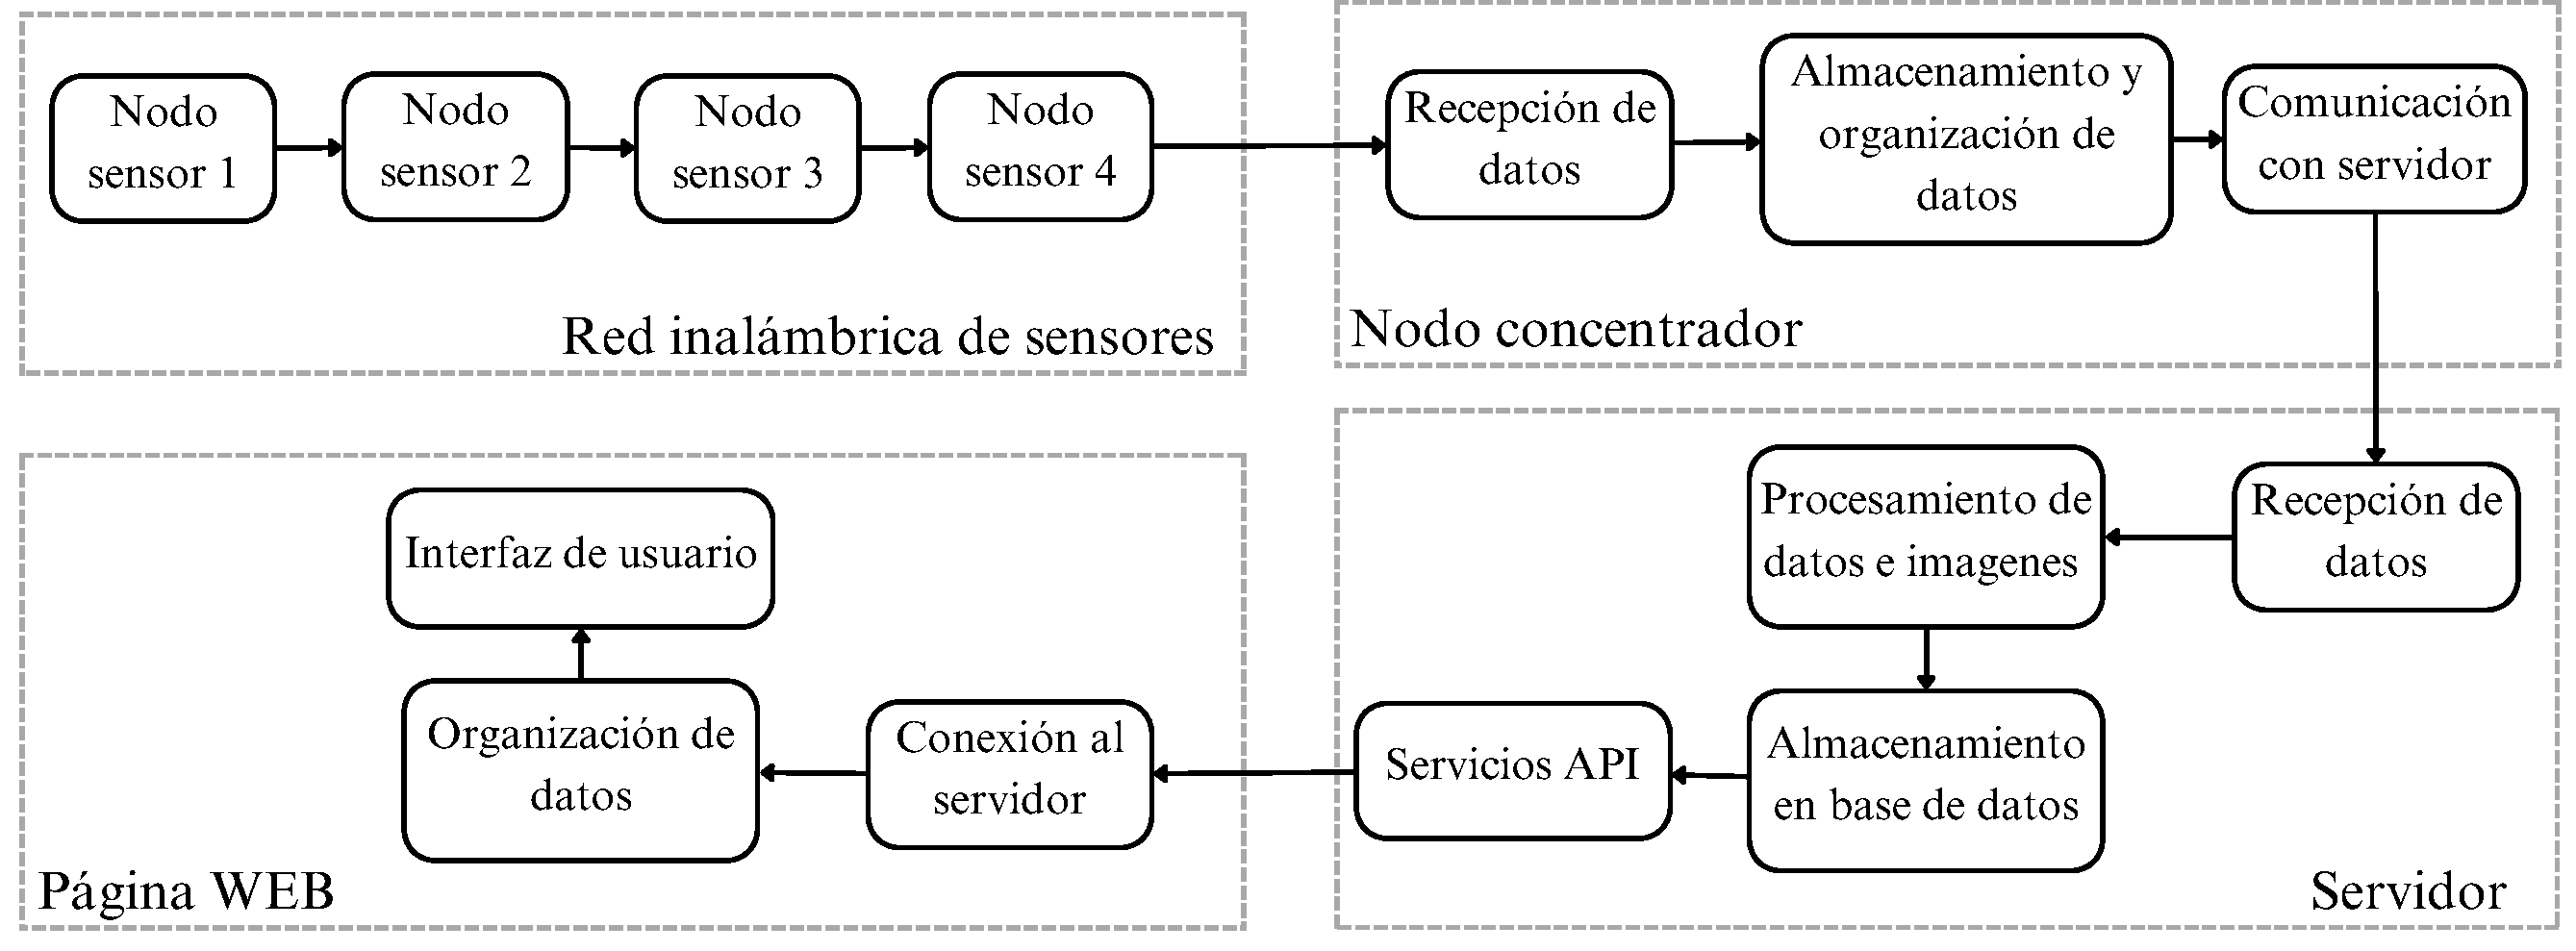
\includegraphics[width=1\textwidth]{Documento/Imagenes/Análisis/DiagramaAB2 (3).pdf}
    \caption{Diagrama a bloques del sistema.}
    \label{Dig:diagramaAB}
\end{figure}
   

\subsubsection*{Módulo 1. Red inalámbrica de sensores}

\begin{enumerate}
    \item Subsistema – Sensado de parámetros de calidad del agua \\
    \begin{figure}[H]
    \centering
    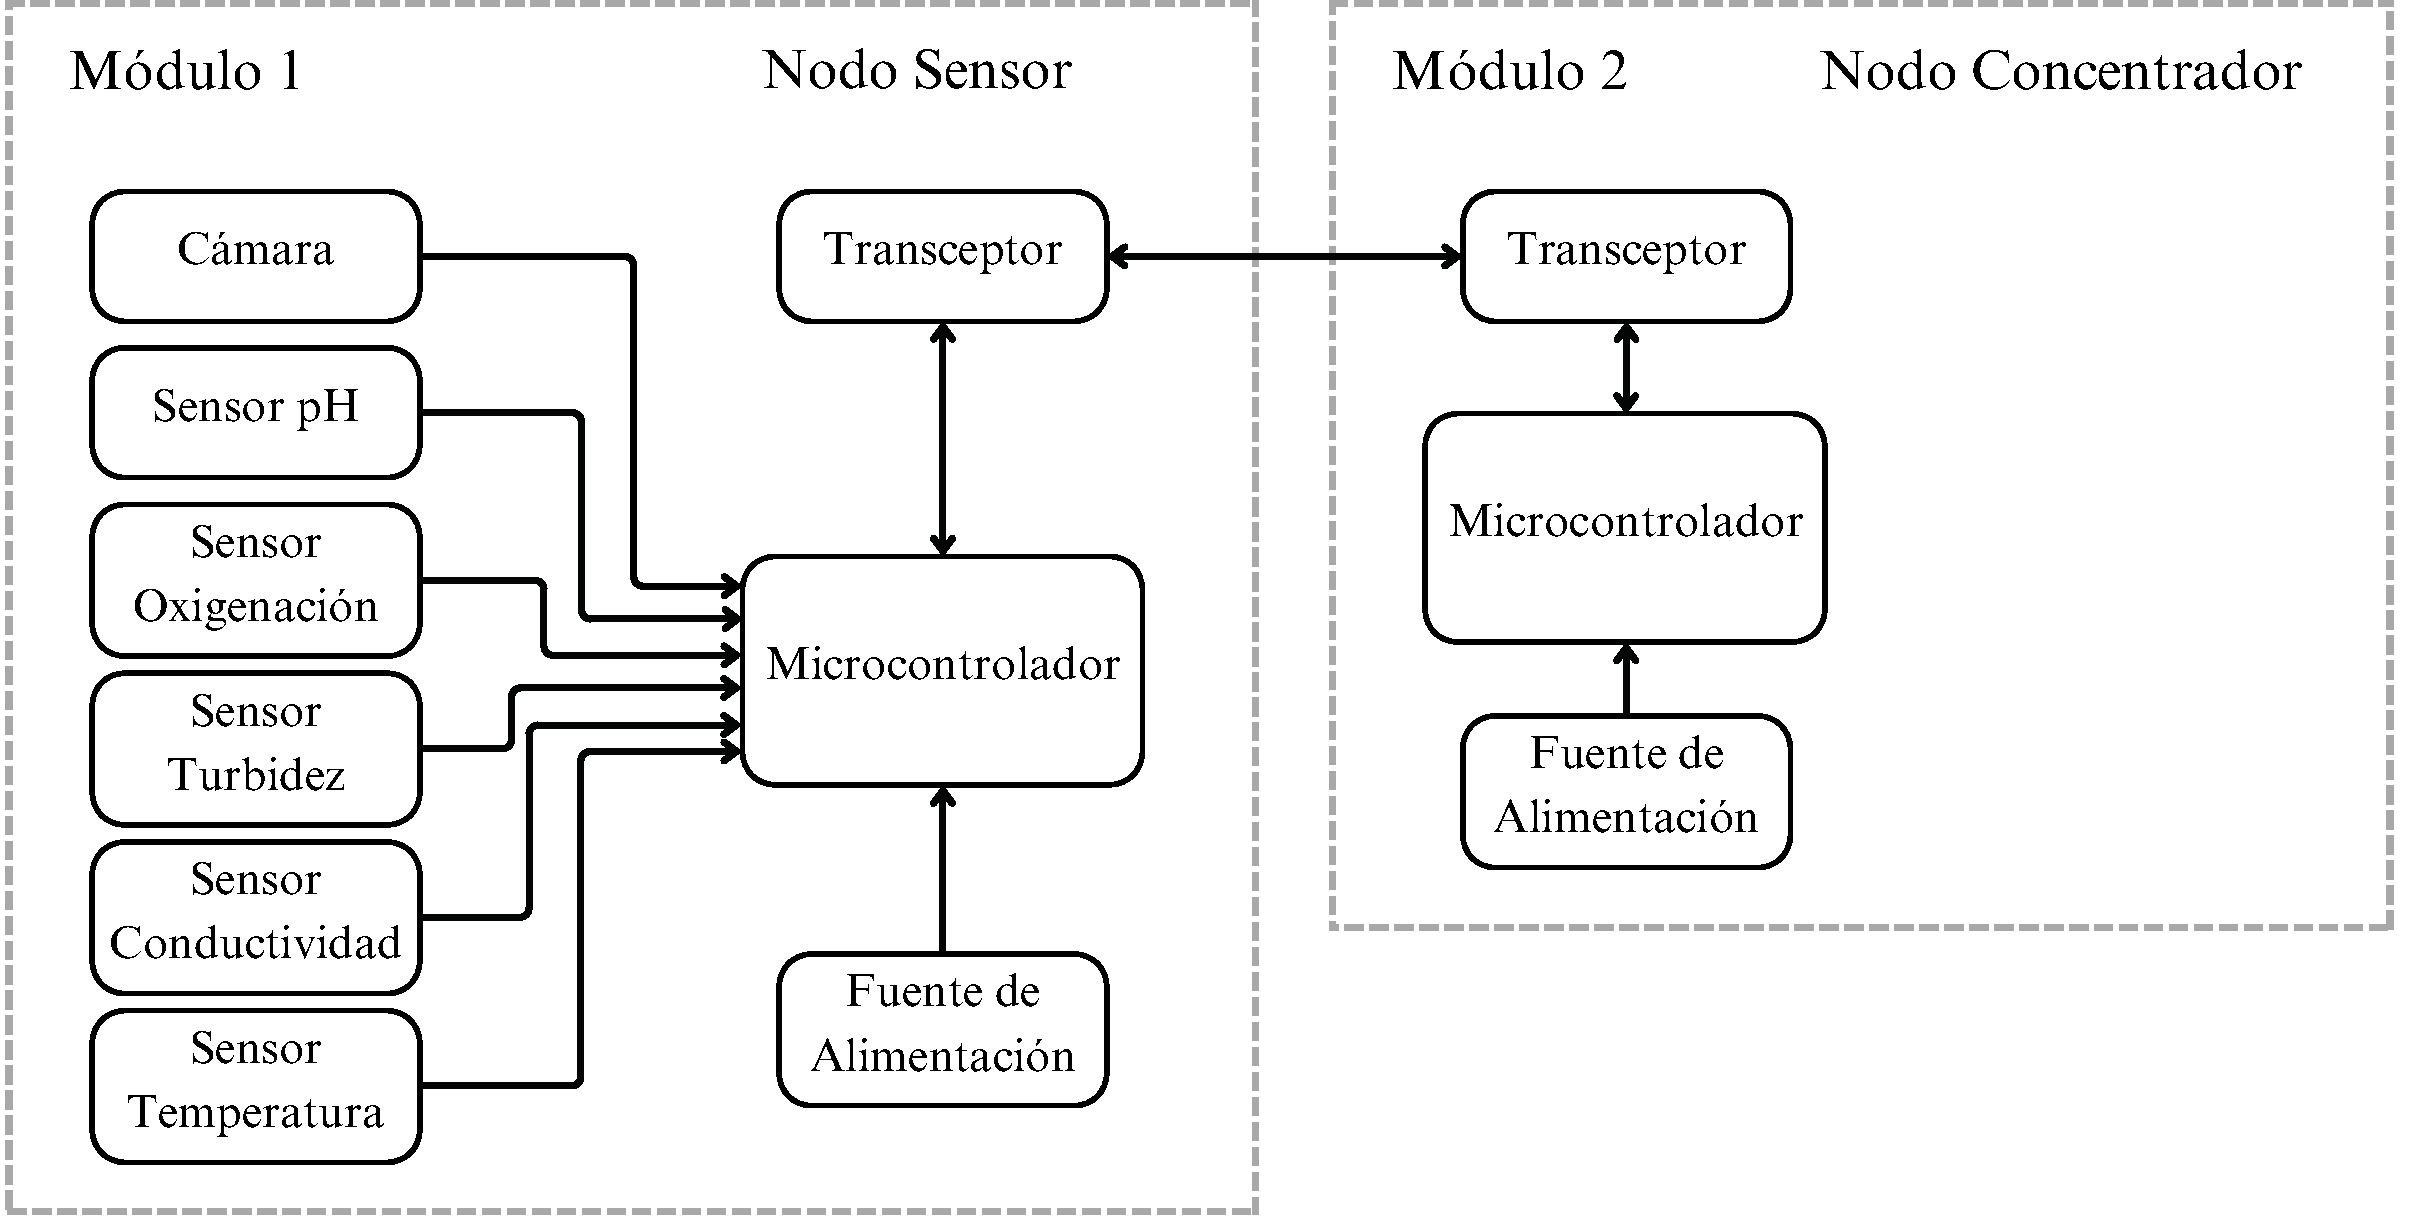
\includegraphics[width=1\textwidth]{Documento/Imagenes/Análisis/DiagramaAB2 (2).pdf}
    \caption{Diagrama a bloques del Nodeo sensor.}
    \label{Dig:diagramaAB2}
\end{figure}
    Este subsistema se encargará de obtener mediciones periódicas sobre las condiciones físico-químicas del agua mediante sensores especializados.
    \begin{itemize}
        \item Sensor de pH: permite medir el nivel de acidez del agua en intervalos definidos.
        \item Sensor de oxígeno disuelto (OD): monitorea la oxigenación del agua.
        \item Sensor de turbidez: indica la presencia de partículas suspendidas.
        \item Sensor de conductividad eléctrica: mide la concentración de iones disueltos.
        \item Sensor de temperatura: contextualiza las demás variables, ya que la temperatura afecta los valores de pH, OD y conductividad.
        \item Integración en un nodo sensor flotante: los sensores estarán integrados en un nodo con protección IP adecuada al entorno fluvial.
    \end{itemize}
    La Tabla \ref{tab:parametros_calidad_agua} presenta los rangos de medición establecidos según las recomendaciones de la Comisión Nacional del Agua (CONAGUA) \cite{conagua2022} y las Normas Oficiales Mexicanas (NOM) para análisis de agua \cite{nmx0082016, nmx0122001, nmx0382001, nmx0932000}.
    
    \begin{table}[H]
\caption{Parámetros de calidad del agua, unidades y rangos normativos}
\centering
\renewcommand{\arraystretch}{1.5}
\begin{tabular}{|p{4cm}|p{4cm}|p{4cm}|}
    \hline
    \textbf{Parámetro} & \textbf{Unidad} & \textbf{Rango normativo} \\ 
    \hline
    pH & Unidades de pH (adimensional) & 5.0 - 8.0 \\ 
    \hline
    Oxígeno disuelto (OD) & Miligramos por litro (mg/L) & $> 10$ \\ 
    \hline
    Turbidez & Unidades Nefelométricas de Turbidez (UNT) & $\leq 5$ \\ 
    \hline
    Conductividad eléctrica & Microsiemens por centímetro (\textmu S/cm) & $\leq 1,000$ \\ 
    \hline
    Temperatura & Grados Celsius (°C) & $5 - 30$ \\ 
    \hline
\end{tabular}
\label{tab:parametros_calidad_agua}
\end{table}

    \item Subsistema – Cámara \\
    Encargado de capturar imágenes periódicas de la superficie del agua para identificar residuos sólidos flotantes.
    \begin{itemize}
        \item Captura de imágenes: se utilizará una cámara compatible con el microcontrolador.
        \item Montaje en posición fija: las cámaras estarán orientadas hacia la superficie del agua.
        \item Iluminación diurna natural: se aprovechará la luz solar para evitar consumo energético adicional.
    \end{itemize}

    \item Subsistema – Microcontrolador \\
    Gestiona el funcionamiento de sensores, adquisición de datos, almacenamiento temporal y envío de información al servidor.
    \begin{itemize}
        \item Tarjeta de desarrollo: se empleará una tarjeta de bajo consumo energético y con capacidad de conectividad de largo alcance.
        \item Organización y empaquetado de datos: procesa, organiza y empaqueta los datos obtenidos de sensores y cámara antes de su transmisión.
        \item Manejo eficiente de energía: optimiza el consumo de energía en los nodos, considerando las limitaciones de alimentación en entornos remotos.
        \item Memoria: gestiona la memoria interna que almacenará temporalmente los datos antes de su transmisión.
    \end{itemize}

    \item Subsistema – Transceptor \\
    Encargado de transmitir los datos obtenidos por el nodo sensor al nodo vecino, y posteriormente al servidor central.
    \begin{itemize}
        \item Transmisión de datos: utiliza tecnologías de comunicación inalámbrica para garantizar conectividad en áreas remotas.
        \item Optimización del consumo energético: minimiza el consumo durante la transmisión mediante protocolos de bajo consumo.
        \item Enrutamiento de datos: gestiona la comunicación entre nodos mediante técnicas de reenvío.
    \end{itemize}

    \item Subsistema – Fuente de alimentación \\
    Este subsistema proporciona energía a todos los componentes del nodo.
    \begin{itemize}
        \item Batería: proporciona la energía necesaria para el funcionamiento completo del nodo.
        \item Panel solar: recarga la batería utilizando energía solar para garantizar autonomía en entornos remotos.
    \end{itemize}
\end{enumerate}

\subsubsection*{Módulo 2. Nodo concentrador}

El nodo concentrador cuenta con los mismos componentes que los nodos sensores, pero con la función adicional de recibir la información recolectada a través de la red. Este nodo centraliza los datos, los organiza y los transmite al servidor central para su procesamiento.

\begin{enumerate}
    \item Subsistema – Recepción de datos de nodos sensores
    \begin{itemize}
        \item Recepción de datos inalámbricos: debe recibir múltiples transmisiones periódicas para su almacenamiento temporal.
    \end{itemize}

    \item Subsistema – Almacenamiento temporal y organización de datos
    \begin{itemize}
        \item Almacenamiento temporal en buffer: los datos de los nodos se almacenan temporalmente en el buffer del concentrador.
        \item Organización de datos: se estructuran para facilitar su transmisión posterior.
    \end{itemize}

    \item Subsistema – Gateway
    \begin{itemize}
        \item Reenvío al servidor: envía los datos al servidor central mediante WLAN o red celular.
    \end{itemize}
\end{enumerate}

\subsubsection*{Módulo 3. Servidor}

\begin{enumerate}
    \item Subsistema – Recepción de datos del gateway
    \begin{itemize}
        \item Clasificación de datos: organiza y asigna metadatos a la información de sensores para su análisis.
    \end{itemize}

    \item Subsistema – Procesamiento de imágenes
    \begin{itemize}
        \item Detección de residuos: las imágenes son analizadas mediante visión artificial para identificar residuos flotantes.
        \item Marcas de detección: se agregan metadatos visuales a las imágenes para facilitar su interpretación.
    \end{itemize}

    \item Subsistema – Almacenamiento en base de datos
    \begin{itemize}
        \item Gestión de datos históricos: almacena la información adquirida para su análisis a largo plazo.
        \item Optimización de consultas: estructura la base de datos para recuperación rápida y eficiente.
    \end{itemize}

    \item Subsistema – API / Comunicación con página web
    \begin{itemize}
        \item API de comunicación: permite acceder a los datos e imágenes desde la página web.
        \item Enlace con la página web: proporciona una interfaz para que los usuarios consulten los resultados de monitoreo.
    \end{itemize}
\end{enumerate}

\subsubsection*{Módulo 4. Página web}

La página web permite consultar los datos recopilados por los nodos sensores y procesados en el servidor. Presenta información sobre calidad del agua y residuos flotantes en una interfaz responsiva.

\begin{enumerate}
    \item Subsistema – Conexión al servidor (API / Backend)
    \begin{itemize}
        \item API RESTful: gestiona solicitudes y respuestas de datos para visualización web.
        \item Conexión segura: implementa protocolos como HTTPS para proteger la transmisión de datos.
        \item Manejo de solicitudes y respuestas: estructura los datos enviados al frontend.
    \end{itemize}

    \item Subsistema – Interfaz de usuario (Frontend)
    \begin{itemize}
        \item HTML (estructura): define las secciones de visualización de datos.
        \item CSS (estilo): adapta el diseño para distintos dispositivos.
        \item JavaScript (interactividad): permite la actualización dinámica y navegación fluida.
    \end{itemize}
\end{enumerate}



%%%%%%%%%%%%%%%%%%%%%%%%%%%%%%%%%%%%%%%%%%%%%%%%%%%%
%          ANALISIS REQUERIMIENTOS                 %
%%%%%%%%%%%%%%%%%%%%%%%%%%%%%%%%%%%%%%%%%%%%%%%%%%%%


%%%%%%%%%%%%%%%%%%%%%%%%%%%%%%%%%%%%%%%%%%%%%%%%%%%%%
%          ANALISIS REQUERIMIENTOS                 %
%%%%%%%%%%%%%%%%%%%%%%%%%%%%%%%%%%%%%%%%%%%%%%%%%%%%


\newcounter{RF}

% Comando con contador y etiqueta opcional
\makeatletter
\newcommand{\RF}[1][]{%
  \refstepcounter{RF}%
  RF\@tempcnta=\value{RF}%
  \ifnum\@tempcnta<10 0\fi%
  \arabic{RF}%
  \if\relax#1\relax\else\label{#1}\fi%
}
\makeatother

\section{Análisis de Requerimientos}
A continuación, se presentan las tablas de los requerimientos funcionales y no funcionales identificados para el proyecto, los cuales servirán como base de referencia a lo largo de las etapas de diseño, implementación y pruebas.
\subsection{Requerimientos Funcionales}
A manera de resumen, la siguiente lista contiene los títulos de todos los requerimientos funcionales documentados a lo largo de los diferentes módulos del sistema:

\subsubsection*{Módulo 1. Red Inalámbrica de Sensores}
\begin{itemize}
    \item \textbf{RF01}: Obtención de Parámetros de Calidad del Agua.
    \item \textbf{RF02}: Protección del Nodo Sensor.
    \item \textbf{RF03}: Captura de Imágenes para Detección de Residuos.
    \item \textbf{RF04}: Coordinación del Ciclo de Operación de Sensores y Cámara
    \item \textbf{RF05}: Adquisición de Datos y Metadatos de Imagen.
    \item \textbf{RF06}: Gestión de Búfer y Memoria Temporal del Nodo Sensor.
    \item \textbf{RF07}: Estructuración y Empaquetado de Tramas de Datos.
    \item \textbf{RF08}: Garantía de Integridad de Tramas Antes de la Transmisión
    \item \textbf{RF09}: Gestión de Energía.
    \item \textbf{RF10}: Transmisión Inalámbrica de Datos.
    \item \textbf{RF11}: Proporcionar Energía a los Componentes del Nodo.
    \item \textbf{RF12}: Recarga de la Batería con Energía Solar.
\end{itemize}

\subsubsection*{Módulo 2. Nodo Concentrador}
\begin{itemize}
    \item \textbf{RF13}: Recepción de Datos de Nodos Sensores.
    \item \textbf{RF14}: Almacenamiento Temporal y Organización de Datos.
    \item \textbf{RF15}: Transmisión de Datos Organizados al Servidor Central
    \item \textbf{RF16}: Implementación de Protocolo de Detección y Corrección de Errores.
    \item \textbf{RF17}: Retransmisión de Datos en Caso de Fallo de Conexión.
\end{itemize}

\subsubsection*{Módulo 3. Servidor}
\begin{itemize}
    \item \textbf{RF18}: Recepción de Datos de Gateway.
    \item \textbf{RF19}: Organización de Datos Recibidos.
    \item \textbf{RF20}: Procesamiento de Imágenes para Cuantificación de Área de Basura.
    \item \textbf{RF21}: Almacenamiento Persistente de Datos y Metadatos.
    \item \textbf{RF22}: Exposición de Datos y Servicios Mediante API (RESTful).
\end{itemize}

\subsubsection*{Módulo 4. Página Web}
\begin{itemize}
    \item \textbf{RF23}: Consumo de Servicios del Servidor API.
    \item \textbf{RF24}: Visualización y Presentación Interactiva de Datos (Frontend).
    \item \textbf{RF25}: Permitir la Visualización de Datos Históricos.
\end{itemize}


\subsection*{Tablas de requerimientos funcionales}

%%%%%%%%%%%%%%       MODULO 1        %%%%%%%%%%%%%%%%%%%%%%%%%%%%
%%%%%%%%%%%%%%%%%%%%%%%%%%%%%%%%% subsistema sensado de parametros
\subsubsection*{Módulo 1. Red Inalámbrica de Sensores}

%%%%%%%%
% RF01
%%%%%%%%
\begin{longtable}{|l|p{12cm}|}
\hline
\textbf{\RF} & \textbf{Obtención de Parámetros de Calidad del Agua.} \\
\hline
\endfirsthead
\hline
\textbf{Versión} & 1.0 - Fecha de versión: 06/06/2025 \\
\hline
\textbf{Autor} & Equipo de Desarrollo. \\ 
\hline
\textbf{Fuente} & Documentación técnica del subsistema - Sensado de Parámetros de Calidad del Agua.\\
\hline
\textbf{Propósito} & Obtener mediciones periódicas de la calidad del agua a través de sensores especializados. \\
\hline
\textbf{Descripción} & El subsistema de sensado incluirá sensores de pH, oxígeno disuelto, turbidez, conductividad y temperatura, los cuales tomarán mediciones de los parámetros de calidad del agua en intervalos predefinidos. \\
\hline
\textbf{Especificación} & Los sensores deben medir parámetros de calidad del agua, y deben proporcionar mediciones precisas a intervalos regulares. Los datos deben ser transmitidos periódicamente al Nodo concentrador a través de una red de sensores inalámbricos para ser procesados. \\
\hline
\textbf{Prioridad} & Alta \\
\hline
\textbf{Comentarios} & La obtención de parámetros de calidad del agua es crucial para la información y prevención de problemas de contaminación en cuerpos de agua utilizados para consumo humano o en procesos industriales. El monitoreo periódico permitirá la intervención temprana. \\
\hline
\end{longtable}


%%%%%%%%
% RF02
%%%%%%%%
\begin{longtable}{|l|p{12cm}|}
\hline
\textbf{\RF} & \textbf{Protección del Nodo Sensor.} \\
\hline
\endfirsthead
\hline
\textbf{Versión} & 1.0 - Fecha de versión: 06/06/2025 \\
\hline
\textbf{Autor} & Equipo de Desarrollo \\
\hline
\textbf{Fuente} & Documentación técnica del subsistema - Sensado de Parámetros. \\
%\hline

%\textbf{Propósito} & Proteger todos los componentes en una estructura flotante que sea resistente a las condiciones acuáticas. \\
\hline
\textbf{Propósito} & Proteger los componentes del nodo sensor mediante una boya flotante con protección IP adecuada para ambientes acuáticos.  \\
\hline
\textbf{Descripción} & La boya debe estar diseñada con materiales resistentes para ser hermético al agua y debe proteger todos los componentes internos, los sensores y otros elementos electrónicos contra la humedad y el contacto con el agua. Esta estructura debe proteger los componentes internos y permitir el funcionamiento confiable cuando se utilice en cuerpos de agua. \\
\hline
\textbf{Especificación} & La estructura del nodo sensor debe tener una protección mínima de IP68, lo que asegura que es impermeable al agua y polvo. Además, el nodo debe ser capaz de soportar el movimiento brusco en condiciones desfavorables para el sistema, sin comprometer su funcionalidad. \\
\hline
\textbf{Prioridad} & Alta \\
\hline
\textbf{Comentarios} & La protección adecuada de los sensores es esencial para asegurar su rendimiento y vida útil en ambientes acuáticos. \\
\hline
\end{longtable}

%%%%%%%%
% RF03
%%%%%%%%
%%%%%%%%%%%%%%%%%%%%%%%%%%%%%%%%%% subsistema camara
\begin{longtable}{|l|p{12cm}|}
\hline
\textbf{\RF} & \textbf{Captura de Imágenes para Detección de Residuos.} \\
\hline
\endfirsthead
\hline
\textbf{Versión} & 1.0 - Fecha de versión: 06/06/2025 \\
\hline
\textbf{Autor} & Equipo de Desarrollo \\
\hline
\textbf{Fuente} & Documentación técnica del subsistema - Camára. \\
\hline
\textbf{Propósito} & Capturar imágenes periódicas de la superficie del agua para permitir la cuantificación del área cubierta por cúmulos de residuos flotantes. \\
\hline
\textbf{Descripción} & El sistema debe utilizar una cámara de bajo consumo energético para capturar imágenes de la superficie del agua, las cuales serán transmitidas al Servidor para su procesamiento. El nodo sensor solo gestionará una imagen a la vez en su memoria antes de su transmisión. \\
\hline
\textbf{Especificación} & La imagen original debe ser almacenada temporalmente y transmitida al nodo concentrador para su posterior envío al servidor central sin procesamiento ni clasificación previo en el nodo sensor. El nodo sensor no debe almacenar más de una imagen de 640×640 simultáneamente para su procesamiento y transmisión. \\
\hline
\textbf{Prioridad} & Alta \\
\hline
\textbf{Comentarios} & La captura precisa de imágenes es esencial para identificar residuos flotantes en la superficie del agua. La cámara debe ser capaz de operar en condiciones de luz natural y estar protegida de las condiciones ambientales adversas. \\
\hline
\end{longtable}

%%%%%%%%
% RF04
%%%%%%%%
%%%%%%%%%%%%%%%%%%%%%%%%%%%%%%%%%%% subsistema-Microcontrolador
\begin{longtable}{|l|p{12cm}|}
\hline
\textbf{\RF[rf:coordinacion_sensores]} & \textbf{Coordinación del Ciclo de Operación de Sensores y Cámara} \\
\hline
\endfirsthead
\hline
\textbf{Versión} & 1.0 - Fecha de versión: 06/06/2025 \\
\hline
\textbf{Autor} & Equipo de Desarrollo \\
\hline
\textbf{Fuente} & Documentación técnica del subsistema - Microcontrolador. \\
\hline
\textbf{Propósito} & Coordinar y sincronizar la activación y desactivación de los componentes, optimizando el consumo energético, para asegurar la adquisición de datos de manera eficiente. \\
\hline
\textbf{Descripción} & El microcontrolador deberá gestionar un ciclo de operación predefinido que activará secuencialmente los sensores y la cámara solo cuando sea necesario, y los pondrá en modo de reposo. \\
\hline
\textbf{Especificación} &  El microcontrolador deberá ser capaz de activar y desactivar los componentes eficientemente. El sistema debe asegurar que los componentes no esenciales entren en modo de reposo o baja energía cuando el ciclo de adquisición no esté activo. \\
\hline
\textbf{Prioridad} & Alta \\
\hline
\textbf{Comentarios} & La coordinación eficiente es esencial para garantizar que los datos y las imágenes se adquieran sin interferencias ni retrasos y que la autonomía del sistema se mantenga. \\
\hline
\end{longtable}

%%%%%%%%
% RF05
%%%%%%%%
%%%%%%%%%%%%%%%%%%%%%%%%%%%%%%%%%%% subsistema-Microcontrolador
\begin{longtable}{|l|p{12cm}|}
\hline
\textbf{\RF} & \textbf{Adquisición de Datos y Metadatos de Imagen.} \\
\hline
\endfirsthead
\hline
\textbf{Versión} & 1.0 - Fecha de versión: 06/06/2025 \\
\hline
\textbf{Autor} & Equipo de Desarrollo \\
\hline
\textbf{Fuente} & Documentación técnica del subsistema - Microcontrolador. \\
\hline
\textbf{Propósito} & Obtener las mediciones de los sensores y la captura de la imagen, asegurando su entrega al búfer para su posterior empaquetado y transmisión. \\
\hline
\textbf{Descripción} & Una vez activados, los sensores y la cámara deberán entregar sus datos y capturas, los cuales serán almacenados en el búfer del microcontrolador. \\
\hline
\textbf{Especificación} &  El sistema deberá adquirir mediciones de pH, turbidez, oxígeno disuelto, conductividad y temperatura conforme al ciclo de operación coordinado y almacenar los datos de los sensores y las imágenes temporalmente en el búfer del nodo sensor hasta su transmisión al nodo concentrador. \\
\hline
\textbf{Prioridad} & Alta \\
\hline
\textbf{Comentarios} & La correcta adquisición y almacenamiento temporal son pasos críticos para garantizar la integridad y disponibilidad de toda la información (parámetros e imágenes) antes de que se empaqueten y se envíen al servidor. \\
\hline
\end{longtable}

%%%%%%%%
% RF06
%%%%%%%%
\begin{longtable}{|l|p{12cm}|}
\hline
\textbf{\RF} & \textbf{Gestión de Búfer y Memoria Temporal del Nodo Sensor.} \\
\hline
\endfirsthead
\hline
\textbf{Versión} & 1.0 - Fecha de versión: 06/06/2025 \\
\hline
\textbf{Autor} & Equipo de Desarrollo \\
\hline
\textbf{Fuente} & Documentación técnica del subsistema - Microcontrolador. \\
\hline
\textbf{Propósito} & Gestionar la memoria interna del microcontrolador para almacenar temporalmente los datos adquiridos (sensores y la imagen única) antes de su transmisión, evitando la sobrecarga y asegurando la no pérdida de datos. \\
\hline
\textbf{Descripción} & 	El microcontrolador debe utilizar su memoria interna para almacenar de forma temporal los datos adquiridos de los sensores y una única imagen antes de que sean transmitidos al nodo concentrador. La memoria debe gestionarse eficientemente para evitar la sobrecarga. \\
\hline
\textbf{Especificación} & El microcontrolador debe ser capaz de almacenar los datos de todos los sensores y una sola imagen de 640×640 antes de la transmisión. El sistema debe permitir el borrado o sobrescritura de datos antiguos cuando la memoria esté llena, para garantizar la disponibilidad de espacio para nuevas mediciones. \\
\hline
\textbf{Prioridad} & Alta \\
\hline
\textbf{Comentarios} & 	La gestión de memoria es crucial para asegurar que los datos no se pierdan antes de ser transmitidos, lo que podría comprometer el análisis posterior. \\
\hline
\end{longtable}


%%%%%%%%
% RF07
%%%%%%%%

\begin{longtable}{|l|p{12cm}|}
\hline
\textbf{\RF[rf:Empaquetado_datos]} & \textbf{Estructuración y Empaquetado de Tramas de Datos.} \\
\hline
\endfirsthead
\hline
\textbf{Versión} & 1.0 - Fecha de versión: 06/06/2025 \\
\hline
\textbf{Autor} & Equipo de Desarrollo \\
\hline
\textbf{Fuente} & Documentación técnica del subsistema - Microcontrolador. \\
\hline
\textbf{Propósito} & Organizar y empaquetar los datos obtenidos de los sensores y cámara en tramas de información de manera estructurada para su eficiente transmisión y posterior procesamiento. \\
\hline
\textbf{Descripción} & El microcontrolador debe organizar los datos adquiridos de los sensores y cámara en tramas de información, incluyendo campos como tipo de medición, valor, fecha y hora. \\
\hline
\textbf{Especificación} & Las tramas deben estar estructuradas de manera que contengan campos definidos como: tipo de medición, valor de la medición, fecha y hora de la medición, y cualquier metadato necesario. \\
\hline
\textbf{Prioridad} & Alta \\
\hline
\textbf{Comentarios} & El correcto empaquetado de las tramas de información es esencial para garantizar la fiabilidad de los datos. La estructura de las tramas debe ser clara y uniforme. \\
\hline
\end{longtable}

%%%%%%%%
% RF08
%%%%%%%%
\begin{longtable}{|l|p{12cm}|}
\hline
\textbf{\RF} & \textbf{Garantía de Integridad de Tramas Antes de la Transmisión} \\
\hline
\endfirsthead
\hline
\textbf{Versión} & 1.0 - Fecha de versión: 06/06/2025 \\
\hline
\textbf{Autor} & Equipo de Desarrollo \\
\hline
\textbf{Fuente} & Documentación técnica del subsistema - Microcontrolador. \\
\hline
\textbf{Propósito} & Asegurar que las tramas de información empaquetadas estén completas, sin errores, y listas para su transmisión al nodo concentrador. \\
\hline
\textbf{Descripción} & Una vez empaquetados (RF0\ref{rf:Empaquetado_datos}), el microcontrolador debe aplicar métodos de verificación (ej. checksum) para asegurar que las tramas de datos están completas y sin datos faltantes o errores internos antes de iniciar la transmisión. \\
\hline
\textbf{Especificación} & El sistema debe asegurar que las tramas sean completas, sin datos faltantes, y sin errores de transmisión , y estas tramas deben ser enviadas al servidor o nodo concentrador de manera periódica, en intervalos predefinidos, asegurando que todos los datos sean correctamente transmitidos y almacenados para su análisis posterior. \\
\hline
\textbf{Prioridad} & Alta \\
\hline
\textbf{Comentarios} & Esta validación previa es un paso crítico para reducir la tasa de error en la transmisión inalámbrica y garantizar la calidad de los datos. \\
\hline
\end{longtable}



%%%%%%%%
% RF09
%%%%%%%%
\begin{longtable}{|l|p{12cm}|}
\hline
\textbf{\RF} & \textbf{Gestión de Energía.} \\
\hline
\endfirsthead
\hline
\textbf{Versión} & 1.0 - Fecha de versión: 06/06/2025 \\
\hline
\textbf{Autor} & Equipo de Desarrollo \\
\hline
\textbf{Fuente} & Documentación técnica del subsistema - Microcontrolador. \\
\hline
\textbf{Propósito} & Optimizar el consumo energético de los sensores y otros componentes del sistema para garantizar su funcionamiento eficiente en entornos remotos. \\
\hline
\textbf{Descripción} & El microcontrolador debe gestionar el consumo energético de los sensores y otros componentes, asegurando que solo estén activos cuando sea necesario y que los componentes entren en modo de reposo para maximizar la duración de la batería. \\
\hline
\textbf{Especificación} & El microcontrolador debe ser capaz de activar y desactivar los sensores y otros componentes del sistema de forma eficiente, gestionando el consumo de energía para operar durante largos períodos sin recargar. \\
\hline
\textbf{Prioridad} & Alta \\
\hline
\end{longtable}

%%%%%%%%
% RF10
%%%%%%%%
%%%%%%%%%%%%%%%%%%%%%%%%%% subsistema transceptor
\begin{longtable}{|l|p{12cm}|}
\hline
\textbf{\RF} & \textbf{Transmisión Inalámbrica de Datos.} \\
\hline
\endfirsthead
\hline
\textbf{Versión} & 1.0 - Fecha de versión: 06/06/2025 \\
\hline
\textbf{Autor} & Equipo de Desarrollo \\
\hline
\textbf{Fuente} & Documentación técnica del subsistema - Transceptor. \\
\hline
\textbf{Propósito} & Asegurar que los datos obtenidos por el nodo sensor sean transmitidos de manera inalámbrica al nodo vecinos para su procesamiento y análisis. \\
\hline
\textbf{Descripción} & Los nodos sensores deben transmitir los datos adquiridos a través de tecnologías inalámbricas, al nodo vecino, posteriormente al nodo concentrador. La transmisión debe ser confiable y asegurar que no haya pérdida de información. \\
\hline
\textbf{Especificación} & Los datos deben ser transmitidos en paquetes de datos estructurados al nodo concentrador. El sistema debe operar eficientemente en distancias de al menos 50 metros entre nodos y sin pérdida de datos. Se deben utilizar tecnologías de comunicación inalámbrica confiables para mantener la calidad de la transmisión. \\
\hline
\textbf{Prioridad} & Alta \\
\hline
\textbf{Comentarios} & La transmisión inalámbrica proporciona flexibilidad y reduce los costos de instalación, ya que no requiere cableado físico. Es esencial garantizar que los datos se transmitan sin pérdidas y que la red sea resistente a interferencias para asegurar la continuidad del monitoreo. \\
\hline
\end{longtable}


%%%%%%%%
% RF11
%%%%%%%%
%%%%%%%%%%%%%%%% subsistema fuente de alimentacion 

\begin{longtable}{|l|p{12cm}|}
\hline
\textbf{\RF} & \textbf{Proporcionar Energía a los Componentes del Nodo.} \\
\hline
\endfirsthead
\hline
\textbf{Versión} & 1.0 - Fecha de versión: 06/06/2025 \\
\hline
\textbf{Autor} & Equipo de Desarrollo \\
\hline
\textbf{Fuente} & Documentación técnica del subsistema - Fuente de Alimentación. \\
\hline
\textbf{Propósito} & Asegurar que todos los componentes del nodo, incluidos el microcontrolador, los sensores, la cámara y el transceptor, reciban la energía necesaria para su funcionamiento. \\
\hline
\textbf{Descripción} & El subsistema debe ser capaz de proporcionar energía de manera continua a todos los componentes del nodo, de modo que el sistema funcione de forma autónoma sin depender de fuentes externas de energía. \\
\hline
\textbf{Especificación} & La batería debe proporcionar energía suficiente para el funcionamiento de los componentes del nodo durante un período mínimo de 24 horas sin necesidad de recarga. La batería debe ser lo suficientemente potente para soportar el consumo combinado de todos los dispositivos conectados en el nodo. \\
\hline
\textbf{Prioridad} & Alta \\
\hline
\textbf{Comentarios} & Este subsistema es fundamental para que el sistema funcione de manera autónoma en entornos remotos donde el acceso a fuentes de energía externas es limitado o inexistente. \\
\hline
\end{longtable}


%%%%%%%%
% RF12
%%%%%%%%
\begin{longtable}{|l|p{12cm}|}
\hline
\textbf{\RF} & \textbf{Recarga de la Batería con Energía Solar.} \\
\hline
\endfirsthead
\hline
\textbf{Versión} & 1.0 - Fecha de versión: 06/06/2025 \\
\hline
\textbf{Autor} & Equipo de Desarrollo \\
\hline
\textbf{Fuente} & Documentación técnica del subsistema de Fuente de Alimentación. \\
\hline
\textbf{Propósito} & Asegurar que la batería se recargue utilizando energía solar de manera continua para mantener el funcionamiento autónomo del nodo. \\
\hline
\textbf{Descripción} & El panel solar debe ser capaz de recargar la batería durante el día, aprovechando la energía solar, para que el nodo siga funcionando de manera autónoma. \\
\hline
\textbf{Especificación} & El panel solar debe recargar completamente la batería durante aproximadamente 6 horas de luz solar directa. El sistema debe tener circuitos de protección para evitar sobrecarga o daño a la batería. \\
\hline
\textbf{Prioridad} & Alta \\
\hline
\textbf{Comentarios} & Este subsistema es esencial para garantizar el funcionamiento continuo del sistema en entornos remotos y ayuda a reducir la dependencia de fuentes externas de energía. \\
\hline
\end{longtable}


%%%%%%%%%%%%%%%%%%           MODULO 2        %%%%%%%%%%%%%%%%%%%%%%%

\subsubsection*{Módulo 2. Nodo Concentrador}

%%%%%%%%
% RF13
%%%%%%%%
\begin{longtable}{|l|p{12cm}|}
\hline
\textbf{\RF} & \textbf{Recepción de Datos de Nodos Sensores.} \\
\hline
\endfirsthead
\hline
\textbf{Versión} & 1.0 - Fecha de versión: 06/06/2025 \\
\hline
\textbf{Autor} & Equipo de Desarrollo \\
\hline
\textbf{Fuente} & Documentación técnica del subsistema - Recepción de datos de nodos sensores. \\
\hline
\textbf{Propósito} & Asegurar que el nodo concentrador pueda recibir datos de los nodos sensores de manera confiable y periódica. \\
\hline
\textbf{Descripción} & El subsistema debe ser capaz de recibir los datos transmitidos desde el último nodo sensor a través de la red inalámbrica. \\
\hline
\textbf{Especificación} & El nodo concentrador debe ser capaz de recibir múltiples transmisiones de datos periódicas del nodo sensor anterior a él sin perder información. Los datos deben ser recibidos en un formato estructurado y organizado para su almacenamiento temporal. \\
\hline
\textbf{Prioridad} & Alta \\
\hline
\textbf{Comentarios} & La confiabilidad en la recepción de los datos es esencial para evitar pérdidas de información y garantizar que todos los parámetros monitoreados sean procesados correctamente. \\
\hline
\end{longtable}

%%%%%%%%
% RF14
%%%%%%%%
\begin{longtable}{|l|p{12cm}|}
\hline
\textbf{\RF} & \textbf{Almacenamiento Temporal y Organización de Datos.} \\
\hline
\endfirsthead
\hline
\textbf{Versión} & 1.0 - Fecha de versión: 06/06/2025 \\
\hline
\textbf{Autor} & Equipo de Desarrollo \\
\hline
\textbf{Fuente} & Documentación técnica del subsistema - Almacenamiento Temporal y Organización de Datos. \\
\hline
\textbf{Propósito} & Almacenar temporalmente los datos recibidos de los nodos sensores en el buffer del nodo concentrador y organizarlos para su posterior transmisión al servidor central. \\
\hline
\textbf{Descripción} & El subsistema debe ser capaz de recibir los datos de los nodos sensores transmitidos por el nodo anterior y almacenarlos de manera temporal en el buffer del nodo concentrador. Además, debe organizar los datos de forma estructurada, asegurando que sean fácilmente accesibles y listos para ser transmitidos al servidor central. \\
\hline
\textbf{Especificación} & Los datos recibidos deben ser almacenados temporalmente en el buffer del nodo concentrador, y deben ser organizados en una estructura que facilite su acceso y transmisión posterior. \\
\hline
\textbf{Prioridad} & Alta \\
\hline
\textbf{Comentarios} & El almacenamiento temporal y la organización eficiente de los datos son esenciales para asegurar que la información se mantenga accesible y lista para su transmisión rápida al servidor sin pérdida de datos. \\
\hline
\end{longtable}

%%%%%%%%
% RF15
%%%%%%%%
\begin{longtable}{|l|p{12cm}|}
\hline
\textbf{\RF} & \textbf{Transmisión de Datos Organizados al Servidor Central} \\
\hline
\endfirsthead
\hline
\textbf{Versión} & 1.0 - Fecha de versión: 06/06/2025 \\
\hline
\textbf{Autor} & Equipo de Desarrollo \\
\hline
\textbf{Fuente} & Documentación técnica del subsistema - Gateway. \\
\hline
\textbf{Propósito} & Enviar los datos procesados y organizados al servidor central para su almacenamiento y análisis. \\
\hline
\textbf{Descripción} & El nodo concentrador debe transmitir los datos organizados y procesados al servidor central utilizando una red confiable (WLAN o enlace celular). La transmisión debe ser eficiente y sin pérdidas de datos. \\
\hline
\textbf{Especificación} & El nodo concentrador debe enviar los datos al servidor central utilizando una conexión estable y confiable , y si es necesario, se deben utilizar enlaces celulares para garantizar la conectividad remota , y el sistema debe garantizar que la transmisión sea segura y sin errores con algún método de conexión de errores. \\
\hline
\textbf{Prioridad} & Alta \\
\hline
\textbf{Comentarios} & La transmisión de los datos al servidor es esencial para el procesamiento y almacenamiento a largo plazo. Debe asegurarse que la red utilizada sea confiable y no haya pérdidas de datos durante el envío. \\
\hline
\end{longtable}

%%%%%%%%
% RF16
%%%%%%%%
\begin{longtable}{|l|p{12cm}|}
\hline
\textbf{\RF} & \textbf{Implementación de Protocolo de Detección y Corrección de Errores.} \\
\hline
\endfirsthead
\hline
\textbf{Versión} & 1.0 - Fecha de versión: 06/06/2025 \\
\hline
\textbf{Autor} & Equipo de Desarrollo \\
\hline
\textbf{Fuente} & Documentación técnica del subsistema - Gateway. \\
\hline
\textbf{Propósito} &  Asegurar que la transmisión de datos al servidor central sea segura y sin errores mediante la aplicación de un método de corrección de errores. \\
\hline
\textbf{Descripción} & El nodo concentrador debe implementar un mecanismo o protocolo (ej. control de flujo, CRC) que permita la detección y corrección de errores durante la transmisión al servidor central, garantizando la integridad de los datos. \\
\hline
\textbf{Especificación} & El sistema debe garantizar que la transmisión sea segura y sin errores con algún método de conexión de errores, y deberá realizar una validación de la trama recibida por el servidor (ACK/NACK) para confirmar la entrega exitosa de los datos. \\
\hline
\textbf{Prioridad} & Alta \\
\hline
\textbf{Comentarios} & Este requerimiento es la base técnica que soporta el requisito funcional de retransmisión en caso de fallo, mejorando la fiabilidad general del sistema. \\
\hline
\end{longtable}

%%%%%%%%
% RF17
%%%%%%%%
\begin{longtable}{|l|p{12cm}|}
\hline
\textbf{\RF} & \textbf{Retransmisión de Datos en Caso de Fallo de Conexión.} \\
\hline
\endfirsthead
\hline
\textbf{Versión} & 1.0 - Fecha de versión: 06/06/2025 \\
\hline
\textbf{Autor} & Equipo de Desarrollo \\
\hline
\textbf{Fuente} & Documentación técnica del subsistema - Gateway. \\
\hline
\textbf{Propósito} & Asegurar que los datos se retransmitan en caso de fallo de conexión hasta lograr su entrega exitosa al servidor. \\
\hline
\textbf{Descripción} & El sistema debe ser capaz de retransmitir los datos cada vez que se detecte un fallo de conexión con el servidor, hasta que la transmisión se realice con éxito. \\
\hline
\textbf{Especificación} & El sistema debe realizar retransmisiones automáticas de los datos en intervalos predefinidos si no recibe confirmación de entrega exitosa. La retransmisión debe continuar hasta que el servidor confirme la recepción exitosa de los datos. \\
\hline
\textbf{Prioridad} & Alta \\
\hline
\textbf{Comentarios} & La retransmisión de datos es crítica para asegurar que los datos no se pierdan en caso de fallos de comunicación, garantizando la integridad de la información. \\
\hline
\end{longtable}



%%%%%%%%%%%%%%%     MODULO 3. SERVIDOR
\subsubsection*{Módulo 3. Servidor}

%   subsistema 1
%%%%%%%%
% RF18
%%%%%%%%
\begin{longtable}{|l|p{12cm}|}
\hline
\textbf{\RF} & \textbf{Recepción de Datos de Gateway.} \\
\hline
\endfirsthead
\hline
\textbf{Versión} & 1.0 - Fecha de versión: 06/06/2025 \\
\hline
\textbf{Autor} & Equipo de Desarrollo \\
\hline
\textbf{Fuente} & Documentación técnica del subsistema - Recepción de datos de gateway. \\
\hline
\textbf{Propósito} & Recibir los datos enviados por el gateway para su posterior organización y almacenamiento. \\
\hline
\textbf{Descripción} & El servidor debe ser capaz de recibir los datos transmitidos por el gateway desde los nodos sensores. \\
\hline
\textbf{Especificación} & El servidor debe ser capaz de recibir múltiples transmisiones de datos de manera periódica. Los datos deben ser almacenados en una base de datos estructurada para su posterior análisis. \\
\hline
\textbf{Prioridad} & Alta \\
\hline
\textbf{Comentarios} & La recepción de datos confiable es esencial para evitar pérdidas de información que puedan afectar el análisis posterior. \\
\hline
\end{longtable}

%%%%%%%%
% RF19
%%%%%%%%
\begin{longtable}{|l|p{12cm}|}
\hline
\textbf{\RF} & \textbf{Organización de Datos Recibidos.} \\
\hline
\endfirsthead
\hline
\textbf{Versión} & 1.0 - Fecha de versión: 06/06/2025 \\
\hline
\textbf{Autor} & Equipo de Desarrollo \\
\hline
\textbf{Fuente} & Documentación técnica del subsistema - Recepción de  datos de Gateway. \\
\hline
\textbf{Propósito} & Organizar los datos recibidos para su almacenamiento y análisis eficiente. \\
\hline
\textbf{Descripción} & El servidor debe organizar los datos procesados de manera estructurada, clasificando los datos por tipo de medición, fecha, hora y otros metadatos. \\
\hline
\textbf{Especificación} & Los datos deben ser organizados en una base de datos estructurada que permita consultas rápidas y eficientes. \\
\hline
\textbf{Prioridad} & Alta \\
\hline
\textbf{Comentarios} & La organización eficiente de los datos permite un acceso rápido y preciso para análisis futuros y toma de decisiones. \\
\hline
\end{longtable}
 
%   subsistema 2 proceso de imagenes
%%%%%%%%
% RF20
%%%%%%%%
\begin{longtable}{|l|p{12cm}|}
\hline
\textbf{\RF} & \textbf{Procesamiento de Imágenes para Cuantificación de Área de Basura.} \\
\hline
\endfirsthead
\hline
\textbf{Versión} & 1.0 - Fecha de versión: 06/06/2025 \\
\hline
\textbf{Autor} & Equipo de Desarrollo \\
\hline
\textbf{Fuente} & Documentación técnica del subsistema - Procesamiento de Imágenes. \\
\hline
\textbf{Propósito} & Procesar las imágenes enviadas por el nodo concentrador, aplicar algoritmos de visión artificial y generar un valor numérico que represente el área cubierta por los cúmulos de residuos flotantes. \\
\hline
\textbf{Descripción} & El sistema debe procesar las imágenes enviadas desde el nodo concentrador, aplicar algoritmos de visión artificial para detectar cúmulos de residuos sólidos flotantes, y calcular el área que cubren en la superficie del agua. El resultado debe ser un metadato numérico que se adjuntará a la imagen procesada. \\
\hline
\textbf{Especificación} & El sistema debe ser capaz de procesar imágenes, aplicar algoritmos de visión artificial (ej. YOLOv8 o segmentación) para detectar los cúmulos de residuos flotantes y generar un metadato numérico del área cubierta para su análisis y posterior almacenamiento. \\
\hline
\textbf{Prioridad} & Alta \\
\hline
\textbf{Comentarios} & La captura precisa de imágenes es esencial para la posterior cuantificación del área de residuos flotantes en el servidor. El uso de la imagen original de 640×640 requiere una alta eficiencia de compresión en el nodo sensor para mitigar el riesgo de sobrecarga de la red inalámbrica de baja potencia. \\
\hline
\end{longtable}

%%%%%%%%
% RF21
%%%%%%%%
%   subsistema 3. Almacenamiento en base de datos
\begin{longtable}{|l|p{12cm}|}
\hline
\textbf{\RF} & \textbf{Almacenamiento Persistente de Datos y Metadatos.} \\
\hline
\endfirsthead
\hline
\textbf{Versión} & 1.0 - Fecha de versión: 06/06/2025 \\
\hline
\textbf{Autor} & Equipo de Desarrollo \\
\hline
\textbf{Fuente} & Documentación técnica del subsistema - Almacenamiento en Base de Datos. \\
\hline
\textbf{Propósito} & Almacenar los datos y metadatos de los sensores y las imágenes de residuos en una base de datos para su posterior consulta. \\
\hline
\textbf{Descripción} & El servidor debe almacenar los datos procesados y organizados de los sensores y las imágenes de residuos flotantes de manera estructurada en una base de datos organizada. \\
\hline
\textbf{Especificación} & Los datos y metadatos deben ser almacenados de manera eficiente, garantizando la integridad y accesibilidad de la información histórica para su consulta. \\
\hline
\textbf{Prioridad} & Alta \\
\hline
\textbf{Comentarios} & El almacenamiento adecuado de los datos es fundamental para su acceso a largo plazo y para el análisis posterior. \\
\hline
\end{longtable}

%%%%%%%%
% RF22
%%%%%%%%
%   subsistema 4. API/Comunicación (Enlace con página web)
\begin{longtable}{|l|p{12cm}|}
\hline
\textbf{\RF} & \textbf{Exposición de Datos y Servicios Mediante API (RESTful).} \\
\hline
\endfirsthead
\hline
\textbf{Versión} & 1.0 - Fecha de versión: 06/06/2025 \\
\hline
\textbf{Autor} & Equipo de Desarrollo \\
\hline
\textbf{Fuente} & Documentación técnica del subsistema - API/Comunicación (Enlace con página web). \\
\hline
\textbf{Propósito} & Gestionar la comunicación entre el servidor y la página web, permitiendo la recuperación eficiente de los datos procesados. \\
\hline
\textbf{Descripción} & El servidor debe proporcionar una API para que la página web acceda a los datos de calidad del agua y las imágenes de residuos flotantes. \\
\hline
\textbf{Especificación} & La API RESTful debe permitir el acceso eficiente a los datos y imágenes almacenados en el servidor. La comunicación debe ser segura (utilizando HTTPS). \\
\hline
\textbf{Prioridad} & Alta \\
\hline
\textbf{Comentarios} & La integración con la página web es esencial para que los usuarios puedan consultar los datos sobre el estado del agua y los residuos flotantes. \\
\hline
\end{longtable}

%%%%%%%%%%      MODULO 3         %%%%%%%%%%%%%%%
\subsubsection*{Módulo 4. Página Web}

%%%%%%%%
% RF23
%%%%%%%%
%       subistema 1. Conexion al servidor API backend
\begin{longtable}{|l|p{12cm}|}
\hline
\textbf{\RF} & \textbf{Consumo de Servicios del Servidor API.} \\
\hline
\endfirsthead
\hline
\textbf{Versión} & 1.0 - Fecha de versión: 06/06/2025 \\
\hline
\textbf{Autor} & Equipo de Desarrollo \\
\hline
\textbf{Fuente} & Documentación técnica del subsistema - Conexión al Servidor (API/Backend). \\
\hline
\textbf{Propósito} & Gestionar la comunicación entre la página web y el servidor para la recuperación y visualización de datos. \\
\hline
\textbf{Descripción} & El subsistema debe gestionar la comunicación entre el frontend (página web) y el backend (servidor). Utilizará una API RESTful para recuperar los datos de calidad del agua y los residuos sólidos, enviando solicitudes y respondiendo con la información necesaria para la visualización en la página web. \\
\hline
\textbf{Especificación} & La API RESTful debe permitir que la página web solicite y reciba datos del servidor de forma eficiente y segura. La conexión debe ser segura (HTTPS), y el backend debe manejar las solicitudes de datos, procesarlas y responder con la información organizada y estructurada. \\
\hline
\textbf{Prioridad} & Alta \\
\hline
\textbf{Comentarios} & La seguridad en la comunicación entre la página web y el servidor es fundamental para proteger los datos y garantizar la privacidad. \\
\hline
\end{longtable}

%%%%%%%%
% RF24
%%%%%%%%
\begin{longtable}{|l|p{12cm}|}
\hline
\textbf{\RF} & \textbf{Visualización y Presentación Interactiva de Datos (Frontend).} \\
\hline
\endfirsthead
\hline
\textbf{Versión} & 1.0 - Fecha de versión: 06/06/2025 \\
\hline
\textbf{Autor} & Equipo de Desarrollo \\
\hline
\textbf{Fuente} & Documentación técnica del subsistema - Interfaz de usuario (Frontend). \\
\hline
\textbf{Propósito} & Permitir la visualización clara y atractiva de los datos de calidad del agua y residuos sólidos flotantes en la página web, incluyendo la generación de gráficos interactivos. \\
\hline
\textbf{Descripción} & La página web debe presentar los datos de forma clara, utilizando gráficos interactivos, tablas y representaciones visuales de los datos obtenidos. El diseño debe ser responsive y accesible desde diferentes dispositivos (móviles, tabletas y computadoras). \\
\hline
\textbf{Especificación} & Los gráficos deben ser actualizados dinámicamente sin necesidad de recargar la página. La visualización debe ser clara y los usuarios deben poder interactuar con los gráficos para obtener información detallada de los datos (ej. mediante tooltips o filtros). \\
\hline
\textbf{Prioridad} & Alta \\
\hline
\textbf{Comentarios} & La usabilidad es clave para garantizar que los usuarios puedan acceder a la información sin dificultades, por lo que la interactividad y la adaptabilidad de la página son esenciales. \\
\hline
\end{longtable}



%%%%%%%%
% RF25
%%%%%%%%
\begin{longtable}{|l|p{12cm}|}
\hline
\textbf{\RF} & \textbf{Permitir la Visualización de Datos Históricos.} \\
\hline
\endfirsthead
\hline
\textbf{Versión} & 1.0 - Fecha de versión: 06/06/2025 \\
\hline
\textbf{Autor} & Equipo de Desarrollo \\
\hline
\textbf{Fuente} & Documentación técnica del subsistema - Interfaz de usuario (Frontend). \\
\hline
\textbf{Propósito} & Permitir que los usuarios visualicen los datos históricos de calidad del agua y residuos sólidos flotantes. \\
\hline
\textbf{Descripción} & La página web debe permitir que los usuarios visualicen los datos históricos de los parámetros de calidad del agua y los residuos sólidos flotantes a lo largo del tiempo con la capacidad de interactuar con las fechas de monitoreo. \\
\hline
\textbf{Especificación} & Los usuarios deben poder acceder a los datos históricos mediante una interfaz que les permita ver cómo evolucionaron los parámetros de calidad del agua y los residuos flotantes. \\
\hline
\textbf{Prioridad} & Alta \\
\hline
\textbf{Comentarios} & La visualización de los datos históricos es crucial para realizar un análisis de tendencias y evaluar la evolución de la calidad del agua y la presencia de residuos. \\
\hline
\end{longtable}


%%%%%%%%%%%%%%%%%%%%%%%%%%%%%%%%%%%%%%%%%%%%%
%       Requerimientos NO FUNCIONALES       %
%%%%%%%%%%%%%%%%%%%%%%%%%%%%%%%%%%%%%%%%%%%%%
\subsection{Requerimientos No Funcionales}
Los requerimientos no funcionales definen los criterios de calidad y restricciones del sistema. A continuación, se presenta un resumen de sus títulos:

\subsubsection*{Módulo 1. Red Inalámbrica de Sensores}
\begin{itemize}
    \item \textbf{RNF01}: Precisión de los Sensores.
    \item \textbf{RNF02}: Certificación IP de la Carcasa del Nodo Sensor.
    \item \textbf{RNF03}: Calidad de la Imagen.
    \item \textbf{RNF04}: Bajo Consumo Energético del Microcontrolador.
    \item \textbf{RNF05}: Compatibilidad con Comunicaciones de Largo Alcance.
    \item \textbf{RNF06}: Gestión de Memoria para Evitar Pérdida de Datos.
    \item \textbf{RNF07}: Fiabilidad de la Comunicación Inalámbrica.
    \item \textbf{RNF08}: Consumo Energético del Transceptor.
    \item \textbf{RNF09}: Eficiencia Energética de la Fuente de Alimentación.
\end{itemize}

\subsubsection*{Módulo 2. Nodo Concentrador}
\begin{itemize}
    \item \textbf{RNF10}: Fiabilidad de la Recepción de Datos.
    \item \textbf{RNF11}: Eficiencia en el Almacenamiento Temporal.
    \item \textbf{RNF12}: Organización de Datos para Transmisión.
    \item \textbf{RNF13}: Prevención de Sobrecargas o Pérdidas por Desbordamiento de Buffer.
    \item \textbf{RNF14}: Fiabilidad en el Reenvío de Datos al Servidor.
\end{itemize}

\subsubsection*{Módulo 3. Servidor}
\begin{itemize}
    \item \textbf{RNF15}: Validación Automática de Datos Recibidos.
    \item \textbf{RNF16}: Optimización del Procesamiento y Trazabilidad del Algoritmo de Área de Basura.
    \item \textbf{RNF17}: Acceso a Datos Históricos de al Menos un Año.
    \item \textbf{RNF18}: Rendimiento y Seguridad de la API.
\end{itemize}

\subsubsection*{Módulo 4. Página Web}
\begin{itemize}
    \item \textbf{RNF19}: Accesibilidad y Responsividad de la Interfaz.
    \item \textbf{RNF20}: Diseño Claro y Estético de la Interfaz.
\end{itemize}


\subsection*{Tablas de requerimientos no funcionales}
%%%%%%%%%%      Modulo 1        %%%%%%%%%%%
%   subsistema 1. Sensado de parametros de calidad del agua

\subsubsection*{Módulo 1. Red Inalámbrica de Sensores}

%%%%%%%%
% RNF01
%%%%%%%%
\begin{longtable}{|l|p{12cm}|}
\hline
\textbf{RNF01} & \textbf{Precisión de los Sensores.} \\
\hline
\endfirsthead
\hline
\textbf{Versión} & 1.0 - Fecha de versión: 06/06/2025 \\
\hline
\textbf{Autor} & Equipo de Desarrollo \\
\hline
\textbf{Fuente} & Documentación técnica del subsistema - Sensado de Parámetros de Calida del Agua. \\
\hline
\textbf{Propósito} & Garantizar que los sensores proporcionen mediciones precisas y fiables de los parámetros de calidad del agua. \\
\hline
\textbf{Descripción} & Los sensores deben ser capaces de medir los parámetros de calidad del agua: pH, oxígeno disuelto, turbidez, conductividad, con un margen de error mínimo en la medición, cumpliendo con las normas de precisión establecidas (NOM). \\
\hline
\textbf{Especificación} & Los sensores deben cumplir con la precisión adecuada. El margen de error máximo debe ser del 2\% para turbidez y de ±0.1 unidades para el pH, y estar dentro de los límites de las Normas Oficiales Mexicanas (NOM). \\
\hline
\textbf{Prioridad} & Alta \\
\hline
\textbf{Comentarios} & La precisión de los sensores es fundamental para asegurar que los datos obtenidos sean confiables y útiles para la toma de decisiones. \\
\hline
\end{longtable}

%%%%%%%%
% RNF02
%%%%%%%%
\begin{longtable}{|l|p{12cm}|}
\hline
\textbf{RNF02} & \textbf{Certificación IP de la Carcasa del Nodo Sensor.} \\
\hline
\endfirsthead
\hline
\textbf{Versión} & 1.0 - Fecha de versión: 06/06/2025 \\
\hline
\textbf{Autor} & Equipo de Desarrollo \\
\hline
\textbf{Fuente} & Documentación técnica del subsistema - Sensado de Parámetros de Calidad del Agua. \\
\hline
\textbf{Propósito} & Garantizar que la carcasa del nodo sensor tenga una clasificación de protección IP adecuada para soportar inmersión en cuerpos de agua. \\
\hline
\textbf{Descripción} & La carcasa del nodo sensor debe contar con una clasificación IP adecuada que garantice su resistencia al agua y su capacidad para operar bajo condiciones de inmersión en cuerpos de agua, como ríos, arroyos y lagos, considerando pesos y ubicación de los componentes. \\
\hline
\textbf{Especificación} & La carcasa debe tener al menos una clasificación IP68, lo que asegura que el nodo sensor sea completamente impermeable al agua y resistente al polvo. La boya debe ser capaz de flotar sin que la funcionalidad de los componentes se vea comprometida. \\
\hline
\textbf{Prioridad} & Alta \\
\hline
\textbf{Comentarios} & La resistencia al agua es esencial para garantizar que el nodo sensor funcione correctamente en entornos acuáticos sin riesgo de fallos debido a la exposición al agua o la humedad. \\
\hline
\end{longtable}

%%%%%%%%
% RNF03
%%%%%%%%
%       subsistema 2. Camara
\begin{longtable}{|l|p{12cm}|}
\hline
\textbf{RNF03} & \textbf{Calidad de la Imagen.} \\
\hline
\endfirsthead
\hline
\textbf{Versión} & 1.0 - Fecha de versión: 06/06/2025 \\
\hline
\textbf{Autor} & Equipo de Desarrollo \\
\hline
\textbf{Fuente} & Documentación técnica del subsistema - Cámara. \\
\hline
\textbf{Propósito} & Garantizar que la cámara capture imágenes de la calidad necesaria para el cálculo preciso del área de residuos flotantes en el servidor. \\
\hline
\textbf{Descripción} & La cámara debe ser capaz de capturar imágenes nítidas y claras bajo diversas condiciones de iluminación y con la resolución 640×640 necesaria para el análisis de segmentación. \\
\hline
\textbf{Especificación} & La cámara debe ser capaz de capturar imágenes con una resolución mínima de 640×640 y una calidad de imagen que permita identificar claramente los cúmulos de residuos flotantes en el agua. La calidad de la imagen debe ser consistente incluso con variaciones de luz diurna. \\
\hline
\textbf{Prioridad} & Alta \\
\hline
\textbf{Comentarios} & La precisión en la captura de imágenes es esencial para una detección precisa de los residuos flotantes y para garantizar la calidad del análisis posterior. \\
\hline
\end{longtable}

%%%%%%%%
% RNF04
%%%%%%%%
%       subssitema 3. Microcontrolador
\begin{longtable}{|l|p{12cm}|}
\hline
\textbf{RNF04} & \textbf{Bajo Consumo Energético del Microcontrolador.} \\
\hline
\endfirsthead
\hline
\textbf{Versión} & 1.0 - Fecha de versión: 06/06/2025 \\
\hline
\textbf{Autor} & Equipo de Desarrollo \\
\hline
\textbf{Fuente} & Documentación técnica del subsistema de Microcontrolador. \\
\hline
\textbf{Propósito} & Optimizar el consumo energético del microcontrolador para maximizar la duración de la batería. \\
\hline
\textbf{Descripción} & El microcontrolador debe operar con bajo consumo energético, utilizando técnicas de bajo consumo durante períodos de inactividad (como el modo reposo). \\
\hline
\textbf{Especificación} & El microcontrolador debe consumir no más de 100 mA en su modo activo y menos de 5 mA en el modo de reposo. \\
\hline
\textbf{Prioridad} & Alta \\
\hline
\textbf{Comentarios} & El bajo consumo energético es crucial para asegurar la autonomía del sistema, especialmente en entornos remotos. \\
\hline
\end{longtable}

%%%%%%%%
% RNF05
%%%%%%%%
\begin{longtable}{|l|p{12cm}|}
\hline
\textbf{RNF05} & \textbf{Compatibilidad con Comunicaciones de Largo Alcance.} \\
\hline
\endfirsthead
\hline
\textbf{Versión} & 1.0 - Fecha de versión: 06/06/2025 \\
\hline
\textbf{Autor} & Equipo de Desarrollo \\
\hline
\textbf{Fuente} & Documentación técnica del subsistema de Microcontrolador. \\
\hline
\textbf{Propósito} & Garantizar que el microcontrolador sea compatible con tecnologías de comunicación de largo alcance. \\
\hline
\textbf{Descripción} & El microcontrolador debe ser compatible con tecnologías de comunicación de largo alcance, para garantizar la transmisión eficiente de datos entre nodos y el servidor central en áreas remotas. \\
\hline
\textbf{Especificación} & El microcontrolador debe ser compatible con LoRa o tecnologías similares como WiFI de bajo consumo y largo alcance, garantizando una transmisión de datos confiable hasta distancias de 50 m en entornos abiertos. \\
\hline
\textbf{Prioridad} & Alta \\
\hline
\textbf{Comentarios} & La compatibilidad con comunicaciones de largo alcance es clave para conectar los nodos sensores en áreas remotas sin necesidad de infraestructura de red adicional. \\
\hline
\end{longtable}

%%%%%%%%
% RNF06
%%%%%%%%
\begin{longtable}{|l|p{12cm}|}
\hline
\textbf{RNF06} & \textbf{Gestión de Memoria para Evitar Pérdida de Datos.} \\
\hline
\endfirsthead
\hline
\textbf{Versión} & 1.0 - Fecha de versión: 06/06/2025 \\
\hline
\textbf{Autor} & Equipo de Desarrollo \\
\hline
\textbf{Fuente} & Documentación técnica del subsistema de Microcontrolador. \\
\hline
\textbf{Propósito} & Garantizar que no se pierdan datos de los sensores ni la imagen única antes de ser transmitidos al servidor. \\
\hline
\textbf{Descripción} & El microcontrolador debe gestionar eficientemente la memoria para almacenar los datos temporalmente hasta su transmisión al servidor central, asegurando que no haya pérdida de información. \\
\hline
\textbf{Especificación} & La memoria interna o externa debe ser suficiente para almacenar los datos de los sensores y al menos una imagen de 640×640 antes de la transmisión. El sistema debe asegurar que esta capacidad sea suficiente para un ciclo de operación completo sin desbordamiento. \\
\hline
\textbf{Prioridad} & Alta \\
\hline
\textbf{Comentarios} & La gestión de memoria es crucial para asegurar que los datos no se pierdan antes de ser transmitidos, lo que podría comprometer el análisis posterior. \\
\hline
\end{longtable}


%%%%%%%%
% RNF07
%%%%%%%%
%       subsistema 4. Transceptor
\begin{longtable}{|l|p{12cm}|}
\hline
\textbf{RNF07} & \textbf{Fiabilidad de la Comunicación Inalámbrica.} \\
\hline
\endfirsthead
\hline
\textbf{Versión} & 1.0 - Fecha de versión: 06/06/2025 \\
\hline
\textbf{Autor} & Equipo de Desarrollo \\
\hline
\textbf{Fuente} & Documentación técnica del subsistema - Transceptor. \\
\hline
\textbf{Propósito} & Asegurar que los datos transmitidos entre los nodos sensores y el nodo concentrador lleguen de manera confiable y sin pérdidas. \\
\hline
\textbf{Descripción} & La comunicación inalámbrica entre nodos debe ser estable y confiable, garantizando que los datos transmitidos no se pierdan ni corran el riesgo de ser corrompidos. \\
\hline
\textbf{Especificación} & El sistema debe operar con una fiabilidad de transmisión mínima del 99\%, y los datos deben ser enviados sin pérdidas a través de protocolos de comunicación confiables. \\
\hline
\textbf{Prioridad} & Alta \\
\hline
\textbf{Comentarios} & La confiabilidad de la red inalámbrica es crítica, especialmente en entornos remotos, para asegurar que los datos siempre lleguen al nodo concentrador sin interrupciones. \\
\hline
\end{longtable}

%%%%%%%%
% RNF08
%%%%%%%%
\begin{longtable}{|l|p{12cm}|}
\hline
\textbf{RNF08} & \textbf{Consumo Energético del Transceptor.} \\
\hline
\endfirsthead
\hline
\textbf{Versión} & 1.0 - Fecha de versión: 06/06/2025 \\
\hline
\textbf{Autor} & Equipo de Desarrollo \\
\hline
\textbf{Fuente} & Documentación técnica del subsistema - Transceptor. \\
\hline
\textbf{Propósito} & Minimizar el consumo energético del transceptor para garantizar un funcionamiento autónomo durante períodos largos sin necesidad de recarga. \\
\hline
\textbf{Descripción} & El transceptor debe operar con un bajo consumo de energía durante el proceso de transmisión de datos, utilizando protocolos de comunicación de bajo consumo energético. \\
\hline
\textbf{Especificación} & El transceptor debe optimizar su consumo energético, limitando la transmisión de datos solo cuando sea necesario. El consumo de energía no debe exceder los 200 mA durante la transmisión de datos. \\
\hline
\textbf{Prioridad} & Alta \\
\hline
\textbf{Comentarios} & El bajo consumo energético es fundamental para maximizar la autonomía de los nodos en entornos remotos donde la energía es limitada. \\
\hline
\end{longtable}

%%%%%%%%
% RNF09
%%%%%%%%
%       subsistema 5. Fuente de Alimentacion
\begin{longtable}{|l|p{12cm}|}
\hline
\textbf{RNF09} & \textbf{Eficiencia Energética de la Fuente de Alimentación.} \\
\hline
\endfirsthead
\hline
\textbf{Versión} & 1.0 - Fecha de versión: 06/06/2025 \\
\hline
\textbf{Autor} & Equipo de Desarrollo \\
\hline
\textbf{Fuente} & Documentación técnica del subsistema - Fuente de Alimentación. \\
\hline
\textbf{Propósito} & Asegurar que la fuente de alimentación proporcione energía de manera eficiente, con la capacidad de recargar la batería utilizando energía solar. \\
\hline
\textbf{Descripción} & La fuente de alimentación debe ser capaz de proporcionar suficiente energía para todos los componentes del nodo, optimizando la duración de la batería y permitiendo su recarga utilizando energía solar. \\
\hline
\textbf{Especificación} & El panel solar debe ser capaz de recargar completamente la batería en aproximadamente 6 horas de luz solar directa, y la batería debe soportar al menos 24 horas de funcionamiento sin recarga. \\
\hline
\textbf{Prioridad} & Alta \\
\hline
\textbf{Comentarios} & El consumo eficiente de energía es crucial para garantizar el funcionamiento autónomo de los nodos en entornos remotos. La recarga solar optimiza la sostenibilidad del sistema. \\
\hline
\end{longtable}

%%%%%%%%%%%%%%%%%       Modulo 2        %%%%%%%%%%%%%%%%%%
%       subsistema 1. Recepcion de datos de nodos sensores
\subsubsection*{Módulo 2. Nodo concentrador}

%%%%%%%%
% RNF10
%%%%%%%%
\begin{longtable}{|l|p{12cm}|}
\hline
\textbf{RNF10} & \textbf{Fiabilidad de la Recepción de Datos.} \\
\hline
\endfirsthead
\hline
\textbf{Versión} & 1.0 - Fecha de versión: 06/06/2025 \\
\hline
\textbf{Autor} & Equipo de Desarrollo \\
\hline
\textbf{Fuente} & Documentación técnica del subsistema - Recepción de datos de nodos concentradores. \\
\hline
\textbf{Propósito} & Garantizar que los datos recibidos de los nodos sensores lleguen de manera confiable y sin pérdida de información. \\
\hline
\textbf{Descripción} & El subsistema debe ser capaz de recibir los datos transmitidos desde los nodos sensores de manera eficiente y sin pérdidas de información, incluso si los nodos están enviando datos de forma simultánea. \\
\hline
\textbf{Especificación} & La recepción de datos debe garantizar que no haya pérdida de paquetes ni interrupciones en la transmisión, y debe permitir la recepción de múltiples transmisiones de datos periódicas sin errores. \\
\hline
\textbf{Prioridad} & Alta \\
\hline
\textbf{Comentarios} & La fiabilidad es esencial para evitar la pérdida de datos, lo cual podría afectar el análisis y la toma de decisiones. \\
\hline
\end{longtable}

%%%%%%%%
% RNF11
%%%%%%%%
%       subsistema 2. Almacenamiento temporal y organización de datos
\begin{longtable}{|l|p{12cm}|}
\hline
\textbf{RNF11} & \textbf{Eficiencia en el Almacenamiento Temporal.} \\
\hline
\endfirsthead
\hline
\textbf{Versión} & 1.0 - Fecha de versión: 06/06/2025 \\
\hline
\textbf{Autor} & Equipo de Desarrollo \\
\hline
\textbf{Fuente} & Documentación técnica del subsistema - Almacenamiento temporal y organización de datos. \\
\hline
\textbf{Propósito} & Asegurar que los datos sean almacenados temporalmente de forma eficiente y sin sobrecargar el buffer del nodo concentrador. \\
\hline
\textbf{Descripción} & El subsistema debe ser capaz de almacenar los datos temporalmente en un buffer de manera eficiente para evitar que se pierdan o se sobrecargue el sistema. Los datos deben estar disponibles para ser procesados y enviados al servidor en el momento adecuado. \\
\hline
\textbf{Especificación} & El buffer del nodo concentrador debe tener suficiente capacidad para almacenar los datos de al menos 24 horas de monitoreo continuo. Además, el almacenamiento temporal debe tener una latencia mínima para garantizar que los datos se transmitan rápidamente al servidor una vez procesados. \\
\hline
\textbf{Prioridad} & Alta \\
\hline
\textbf{Comentarios} & La gestión eficiente del almacenamiento temporal es crucial para asegurar que no haya pérdida de datos y que el sistema opere sin interrupciones, incluso cuando los nodos sensores envíen datos de manera periódica. \\
\hline
\end{longtable}

%%%%%%%%
% RNF12
%%%%%%%%
\begin{longtable}{|l|p{12cm}|}
\hline
\textbf{RNF12} & \textbf{Organización de Datos para Transmisión.} \\
\hline
\endfirsthead
\hline
\textbf{Versión} & 1.0 - Fecha de versión: 06/06/2025 \\
\hline
\textbf{Autor} & Equipo de Desarrollo \\
\hline
\textbf{Fuente} & Documentación técnica del subsistema de Nodo Concentrador. \\
\hline
\textbf{Propósito} & Organizar los datos de forma eficiente para su transmisión posterior al servidor. \\
\hline
\textbf{Descripción} & Los datos almacenados temporalmente deben ser organizados en una estructura que permita su transmisión rápida y eficiente al servidor. La organización de los datos debe facilitar su acceso y reducir el tiempo de procesamiento. \\
\hline
\textbf{Especificación} & Los datos deben ser organizados en una estructura jerárquica o por categorías que faciliten su transmisión y procesamiento posterior, con un tiempo de acceso no mayor a 5 segundos. \\
\hline
\textbf{Prioridad} & Alta \\
\hline
\textbf{Comentarios} & Una buena organización de los datos permite reducir la latencia de transmisión y asegura que los datos se mantengan estructurados y coherentes. \\
\hline
\end{longtable}

%%%%%%%%
% RNF13
%%%%%%%%
\begin{longtable}{|l|p{12cm}|}
\hline
\textbf{RNF13} & \textbf{Prevención de Sobrecargas o Pérdidas por Desbordamiento de Buffer.} \\
\hline
\endfirsthead
\hline
\textbf{Versión} & 1.0 - Fecha de versión: 06/06/2025 \\
\hline
\textbf{Autor} & Equipo de Desarrollo \\
\hline
\textbf{Fuente} & Documentación técnica del subsistema de Gestión de Memoria. \\
\hline
\textbf{Propósito} & Evitar la sobrecarga o pérdida de datos debido a desbordamientos de buffer en el sistema. \\
\hline
\textbf{Descripción} & El sistema debe estar diseñado para prevenir sobrecargas y desbordamientos de buffer en cualquier etapa del proceso de almacenamiento temporal de datos, garantizando que no haya pérdidas de información debido a la incapacidad de la memoria para manejar grandes cantidades de datos. \\
\hline
\textbf{Especificación} & El sistema debe implementar mecanismos de gestión de memoria que aseguren que el buffer no se sobrecargue, como gestión dinámica de buffer o descarga automática de los datos cuando se acerca el límite de capacidad. Además, el sistema debe ser capaz de alertar cuando se detecte que el buffer está a punto de desbordarse. \\
\hline
\textbf{Prioridad} & Alta \\
\hline
\textbf{Comentarios} & La prevención de sobrecarga o pérdidas de datos es crucial para mantener la integridad de la información recopilada y para evitar fallos en el sistema de monitoreo. \\
\hline
\end{longtable}

%%%%%%%%
% RNF14
%%%%%%%%
%       subsistema 3. Gateway
\begin{longtable}{|l|p{12cm}|}
\hline
\textbf{RNF14} & \textbf{Fiabilidad en el Reenvío de Datos al Servidor.} \\
\hline
\endfirsthead
\hline
\textbf{Versión} & 1.0 - Fecha de versión: 06/06/2025 \\
\hline
\textbf{Autor} & Equipo de Desarrollo \\
\hline
\textbf{Fuente} & Documentación técnica del subsistema - Gateway. \\
\hline
\textbf{Propósito} & Garantizar que los datos procesados y organizados sean transmitidos al servidor central sin pérdidas ni errores. \\
\hline
\textbf{Descripción} & El subsistema Gateway debe ser capaz de transmitir los datos organizados desde el nodo concentrador al servidor central a través de una red confiable. La transmisión debe ser segura y libre de errores. \\
\hline
\textbf{Especificación} & El Gateway debe transmitir datos sin pérdidas a través de una red confiable, garantizando que la integridad de los datos se mantenga durante todo el proceso de transmisión. El tiempo de transmisión debe ser mínimo, asegurando que los datos lleguen al servidor sin retrasos significativos. \\
\hline
\textbf{Prioridad} & Alta \\
\hline
\textbf{Comentarios} & La fiabilidad de la transmisión es crucial para asegurar que los datos sean recibidos por el servidor central y puedan ser procesados y almacenados sin errores. \\
\hline
\end{longtable}

%%%%%%%%%%%%%%%%%%%%%% Modulo 3. Servidor

%%%%%%%%
% RNF15
%%%%%%%%
%       subsistema 1. Recepcion de datos de gateway
\begin{longtable}{|l|p{12cm}|}
\hline
\textbf{RNF15} & \textbf{Validación Automática de Datos Recibidos.} \\
\hline
\endfirsthead
\hline
\textbf{Versión} & 1.0 - Fecha de versión: 06/06/2025 \\
\hline
\textbf{Autor} & Equipo de Desarrollo \\
\hline
\textbf{Fuente} & Documentación técnica del subsistema - Recepción de datos Gateway. \\
\hline
\textbf{Propósito} & Asegurar que los datos recibidos estén en el formato adecuado antes de ser procesados. \\
\hline
\textbf{Descripción} & El sistema debe validar automáticamente que los datos entrantes cumplan con la estructura JSON, los tipos de datos esperados, y que los campos obligatorios estén presentes y completos. \\
\hline
\textbf{Especificación} & Los datos deben ser validados automáticamente para asegurarse de que el formato JSON es correcto, los tipos de datos coinciden con los especificados y los campos obligatorios están presentes. \\
\hline
\textbf{Prioridad} & Alta \\
\hline
\textbf{Comentarios} & La validación asegura que solo datos correctos y estructurados sean procesados, evitando errores en el análisis y almacenamiento. \\
\hline
\end{longtable}

%%%%%%%%
% RNF16
%%%%%%%%
%       subsistema 2. Procesamiento de imagenes 
\begin{longtable}{|l|p{12cm}|}
\hline
\textbf{RNF16} & \textbf{Optimización del Procesamiento y Trazabilidad del Algoritmo de Área de Basura.} \\
\hline
\endfirsthead
\hline
\textbf{Versión} & 1.0 - Fecha de versión: 06/06/2025 \\
\hline
\textbf{Autor} & Equipo de Desarrollo \\
\hline
\textbf{Fuente} & Documentación técnica del subsistema de Visión Artificial. \\
\hline
\textbf{Propósito} & Garantizar que las imágenes procesadas sean almacenadas de manera eficiente y que el algoritmo de cuantificación de área sea trazable para auditoría y mejora continua. \\
\hline
\textbf{Descripción} & Las imágenes procesadas deben ser almacenadas en un formato comprimido (como JPEG o PNG) sin perder la calidad necesaria para el análisis. El sistema debe asegurar la trazabilidad del algoritmo de segmentación utilizado para calcular el área de basura. \\
\hline
\textbf{Especificación} & Las imágenes deben ser almacenadas en formato comprimido sin pérdida de calidad significativa para el análisis, y los resultados de la segmentación deben incluir un nivel de confianza (probabilidad$>$0.85) para filtrar resultados poco fiables. Además, el sistema debe incluir un control de versiones para el algoritmo de cuantificación de área, lo que permite la trazabilidad de mejoras. \\
\hline
\textbf{Prioridad} & Alta \\
\hline
\textbf{Comentarios} & La optimización de la imagen y la trazabilidad de la versión del algoritmo de cuantificación son esenciales para asegurar la fiabilidad de la métrica de área calculada a lo largo del tiempo. \\
\hline
\end{longtable}

%%%%%%%%
% RNF17
%%%%%%%%
%       subsistema 3. 
\begin{longtable}{|l|p{12cm}|}
\hline
\textbf{RNF17} & \textbf{Acceso a Datos Históricos de al Menos un Año.} \\
\hline
\endfirsthead
\hline
\textbf{Versión} & 1.0 - Fecha de versión: 06/06/2025 \\
\hline
\textbf{Autor} & Equipo de Desarrollo \\
\hline
\textbf{Fuente} & Documentación técnica del subsistema de Base de Datos. \\
\hline
\textbf{Propósito} & Permitir el acceso a los datos históricos de al menos un año para su análisis y consulta. \\
\hline
\textbf{Descripción} & El sistema debe garantizar que los datos históricos (como pH, turbidez, temperatura, etc.) estén disponibles para su consulta en un período de al menos un año. Este acceso debe realizarse mediante consultas eficientes a la base de datos. \\
\hline
\textbf{Especificación} & Los datos históricos deben ser almacenados y accesibles durante al menos un año, y las consultas deben ser capaces de recuperar datos de manera eficiente (menos de 2 segundos por consulta). \\
\hline
\textbf{Prioridad} & Alta \\
\hline
\end{longtable}

%%%%%%%%
% RNF18
%%%%%%%%
%       subsistema 4. 
\begin{longtable}{|l|p{12cm}|}
\hline
\textbf{RNF18} & \textbf{Rendimiento y Seguridad de la API.} \\
\hline
\endfirsthead
\hline
\textbf{Versión} & 1.0 - Fecha de versión: 06/06/2025 \\
\hline
\textbf{Autor} & Equipo de Desarrollo \\
\hline
\textbf{Fuente} & Documentación técnica del subsistema de API. \\
\hline
\textbf{Propósito} & Garantizar el rendimiento, seguridad y capacidad de la API para manejar múltiples usuarios concurrentes. \\
\hline
\textbf{Descripción} & La API debe responder en menos de 1 segundo en condiciones normales. Además, debe cifrar toda la comunicación entre el servidor y la página web (por ejemplo, mediante HTTPS) y debe soportar al menos 50 usuarios concurrentes sin que el rendimiento se degrade. \\
\hline
\textbf{Especificación} & La API debe responder en menos de 1 segundo en condiciones normales. La comunicación entre el servidor y la página web debe estar cifrada (HTTPS) y la API debe ser capaz de soportar al menos 50 usuarios concurrentes sin que se degrade el rendimiento. \\
\hline
\textbf{Prioridad} & Alta \\
\hline
\end{longtable}

%%%%%%%%%%%%%%%%%%%%%   Modulo 4. Página Web

%%%%%%%%
% RNF19
%%%%%%%%
%       subsistema 2
\begin{longtable}{|l|p{12cm}|}
\hline
\textbf{RNF19} & \textbf{Accesibilidad y Responsividad de la Interfaz.} \\
\hline
\endfirsthead
\hline
\textbf{Versión} & 1.0 - Fecha de versión: 06/06/2025 \\
\hline
\textbf{Autor} & Equipo de Desarrollo \\
\hline
\textbf{Fuente} & Documentación técnica del subsistema de Interfaz de Usuario. \\
\hline
\textbf{Propósito} & Asegurar que la interfaz sea accesible y responsiva en computadoras, brindando una experiencia de usuario óptima. \\
\hline
\textbf{Descripción} & La interfaz debe ser totalmente accesible en computadoras de escritorio y portátiles. Además, debe ajustarse automáticamente a diferentes tamaños de pantalla para asegurar que el contenido sea visible y fácil de usar en todos los dispositivos. \\
\hline
\textbf{Especificación} & La interfaz debe ser responsiva y adaptarse a pantallas de tamaños diversos, asegurando que el diseño se ajuste correctamente en computadoras. El contenido debe ser legible y funcional en pantallas pequeñas o grandes sin perder usabilidad. \\
\hline
\textbf{Prioridad} & Alta \\
\hline
\textbf{Comentarios} & La responsividad es esencial para asegurar que los usuarios puedan acceder al sistema de forma eficiente desde computadoras, independientemente del tamaño de la pantalla. \\
\hline
\end{longtable}

%%%%%%%%
% RNF20
%%%%%%%%
\begin{longtable}{|l|p{12cm}|}
\hline
\textbf{RNF20} & \textbf{Diseño Claro y Estético de la Interfaz.} \\
\hline
\endfirsthead
\hline
\textbf{Versión} & 1.0 - Fecha de versión: 06/06/2025 \\
\hline
\textbf{Autor} & Equipo de Desarrollo \\
\hline
\textbf{Fuente} & Documentación técnica del subsistema de Interfaz de Usuario. \\
\hline
\textbf{Propósito} & Garantizar que la interfaz sea visualmente clara, estética y agradable para el usuario. \\
\hline
\textbf{Descripción} & La interfaz debe ser diseñada con un estilo limpio, intuitivo y funcional, donde los elementos sean fáciles de encontrar y utilizar. El diseño debe adaptarse a las necesidades del usuario, proporcionando colores y tipografías que mejoren la legibilidad y la experiencia general. \\
\hline
\textbf{Especificación} & El sistema debe tener un diseño visual claro, con una estructura lógica de navegación y un estilo agradable que facilite el uso y la comprensión del sistema. La paleta de colores debe ser coherente y accesible, asegurando un contraste adecuado para facilitar la lectura y la interacción. \\
\hline
\textbf{Prioridad} & Alta \\
\hline
\textbf{Comentarios} & Un diseño claro y estético es clave para una experiencia de usuario exitosa, reduciendo la curva de aprendizaje y aumentando la satisfacción del usuario. \\
\hline
\end{longtable}

\newcounter{RF}
\makeatletter
\newcommand{\RF}[1][]{%
  \refstepcounter{RF}%
  RF\@tempcnta=\value{RF}%
  \ifnum\@tempcnta<10 0\fi%
  \arabic{RF}%
  \if\relax#1\relax\else\label{#1}\fi%
}
\makeatother

\newcounter{RNF}
\makeatletter
\newcommand{\RNF}[1][]{%
  \refstepcounter{RNF}%
  RNF\@tempcnta=\value{RNF}%
  \ifnum\@tempcnta<10 0\fi%
  \arabic{RNF}%
  \if\relax#1\relax\else\label{#1}\fi%
}
\makeatother




\section{Análisis de Requerimientos}
\label{sec:analisis_requerimientos} % Added section label

A continuación, se presentan los requerimientos funcionales (RF) y no funcionales (RNF) identificados para el proyecto, agrupados por el componente principal responsable de su cumplimiento. Estos servirán como base de referencia a lo largo de las etapas de diseño, implementación y pruebas.

\subsection{Requerimientos Funcionales}
\label{subsec:rf_summary} % Opcional: etiqueta para la subsección

A manera de resumen, la siguiente lista contiene los títulos de todos los requerimientos funcionales, agrupados por el componente principal responsable:

% --- RFs Nodo Sensor ---
\subsubsection*{Nodo Sensor}
\begin{itemize}
    \item \textbf{RF01}: Obtener parámetros de calidad del agua.
    \item \textbf{RF02}: Proteger el nodo sensor.
    \item \textbf{RF03}: Capturar imágenes para detección de residuos.
    \item \textbf{RF04}: Coordinar el ciclo de operación de sensores y cámara.
    \item \textbf{RF05}: Adquirir datos y metadatos de imagen.
    \item \textbf{RF06}: Gestionar búfer y memoria temporal del nodo sensor.
    \item \textbf{RF07}: Estructurar y entramar los datos.
    \item \textbf{RF08}: Garantizar integridad de tramas antes de la transmisión.
    \item \textbf{RF09}: Gestionar energía del nodo.
    \item \textbf{RF11}: Suministrar energía a los componentes del nodo.
    \item \textbf{RF12}: Recargar la batería con energía solar.
\end{itemize}

% --- RFs Nodo Concentrador / Gateway ---
\subsubsection*{Nodo Concentrador / Gateway}
\begin{itemize}
    \item \textbf{RF13}: Recibir datos de nodos sensores.
    \item \textbf{RF14}: Almacenar temporalmente y organizar datos en Gateway.
    \item \textbf{RF15}: Transmitir datos agregados al servidor central.
    \item \textbf{RF16}: Implementar protocolo de fiabilidad para transmisión al Servidor.
    \item \textbf{RF17}: Retransmitir datos al servidor en caso de fallo de conexión.
\end{itemize}

% --- RFs Red WSN ---
\subsubsection*{Red Inalámbrica de Sensores (Comunicación Inter-Nodo)}
\begin{itemize}
    \item \textbf{RF10}: Transmitir inalámbricamente datos inter-nodo.
\end{itemize}

% --- RFs Servidor ---
\subsubsection*{Servidor (Backend)}
\begin{itemize}
    \item \textbf{RF18}: Recibir datos de Gateway.
    \item \textbf{RF19}: Organizar y parsear datos recibidos.
    \item \textbf{RF20}: Procesar imágenes para cuantificar área de basura.
    \item \textbf{RF21}: Almacenar persistentemente datos y metadatos.
    \item \textbf{RF22}: Exponer datos y servicios mediante API (RESTful).
\end{itemize}

% --- RFs Aplicación Web ---
\subsubsection*{Aplicación Web (Frontend)}
\begin{itemize}
    \item \textbf{RF23}: Consumir servicios del servidor API.
    \item \textbf{RF24}: Visualizar datos actuales y resumen.
    \item \textbf{RF25}: Permitir la visualización de datos históricos.
\end{itemize}

% --- INICIO LISTA RNF ---
\subsection{Requerimientos No Funcionales}
\label{subsec:rnf_summary} % Opcional: etiqueta para la subsección

A continuación, se resumen los títulos de todos los requerimientos no funcionales, agrupados por el componente principal al que aplican:

% --- RNFs Nodo Sensor ---
\subsubsection*{Nodo Sensor}
\begin{itemize}
    \item \textbf{RNF01}: Precisión de los sensores.
    \item \textbf{RNF02}: Protección física y ambiental del nodo sensor.
    \item \textbf{RNF03}: Calidad de la imagen capturada.
    \item \textbf{RNF04}: Eficiencia energética del microcontrolador.
    \item \textbf{RNF05}: Capacidad de interfaz con transceptor de medio/largo alcance.
    \item \textbf{RNF06}: Capacidad de memoria del nodo sensor.
    \item \textbf{RNF08}: Eficiencia energética del transceptor.
    \item \textbf{RNF09}: Eficiencia y autonomía del subsistema de alimentación.
\end{itemize}

% --- RNFs Nodo Concentrador / Gateway ---
\subsubsection*{Nodo Concentrador / Gateway}
\begin{itemize}
    \item \textbf{RNF10}: Fiabilidad de la recepción de datos desde la WSN.
    \item \textbf{RNF11}: Capacidad y eficiencia del almacenamiento temporal del Gateway.
    \item \textbf{RNF12}: Formato de datos para transmisión al servidor.
    \item \textbf{RNF13}: Gestión del desbordamiento del buffer del Gateway.
    \item \textbf{RNF14}: Fiabilidad del enlace de comunicación Gateway-Servidor.
\end{itemize}

% --- RNFs Red WSN ---
\subsubsection*{Red Inalámbrica de Sensores (Comunicación Inter-Nodo)}
\begin{itemize}
    \item \textbf{RNF07}: Fiabilidad de la comunicación inalámbrica inter-nodo.
\end{itemize}

% --- RNFs Servidor ---
\subsubsection*{Servidor (Backend)}
\begin{itemize}
    \item \textbf{RNF15}: Validación de datos en la ingesta.
    \item \textbf{RNF16}: Eficiencia y trazabilidad del procesamiento de imágenes.
    \item \textbf{RNF17}: Retención y rendimiento de consultas de datos históricos.
    \item \textbf{RNF18}: Rendimiento, seguridad y escalabilidad de la API.
\end{itemize}

% --- RNFs Aplicación Web ---
\subsubsection*{Aplicación Web (Frontend)}
\begin{itemize}
    \item \textbf{RNF19}: Accesibilidad y diseño responsivo de la interfaz.
    \item \textbf{RNF20}: Claridad, estética y usabilidad de la interfaz (UI/UX).
\end{itemize}

% ======================================================
% Componente: Nodo Sensor (Individual)
% ======================================================
\subsection{Nodo Sensor}
\label{subsec:req_nodo_sensor}

Requerimientos asociados a las capacidades y características de cada nodo sensor individual desplegado en la red.

\subsubsection{Requerimientos Funcionales (Nodo Sensor)}

%%%%%%%% RF01 - Obtención Parámetros %%%%%%%%
\begin{longtable}{|l|p{0.8\textwidth}|}
\hline
\textbf{\RF} & \textbf{Obtener parámetros de calidad del agua.} \\
\hline
\endfirsthead
\multicolumn{2}{r}{\textit{Continúa en la siguiente página}} \\
\endfoot
\endlastfoot
\textbf{Versión} & 1.0 - Fecha de versión: 06/06/2025 \\ \hline
\textbf{Fuente} & Documentación técnica del subsistema - Sensado de Parámetros de Calidad del Agua.\\ \hline
\textbf{Propósito} & Obtener mediciones periódicas de la calidad del agua a través de sensores especializados. \\ \hline
\textbf{Descripción} & El subsistema de sensado incluirá sensores de pH, oxígeno disuelto, turbidez, conductividad y temperatura, los cuales tomarán mediciones de los parámetros de calidad del agua en intervalos predefinidos.\\ \hline
\textbf{Especificación} & Los sensores deben medir parámetros de calidad del agua, y deben proporcionar mediciones precisas a intervalos regulares. Los datos deben ser transmitidos periódicamente al Nodo concentrador a través de una red de sensores inalámbricos para ser procesados. \\ \hline
\textbf{Prioridad} & Alta \\ \hline
\textbf{Comentarios} & La obtención de parámetros de calidad del agua es crucial para la información y prevención de problemas de contaminación en cuerpos de agua utilizados para consumo humano o en procesos industriales. El monitoreo periódico permitirá la intervención temprana. \\ \hline
\end{longtable}



%%%%%%%% RF02 - Protección Nodo %%%%%%%%
\begin{longtable}{|l|p{0.8\textwidth}|}
\hline
\textbf{\RF} & \textbf{Proteger el nodo sensor.} \\
\hline
\endfirsthead
\multicolumn{2}{r}{\textit{Continúa en la siguiente página}} \\
\endfoot
\endlastfoot
\textbf{Versión} & 1.0 - Fecha de versión: 06/06/2025 \\ \hline
\textbf{Fuente} & Documentación técnica del subsistema - Sensado de Parámetros. \\ \hline
\textbf{Propósito} & Proteger los componentes del nodo sensor mediante una boya flotante con protección IP adecuada para ambientes acuáticos. \\ \hline
\textbf{Descripción} & La boya debe estar diseñada con materiales resistentes para ser hermético al agua y debe proteger todos los componentes internos, los sensores y otros elementos electrónicos contra la humedad y el contacto con el agua. Esta estructura debe proteger los componentes internos y permitir el funcionamiento confiable cuando se utilice en cuerpos de agua. \\ \hline
\textbf{Especificación} & La estructura del nodo sensor debe tener una protección mínima de IP68, lo que asegura que es impermeable al agua y polvo. Además, el nodo debe ser capaz de soportar el movimiento brusco en condiciones desfavorables para el sistema, sin comprometer su funcionalidad. \\ \hline
\textbf{Prioridad} & Alta \\ \hline
\textbf{Comentarios} & La protección adecuada de los sensores es esencial para asegurar su rendimiento y vida útil en ambientes acuáticos. \\ \hline
\end{longtable}

%%%%%%%% RF03 - Captura Imágenes %%%%%%%%
\begin{longtable}{|l|p{0.8\textwidth}|}
\hline
\textbf{\RF} & \textbf{Capturar imágenes para detección de residuos.} \\
\hline
\endfirsthead
\multicolumn{2}{r}{\textit{Continúa en la siguiente página}} \\
\endfoot
\endlastfoot
\textbf{Versión} & 1.0 - Fecha de versión: 06/06/2025 \\ \hline
\textbf{Fuente} & Documentación técnica del subsistema - Camára. \\ \hline
\textbf{Propósito} & Capturar imágenes periódicas de la superficie del agua para permitir la cuantificación del área cubierta por cúmulos de residuos flotantes. \\ \hline
\textbf{Descripción} & El sistema debe utilizar una cámara de bajo consumo energético para capturar imágenes de la superficie del agua, las cuales serán transmitidas al Servidor para su procesamiento. El nodo sensor solo gestionará una imagen a la vez en su memoria antes de su transmisión. \\ \hline
\textbf{Especificación} & La imagen original debe ser almacenada temporalmente y transmitida al nodo concentrador para su posterior envío al servidor central sin procesamiento ni clasificación previo en el nodo sensor. El nodo sensor no debe almacenar más de una imagen de 640×640 simultáneamente para su procesamiento y transmisión. \\ \hline
\textbf{Prioridad} & Alta \\ \hline
\textbf{Comentarios} & La captura precise de imágenes es esencial para identificar residuos flotantes en la superficie del agua. La cámara debe ser capaz de operar en condiciones de luz natural y estar protegida de las condiciones ambientales adversas. \\ \hline
\end{longtable}

%%%%%%%% RF04 - Coordinación Ciclo %%%%%%%%
\begin{longtable}{|l|p{0.8\textwidth}|}
\hline
\textbf{\RF[rf:coordinacion_sensores]} & \textbf{Coordinar el ciclo de operación de sensores y cámara} \\
\hline
\endfirsthead
\multicolumn{2}{r}{\textit{Continúa en la siguiente página}} \\
\endfoot
\endlastfoot
\textbf{Versión} & 1.0 - Fecha de versión: 06/06/2025 \\ \hline
\textbf{Fuente} & Documentación técnica del subsistema - Microcontrolador.\\ \hline
\textbf{Propósito} & Coordinar y sincronizar la activación y desactivación de los componentes, optimizando el consumo energético, para asegurar la adquisición de datos de manera eficiente.\\ \hline
\textbf{Descripción} & El microcontrolador deberá gestionar un ciclo de operación predefinido que activará secuencialmente los sensores y la cámara solo cuando sea necesario, y los pondrá en modo de reposo.\\ \hline
\textbf{Especificación} &  El microcontrolador deberá ser capaz de activar y desactivar los componentes eficientemente.El sistema debe asegurar que los componentes no esenciales entren en modo de reposo o baja energía cuando el ciclo de adquisición no esté activo.\\ \hline
\textbf{Prioridad} & Alta \\ \hline
\textbf{Comentarios} & La coordinación eficiente es esencial para garantizar que los datos y las imágenes se adquieran sin interferencias ni retrasos y que la autonomía del sistema se mantenga.\\ \hline
\end{longtable}

%%%%%%%% RF05 - Adquisición Datos %%%%%%%%
\begin{longtable}{|l|p{0.8\textwidth}|}
\hline
\textbf{\RF} & \textbf{Adquirir datos y metadatos de imagen.} \\
\hline
\endfirsthead
\multicolumn{2}{r}{\textit{Continúa en la siguiente página}} \\
\endfoot
\endlastfoot
\textbf{Versión} & 1.0 - Fecha de versión: 06/06/2025 \\ \hline
\textbf{Fuente} & Documentación técnica del subsistema - Microcontrolador.\\ \hline
\textbf{Propósito} & Obtener las mediciones de los sensores y la captura de la imagen, asegurando su entrega al búfer para su posterior empaquetado y transmisión.\\ \hline
\textbf{Descripción} & Una vez activados, los sensores y la cámara deberán entregar sus datos y capturas, los cuales serán almacenados en el búfer del microcontrolador.\\ \hline
\textbf{Especificación} &  El sistema deberá adquirir mediciones de pH, turbidez, oxígeno disuelto, conductividad y temperatura conforme al ciclo de operación coordinado y almacenar los datos de los sensores y las imágenes temporalmente en el búfer del nodo sensor hasta su transmisión al nodo concentrador.\\ \hline
\textbf{Prioridad} & Alta \\ \hline
\textbf{Comentarios} & La correcta adquisición y almacenamiento temporal son pasos críticos para garantizar la integridad y disponibilidad de toda la información (parámetros e imágenes) antes de que se empaqueten y se envíen al servidor.\\ \hline
\end{longtable}

%%%%%%%% RF06 - Gestión Búfer Nodo %%%%%%%%
\begin{longtable}{|l|p{0.8\textwidth}|}
\hline
\textbf{\RF} & \textbf{Gestionar búfer y memoria temporal del nodo sensor.} \\
\hline
\endfirsthead
\multicolumn{2}{r}{\textit{Continúa en la siguiente página}} \\
\endfoot
\endlastfoot
\textbf{Versión} & 1.0 - Fecha de versión: 06/06/2025 \\ \hline
\textbf{Fuente} & Documentación técnica del subsistema - Microcontrolador.\\ \hline
\textbf{Propósito} & Gestionar la memoria interna del microcontrolador para almacenar temporalmente los datos adquiridos (sensores y la imagen única) antes de su transmisión, evitando la sobrecarga y asegurando la no pérdida de datos.\\ \hline
\textbf{Descripción} & 	El microcontrolador debe utilizar su memoria interna para almacenar de forma temporal los datos adquiridos de los sensores y una única imagen antes de que sean transmitidos al nodo concentrador.La memoria debe gestionarse eficientemente para evitar la sobrecarga. \\ \hline
\textbf{Especificación} & El microcontrolador debe ser capaz de almacenar los datos de todos los sensores y una sola imagen de 640×640 antes de la transmisión.El sistema debe permitir el borrado o sobrescritura de datos antiguos cuando la memoria esté llena, para garantizar la disponibilidad de espacio para nuevas mediciones.\\ \hline
\textbf{Prioridad} & Alta \\ \hline
\textbf{Comentarios} & 	La gestión de memoria es crucial para asegurar que los datos no se pierdan antes de ser transmitidos, lo que podría comprometer el análisis posterior.\\ \hline
\end{longtable}

%%%%%%%% RF07 - Empaquetado Tramas %%%%%%%%
\begin{longtable}{|l|p{0.8\textwidth}|}
\hline
\textbf{\RF[rf:Empaquetado_datos]} & \textbf{Estructurar y entramar los datos.} \\
\hline
\endfirsthead
\multicolumn{2}{r}{\textit{Continúa en la siguiente página}} \\
\endfoot
\endlastfoot
\textbf{Versión} & 1.0 - Fecha de versión: 06/06/2025 \\ \hline
\textbf{Fuente} & Documentación técnica del subsistema - Microcontrolador.\\ \hline
\textbf{Propósito} & Organizar y empaquetar los datos obtenidos de los sensores y cámara en tramas de información de manera estructurada para su eficiente transmisión y posterior procesamiento.\\ \hline
\textbf{Descripción} & El microcontrolador debe organizar los datos adquiridos de los sensores y cámara en tramas de información, incluyendo campos como tipo de medición, valor, fecha y hora.\\ \hline
\textbf{Especificación} & Las tramas deben estar estructuradas de manera que contengan campos definidos como: tipo de medición, valor de la medición, fecha y hora de la medición, y cualquier metadato necesario.\\ \hline
\textbf{Prioridad} & Alta \\ \hline
\textbf{Comentarios} & El correcto empaquetado de las tramas de información es esencial para garantizar la fiabilidad de los datos.La estructura de las tramas debe ser clara y uniforme.\\ \hline
\end{longtable}

%%%%%%%% RF08 - Integridad Tramas Pre-Tx %%%%%%%%
\begin{longtable}{|l|p{0.8\textwidth}|}
\hline
\textbf{\RF} & \textbf{Garantizar integridad de tramas antes de la transmisión.} \\
\hline
\endfirsthead
\multicolumn{2}{r}{\textit{Continúa en la siguiente página}} \\
\endfoot
\endlastfoot
\textbf{Versión} & 1.0 - Fecha de versión: 06/06/2025 \\ \hline
\textbf{Fuente} & Documentación técnica del subsistema - Microcontrolador.\\ \hline
\textbf{Propósito} & Asegurar que las tramas de información empaquetadas estén completas, sin errores, y listas para su transmisión al nodo concentrador.\\ \hline
\textbf{Descripción} & Una vez empaquetados (RF\ref{rf:Empaquetado_datos}), el microcontrolador debe aplicar métodos de verificación (ej. checksum) para asegurar que las tramas de datos están completas y sin datos faltantes o errores internos antes de iniciar la transmisión.\\ \hline
\textbf{Especificación} & El sistema debe asegurar que las tramas sean completas, sin datos faltantes, y sin errores de transmisión , y estas tramas deben ser enviadas al servidor o nodo concentrador de manera periódica, en intervalos predefinidos, asegurando que todos los datos sean correctamente transmitidos y almacenados para su análisis posterior.\\ \hline
\textbf{Prioridad} & Alta \\ \hline
\textbf{Comentarios} & Esta validación previa es un paso crítico para reducir la tasa de error en la transmisión inalámbrica y garantizar la calidad de los datos.\\ \hline
\end{longtable}

%%%%%%%% RF09 - Gestión Energía Propia %%%%%%%%
\begin{longtable}{|l|p{0.8\textwidth}|}
\hline
\textbf{\RF} & \textbf{Gestionar energía del nodo.} \\
\hline
\endfirsthead
\multicolumn{2}{r}{\textit{Continúa en la siguiente página}} \\
\endfoot
\endlastfoot
\textbf{Versión} & 1.0 - Fecha de versión: 06/06/2025 \\ \hline
\textbf{Fuente} & Documentación técnica del subsistema - Microcontrolador.\\ \hline
\textbf{Propósito} & Optimizar el consumo energético de los sensores y otros componentes del sistema para garantizar su funcionamiento eficiente en entornos remotos.\\ \hline
\textbf{Descripción} & El microcontrolador debe gestionar el consumo energético de los sensores y otros componentes, asegurando que solo estén activos cuando sea necesario y que los componentes entren en modo de reposo para maximizar la duración de la batería.\\ \hline
\textbf{Especificación} & El microcontrolador debe ser capaz de activar y desactivar los sensores y otros componentes del sistema de forma eficiente, gestionando el consumo de energía para operar durante largos períodos sin recargar.\\ \hline
\textbf{Prioridad} & Alta \\ \hline
% Comentario faltante en el original, se puede añadir si es necesario
\end{longtable}

%%%%%%%% RF11 - Proporcionar Energía %%%%%%%%
\begin{longtable}{|l|p{0.8\textwidth}|}
\hline
\textbf{\RF} & \textbf{Suministrar energía a los componentes del nodo.} \\
\hline
\endfirsthead
\multicolumn{2}{r}{\textit{Continúa en la siguiente página}} \\
\endfoot
\endlastfoot
\textbf{Versión} & 1.0 - Fecha de versión: 06/06/2025 \\ \hline
\textbf{Fuente} & Documentación técnica del subsistema - Fuente de Alimentación.\\ \hline
\textbf{Propósito} & Asegurar que todos los componentes del nodo, incluidos el microcontrolador, los sensores, la cámara y el transceptor, reciban la energía necesaria para su funcionamiento.\\ \hline
\textbf{Descripción} & El subsistema debe ser capaz de proporcionar energía de manera continua a todos los componentes del nodo, de modo que el sistema funcione de forma autónoma sin depender de fuentes externas de energía.\\ \hline
\textbf{Especificación} & La batería debe proporcionar energía suficiente para el funcionamiento de los componentes del nodo durante un período mínimo de 24 horas sin necesidad de recarga.La batería debe ser lo suficientemente potente para soportar el consumo combinado de todos los dispositivos conectados en el nodo.\\ \hline
\textbf{Prioridad} & Alta \\ \hline
\textbf{Comentarios} & Este subsistema es fundamental para que el sistema funcione de manera autónoma en entornos remotos donde el acceso a fuentes de energía externas es limitado o inexistente.\\ \hline
\end{longtable}

%%%%%%%% RF12 - Recarga Solar %%%%%%%%
\begin{longtable}{|l|p{0.8\textwidth}|}
\hline
\textbf{\RF} & \textbf{Recargar la batería con energía solar.} \\
\hline
\endfirsthead
\multicolumn{2}{r}{\textit{Continúa en la siguiente página}} \\
\endfoot
\endlastfoot
\textbf{Versión} & 1.0 - Fecha de versión: 06/06/2025 \\ \hline
\textbf{Fuente} & Documentación técnica del subsistema de Fuente de Alimentación.\\ \hline
\textbf{Propósito} & Asegurar que la batería se recargue utilizando energía solar de manera continua para mantener el funcionamiento autónomo del nodo.\\ \hline
\textbf{Descripción} & El panel solar debe ser capaz de recargar la batería durante el día, aprovechando la energía solar, para que el nodo siga funcionando de manera autónoma.\\ \hline
\textbf{Especificación} & El panel solar debe recargar completamente la batería durante aproximadamente 6 horas de luz solar directa.El sistema debe tener circuitos de protección para evitar sobrecarga o daño a la batería.\\ \hline
\textbf{Prioridad} & Alta \\ \hline
\textbf{Comentarios} & Este subsistema es esencial para garantizar el funcionamiento continuo del sistema en entornos remotos y ayuda a reducir la dependencia de fuentes externas de energía.\\ \hline
\end{longtable}

\subsubsection{Requerimientos No Funcionales (Nodo Sensor)}

%%%%%%%% RNF01 - Precisión Sensores %%%%%%%%
\begin{longtable}{|l|p{0.8\textwidth}|}
\hline
\textbf{\RNF} & \textbf{Precisión de los sensores.} \\ 
\hline
\endfirsthead
\multicolumn{2}{r}{\textit{Continúa en la siguiente página}} \\
\endfoot
\endlastfoot
\textbf{Versión} & 1.0 - Fecha de versión: 06/06/2025 \\ \hline
\textbf{Fuente} & Documentación técnica del subsistema - Sensado de Parámetros de Calida del Agua. \\ \hline
\textbf{Propósito} & Garantizar que los sensores proporcionen mediciones precisas y fiables de los parámetros de calidad del agua. \\ \hline
\textbf{Descripción} & Los sensores deben ser capaces de medir los parámetros de calidad del agua: pH, oxígeno disuelto, turbidez, conductividad, con un margen de error mínimo en la medición, cumpliendo con las normas de precisión establecidas (NOM). \\ \hline
\textbf{Especificación} & Los sensores deben cumplir con la precisión adecuada. El margen de error máximo debe ser del 2\% para turbidez y de ±0.1 unidades para el pH, y estar dentro de los límites de las Normas Oficiales Mexicanas (NOM). \\ \hline
\textbf{Prioridad} & Alta \\ \hline
\textbf{Comentarios} & La precisión de los sensores es fundamental para asegurar que los datos obtenidos sean confiables y útiles para la toma de decisiones. \\ \hline
\end{longtable}

%%%%%%%% RNF02 - Certificación IP %%%%%%%%
\begin{longtable}{|l|p{0.8\textwidth}|}
\hline
\textbf{\RNF} & \textbf{Protección física y ambiental del nodo sensor.} \\
\hline
\endfirsthead
\multicolumn{2}{r}{\textit{Continúa en la siguiente página}} \\
\endfoot
\endlastfoot
\textbf{Versión} & 1.0 - Fecha de versión: 06/06/2025 \\ \hline
\textbf{Fuente} & Documentación técnica del subsistema - Sensado de Parámetros de Calidad del Agua. \\ \hline
\textbf{Propósito} & Garantizar que la carcasa del nodo sensor tenga una clasificación de protección IP adecuada para soportar inmersión en cuerpos de agua. \\ \hline
\textbf{Descripción} & La carcasa del nodo sensor debe contar con una clasificación IP adecuada que garantice su resistencia al agua y su capacidad para operar bajo condiciones de inmersión en cuerpos de agua, como ríos, arroyos y lagos, considerando pesos y ubicación de los componentes. \\ \hline
\textbf{Especificación} & La carcasa debe tener al menos una clasificación IP68, lo que asegura que el nodo sensor sea completamente impermeable al agua y resistente al polvo. La boya debe ser capaz de flotar sin que la funcionalidad de los componentes se vea comprometida. \\ \hline
\textbf{Prioridad} & Alta \\ \hline
\textbf{Comentarios} & La resistencia al agua es esencial para garantizar que el nodo sensor funcione correctamente en entornos acuáticos sin riesgo de fallos debido a la exposición al agua o la humedad. \\ \hline
\end{longtable}

%%%%%%%% RNF03 - Calidad Imagen %%%%%%%%
\begin{longtable}{|l|p{0.8\textwidth}|}
\hline
\textbf{\RNF} & \textbf{Calidad de la imagen capturada.} \\ 
\hline
\endfirsthead
\multicolumn{2}{r}{\textit{Continúa en la siguiente página}} \\
\endfoot
\endlastfoot
\textbf{Versión} & 1.0 - Fecha de versión: 06/06/2025 \\ \hline
\textbf{Fuente} & Documentación técnica del subsistema - Cámara. \\ \hline
\textbf{Propósito} & Garantizar que la cámara capture imágenes de la calidad necesaria para el cálculo preciso del área de residuos flotantes en el servidor. \\ \hline
\textbf{Descripción} & La cámara debe ser capaz de capturar imágenes nítidas y claras bajo diversas condiciones de iluminación y con la resolución 640×640 necesaria para el análisis de segmentación. \\ \hline
\textbf{Especificación} & La cámara debe ser capaz de capturar imágenes con una resolución mínima de 640×640 y una calidad de imagen que permita identificar claramente los cúmulos de residuos flotantes en el agua. La calidad de la imagen debe ser consistente incluso con variaciones de luz diurna. \\ \hline
\textbf{Prioridad} & Alta \\ \hline
\textbf{Comentarios} & La precisión en la captura de imágenes es esencial para una detección precisa de los residuos flotantes y para garantizar la calidad del análisis posterior. \\ \hline
\end{longtable}

%%%%%%%% RNF04 - Consumo MCU %%%%%%%%
\begin{longtable}{|l|p{0.8\textwidth}|}
\hline
\textbf{\RNF} & \textbf{Eficiencia energética del microcontrolador.} \\ 
\hline
\endfirsthead
\multicolumn{2}{r}{\textit{Continúa en la siguiente página}} \\
\endfoot
\endlastfoot
\textbf{Versión} & 1.1 - Fecha de versión: 22/10/2025 \\ \hline
\textbf{Fuente} & Documentación técnica del subsistema de Microcontrolador. \\ \hline
\textbf{Propósito} & Asegurar que los microcontroladores seleccionados operen con un consumo de energía compatible con los objetivos de autonomía del nodo. \\ \hline
\textbf{Descripción} & Los microcontroladores (tanto principal como auxiliar, si aplica) deben presentar un consumo de corriente bajo en modo activo y, de forma crítica, un consumo ultra bajo en los modos de reposo (sleep/deep sleep) para maximizar la vida útil de la batería durante los largos periodos de inactividad del nodo. \\ \hline
\textbf{Especificación} & Los consumos de corriente de los microcontroladores seleccionados deben ser coherentes con los valores utilizados en el cálculo del presupuesto energético (Tabla \ref{tab:componentes_energia}). Específicamente, el consumo en modo deep sleep debe ser del orden de microamperios (\si{\micro\ampere}) o decenas/cientos de microamperios, permitiendo alcanzar la autonomía calculada en la Sección \ref{subsec:seleccion_hardware_alimentacion}. \\ \hline % TODO: Specification made general, removed specific MCU names and citations
\textbf{Prioridad} & Alta \\ \hline
\textbf{Comentarios} & El consumo del microcontrolador, especialmente en modo sleep/deep sleep, es un factor dominante en la autonomía total del nodo sensor, dado el bajo ciclo de trabajo del sistema. \\ \hline
\end{longtable}

%%%%%%%% RNF05 - Compatibilidad Largo Alcance %%%%%%%%
\begin{longtable}{|l|p{0.8\textwidth}|}
\hline
\textbf{\RNF} & \textbf{Capacidad de interfaz con transceptor de medio/largo alcance.} \\ 
\hline
\endfirsthead
\multicolumn{2}{r}{\textit{Continúa en la siguiente página}} \\
\endfoot
\endlastfoot
\textbf{Versión} & 1.1 - Fecha de versión: 22/10/2025 \\ \hline
\textbf{Fuente} & Documentación técnica del subsistema de Microcontrolador. \\ \hline
\textbf{Propósito} & Garantizar que el microcontrolador sea compatible con tecnologías de comunicación de largo alcance. \\ \hline
\textbf{Descripción} & El microcontrolador debe ser compatible con tecnologías de comunicación de largo alcance, para garantizar la transmisión eficiente de datos entre nodos y el servidor central en áreas remotas. \\ \hline
\textbf{Especificación} & El microcontrolador debe ser compatible con LoRa o tecnologías similares como WiFI, de bajo consumo y largo alcance, garantizando una transmisión de datos confiable sobre las distancias inter-nodo definidas por el diseño. \\ % TODO: Review/Revise Specification Text - Mentions specific tech/distance prematurely
\hline
\textbf{Prioridad} & Alta \\ \hline
\textbf{Comentarios} & La compatibilidad con comunicaciones de largo alcance es clave para conectar los nodos sensores en áreas remotas sin necesidad de infraestructura de red adicional. \\ \hline
\end{longtable}

%%%%%%%% RNF06 - Gestión Memoria Nodo %%%%%%%%
\begin{longtable}{|l|p{0.8\textwidth}|}
\hline
\textbf{\RNF} & \textbf{Capacidad de memoria del nodo sensor.} \\
\hline
\endfirsthead
\multicolumn{2}{r}{\textit{Continúa en la siguiente página}} \\
\endfoot
\endlastfoot
\textbf{Versión} & 1.0 - Fecha de versión: 06/06/2025 \\ \hline
\textbf{Fuente} & Documentación técnica del subsistema de Microcontrolador. \\ \hline
\textbf{Propósito} & Garantizar que no se pierdan datos de los sensores ni la imagen única antes de ser transmitidos al servidor. \\ \hline
\textbf{Descripción} & El microcontrolador debe gestionar eficientemente la memoria para almacenar los datos temporalmente hasta su transmisión al servidor central, asegurando que no haya pérdida de información. \\ \hline
\textbf{Especificación} & La memoria interna o externa debe ser suficiente para almacenar los datos de los sensores y al menos una imagen de 640×640 antes de la transmisión. El sistema debe asegurar que esta capacidad sea suficiente para un ciclo de operación completo sin desbordamiento. \\ \hline
\textbf{Prioridad} & Alta \\ \hline
\textbf{Comentarios} & La gestión de memoria es crucial para asegurar que los datos no se pierdan antes de ser transmitidos, lo que podría comprometer el análisis posterior. \\ \hline
\end{longtable}

%%%%%%%% RNF08 - Consumo Transceptor %%%%%%%%
\begin{longtable}{|l|p{0.8\textwidth}|}
\hline
\textbf{\RNF} & \textbf{Eficiencia energética del transceptor.} \\ 
\hline
\endfirsthead
\multicolumn{2}{r}{\textit{Continúa en la siguiente página}} \\
\endfoot
\endlastfoot
\textbf{Versión} & 1.1 - Fecha de versión: 22/10/2025 \\ \hline
\textbf{Fuente} & Documentación técnica del subsistema - Transceptor. \\ \hline
\textbf{Propósito} & Asegurar que el transceptor seleccionado opere con un consumo energético compatible con los objetivos de autonomía del nodo sensor. \\ \hline
\textbf{Descripción} & El transceptor debe presentar un bajo consumo de corriente en los modos activos (Transmisión - Tx, Recepción - Rx) y, de manera crítica, un consumo ultra bajo en el modo de reposo (Sleep/Standby) para permitir largos periodos de inactividad. \\ \hline
\textbf{Especificación} & Los consumos de corriente del transceptor seleccionado, tanto en modos activos (Tx/Rx) como en modo sleep, deben ser lo suficientemente bajos como para permitir que el nodo sensor alcance la autonomía calculada en el análisis de alimentación (Sección \ref{sec:analisis_alimentacion}). El consumo en modo sleep debe ser del orden de microamperios (\si{\micro\ampere}) o decenas de microamperios. \\ \hline
\textbf{Prioridad} & Alta \\ \hline
\textbf{Comentarios} & El consumo del transceptor, particularmente en modo Sleep, es un factor determinante para la viabilidad de un nodo autónomo alimentado por batería. La eficiencia durante Tx/Rx impacta el pico de demanda de corriente. \\ \hline
\end{longtable}

%%%%%%%% RNF09 - Eficiencia Fuente Alimentación %%%%%%%%
\begin{longtable}{|l|p{0.8\textwidth}|}
\hline
\textbf{\RNF} & \textbf{Eficiencia y autonomía del subsistema de alimentación.} \\ 
\hline
\endfirsthead
\multicolumn{2}{r}{\textit{Continúa en la siguiente página}} \\
\endfoot
\endlastfoot
\textbf{Versión} & 1.0 - Fecha de versión: 06/06/2025 \\ \hline
\textbf{Fuente} & Documentación técnica del subsistema - Fuente de Alimentación. \\ \hline
\textbf{Propósito} & Asegurar que la fuente de alimentación proporcione energía de manera eficiente, con la capacidad de recargar la batería utilizando energía solar. \\ \hline
\textbf{Descripción} & La fuente de alimentación debe ser capaz de proporcionar suficiente energía para todos los componentes del nodo, optimizando la duración de la batería y permitiendo su recarga utilizando energía solar. \\ \hline
\textbf{Especificación} & El panel solar debe ser capaz de recargar completamente la batería en aproximadamente 6 horas de luz solar directa, y la batería debe soportar al menos 24 horas de funcionamiento sin recarga. \\ \hline
\textbf{Prioridad} & Alta \\ \hline
\textbf{Comentarios} & El consumo eficiente de energía es crucial para garantizar el funcionamiento autónomo de los nodos en entornos remotos. La recarga solar optimiza la sostenibilidad del sistema. \\ \hline
\end{longtable}


% ======================================================
% Componente: Nodo Concentrador / Gateway
% ======================================================
\subsection{Nodo Concentrador / Gateway}
\label{subsec:req_gateway}

Requerimientos específicos para el nodo final de la WSN, responsable de agregar datos y conectarse al servidor central.

\subsubsection{Requerimientos Funcionales (Gateway)}

%%%%%%%% RF13 - Recepción Datos WSN %%%%%%%%
\begin{longtable}{|l|p{0.8\textwidth}|}
\hline
\textbf{\RF} & \textbf{Recibir datos de nodos sensores.} \\ 
\hline
\endfirsthead
\multicolumn{2}{r}{\textit{Continúa en la siguiente página}} \\
\endfoot
\endlastfoot
\textbf{Versión} & 1.0 - Fecha de versión: 06/06/2025 \\ \hline
\textbf{Fuente} & Documentación técnica del subsistema - Recepción de datos de nodos sensores.\\ \hline
\textbf{Propósito} & Asegurar que el nodo concentrador pueda recibir datos de los nodos sensores de manera confiable y periódica.\\ \hline
\textbf{Descripción} & El subsistema debe ser capaz de recibir los datos transmitidos desde el último nodo sensor a través de la red inalámbrica.\\ \hline
\textbf{Especificación} & El nodo concentrador debe ser capaz de recibir múltiples transmisiones de datos periódicas del nodo sensor anterior a él sin perder información.Los datos deben ser recibidos en un formato estructurado y organizado para su almacenamiento temporal.\\ \hline
\textbf{Prioridad} & Alta \\ \hline
\textbf{Comentarios} & La confiabilidad en la recepción de los datos es esencial para evitar pérdidas de información y garantizar que todos los parámetros monitoreados sean procesados correctamente.\\ \hline
\end{longtable}

%%%%%%%% RF14 - Almacenamiento Temporal Gateway %%%%%%%%
\begin{longtable}{|l|p{0.8\textwidth}|}
\hline
\textbf{\RF} & \textbf{Almacenar temporalmente y organizar datos en Gateway.} \\
\hline
\endfirsthead
\multicolumn{2}{r}{\textit{Continúa en la siguiente página}} \\
\endfoot
\endlastfoot
\textbf{Versión} & 1.0 - Fecha de versión: 06/06/2025 \\ \hline
\textbf{Fuente} & Documentación técnica del subsistema - Almacenamiento Temporal y Organización de Datos.\\ \hline
\textbf{Propósito} & Almacenar temporalmente los datos recibidos de los nodos sensores en el buffer del nodo concentrador y organizarlos para su posterior transmisión al servidor central.\\ \hline
\textbf{Descripción} & El subsistema debe ser capaz de recibir los datos de los nodos sensores transmitidos por el nodo anterior y almacenarlos de manera temporal en el buffer del nodo concentrador. Además, debe organizar los datos de forma estructurada, asegurando que sean fácilmente accesibles y listos para ser transmitidos al servidor central. \\ \hline
\textbf{Especificación} & Los datos recibidos deben ser almacenados temporalmente en el buffer del nodo concentrador, y deben ser organizados en una estructura que facilite su acceso y transmisión posterior. \\ \hline
\textbf{Prioridad} & Alta \\ \hline
\textbf{Comentarios} & El almacenamiento temporal y la organización eficiente de los datos son esenciales para asegurar que la información se mantenga accesible y lista para su transmisión rápida al servidor sin pérdida de datos. \\ \hline
\end{longtable}

%%%%%%%% RF15 - Transmisión Datos Servidor %%%%%%%%
\begin{longtable}{|l|p{0.8\textwidth}|}
\hline
\textbf{\RF} & \textbf{Transmitir datos agregados al servidor central.} \\ % RF15
\hline
\endfirsthead
\multicolumn{2}{r}{\textit{Continúa en la siguiente página}} \\
\endfoot
\endlastfoot
\textbf{Versión} & 1.0 - Fecha de versión: 06/06/2025 \\ \hline
\textbf{Fuente} & Documentación técnica del subsistema - Gateway. \\ \hline
\textbf{Propósito} & Enviar los datos procesados y organizados al servidor central para su almacenamiento y análisis. \\ \hline
\textbf{Descripción} & El nodo concentrador debe transmitir los datos organizados y procesados al servidor central utilizando una red confiable (WLAN o enlace celular). La transmisión debe ser eficiente y sin pérdidas de datos. \\ \hline
\textbf{Especificación} & El nodo concentrador debe enviar los datos al servidor central utilizando una conexión estable y confiable , y si es necesario, se deben utilizar enlaces celulares para garantizar la conectividad remota , y el sistema debe garantizar que la transmisión sea segura y sin errores con algún método de conexión de errores. \\ \hline
\textbf{Prioridad} & Alta \\ \hline
\textbf{Comentarios} & La transmisión de los datos al servidor es esencial para el procesamiento y almacenamiento a largo plazo. Debe asegurarse que la red utilizada sea confiable y no haya pérdidas de datos durante el envío. \\ \hline
\end{longtable}

%%%%%%%% RF16 - Protocolo Errores (To Server) %%%%%%%%
\begin{longtable}{|l|p{0.8\textwidth}|}
\hline
\textbf{\RF} & \textbf{Implementar protocolo de fiabilidad para transmisión al servidor.} \\ 
\hline
\endfirsthead
\multicolumn{2}{r}{\textit{Continúa en la siguiente página}} \\
\endfoot
\endlastfoot
\textbf{Versión} & 1.0 - Fecha de versión: 06/06/2025 \\ \hline
\textbf{Fuente} & Documentación técnica del subsistema - Gateway. \\ \hline
\textbf{Propósito} &  Asegurar que la transmisión de datos al servidor central sea segura y sin errores mediante la aplicación de un método de corrección de errores. \\ \hline
\textbf{Descripción} & El nodo concentrador debe implementar un mecanismo o protocolo (ej. control de flujo, CRC) que permita la detección y corrección de errores durante la transmisión al servidor central, garantizando la integridad de los datos. \\ \hline
\textbf{Especificación} & El sistema debe garantizar que la transmisión sea segura y sin errores con algún método de conexión de errores, y deberá realizar una validación de la trama recibida por el servidor (ACK/NACK) para confirmar la entrega exitosa de los datos. \\ \hline
\textbf{Prioridad} & Alta \\ \hline
\textbf{Comentarios} & Este requerimiento es la base técnica que soporta el requisito funcional de retransmisión en caso de fallo, mejorando la fiabilidad general del sistema. \\ \hline
\end{longtable}

%%%%%%%% RF17 - Retransmisión Datos Servidor %%%%%%%%
\begin{longtable}{|l|p{0.8\textwidth}|}
\hline
\textbf{\RF} & \textbf{Retransmitir datos al servidor en caso de fallo de conexión.} \\ 
\hline
\endfirsthead
\multicolumn{2}{r}{\textit{Continúa en la siguiente página}} \\
\endfoot
\endlastfoot
\textbf{Versión} & 1.0 - Fecha de versión: 06/06/2025 \\ \hline
\textbf{Fuente} & Documentación técnica del subsistema - Gateway. \\ \hline
\textbf{Propósito} & Asegurar que los datos se retransmitan en caso de fallo de conexión hasta lograr su entrega exitosa al servidor. \\ \hline
\textbf{Descripción} & El sistema debe ser capaz de retransmitir los datos cada vez que se detecte un fallo de conexión con el servidor, hasta que la transmisión se realice con éxito. \\ \hline
\textbf{Especificación} & El sistema debe realizar retransmisiones automáticas de los datos en intervalos predefinidos si no recibe confirmación de entrega exitosa. La retransmisión debe continuar hasta que el servidor confirme la recepción exitosa de los datos. \\ \hline
\textbf{Prioridad} & Alta \\ \hline
\textbf{Comentarios} & La retransmisión de datos es crítica para asegurar que los datos no se pierdan en caso de fallos de comunicación, garantizando la integridad de la información. \\ \hline
\end{longtable}

\subsubsection{Requerimientos No Funcionales (Gateway)}

%%%%%%%% RNF10 - Fiabilidad Recepción WSN %%%%%%%%
\begin{longtable}{|l|p{0.8\textwidth}|}
\hline
\textbf{\RNF} & \textbf{Fiabilidad de la recepción de datos desde la WSN.} \\ 
\hline
\endfirsthead
\multicolumn{2}{r}{\textit{Continúa en la siguiente página}} \\
\endfoot
\endlastfoot
\textbf{Versión} & 1.0 - Fecha de versión: 06/06/2025 \\ \hline
\textbf{Fuente} & Documentación técnica del subsistema - Recepción de datos de nodos concentradores. \\ \hline
\textbf{Propósito} & Garantizar que los datos recibidos de los nodos sensores lleguen de manera confiable y sin pérdida de información. \\ \hline
\textbf{Descripción} & El subsistema debe ser capaz de recibir los datos transmitidos desde los nodos sensores de manera eficiente y sin pérdidas de información, incluso si los nodos están enviando datos de forma simultánea. \\ \hline
\textbf{Especificación} & La recepción de datos debe garantizar que no haya pérdida de paquetes ni interrupciones en la transmisión, y debe permitir la recepción de múltiples transmisiones de datos periódicas sin errores. \\ \hline
\textbf{Prioridad} & Alta \\ \hline
\textbf{Comentarios} & La fiabilidad es esencial para evitar la pérdida de datos, lo cual podría afectar el análisis y la toma de decisiones. \\ \hline
\end{longtable}

%%%%%%%% RNF11 - Eficiencia Almacenamiento Gateway %%%%%%%%
\begin{longtable}{|l|p{0.8\textwidth}|}
\hline
\textbf{\RNF} & \textbf{Capacidad y eficiencia del almacenamiento temporal del Gateway.} \\ 
\hline
\endfirsthead
\multicolumn{2}{r}{\textit{Continúa en la siguiente página}} \\
\endfoot
\endlastfoot
\textbf{Versión} & 1.0 - Fecha de versión: 06/06/2025 \\ \hline
\textbf{Autor} & Equipo de Desarrollo \\ \hline
\textbf{Fuente} & Documentación técnica del subsistema - Almacenamiento temporal y organización de datos. \\ \hline
\textbf{Propósito} & Asegurar que los datos sean almacenados temporalmente de forma eficiente y sin sobrecargar el buffer del nodo concentrador. \\ \hline
\textbf{Descripción} & El subsistema debe ser capaz de almacenar los datos temporalmente en un buffer de manera eficiente para evitar que se pierdan o se sobrecargue el sistema. Los datos deben estar disponibles para ser procesados y enviados al servidor en el momento adecuado. \\ \hline
\textbf{Especificación} & El buffer del nodo concentrador debe tener suficiente capacidad para almacenar los datos de al menos 24 horas de monitoreo continuo. Además, el almacenamiento temporal debe tener una latencia mínima para garantizar que los datos se transmitan rápidamente al servidor una vez procesados. \\ \hline
\textbf{Prioridad} & Alta \\ \hline
\textbf{Comentarios} & La gestión eficiente del almacenamiento temporal es crucial para asegurar que no haya pérdida de datos y que el sistema opere sin interrupciones, incluso cuando los nodos sensores envíen datos de manera periódica. \\ \hline
\end{longtable}

%%%%%%%% RNF12 - Organización Datos Tx Servidor %%%%%%%%
\begin{longtable}{|l|p{0.8\textwidth}|}
\hline
\textbf{\RNF} & \textbf{Formato de datos para transmisión al servidor.} \\ 
\hline
\endfirsthead
\multicolumn{2}{r}{\textit{Continúa en la siguiente página}} \\
\endfoot
\endlastfoot
\textbf{Versión} & 1.0 - Fecha de versión: 06/06/2025 \\ \hline
\textbf{Fuente} & Documentación técnica del subsistema de Nodo Concentrador. \\ \hline
\textbf{Propósito} & Organizar los datos de forma eficiente para su transmisión posterior al servidor. \\ \hline
\textbf{Descripción} & Los datos almacenados temporalmente deben ser organizados en una estructura que permita su transmisión rápida y eficiente al servidor. La organización de los datos debe facilitar su acceso y reducir el tiempo de procesamiento. \\ \hline
\textbf{Especificación} & Los datos deben ser organizados en una estructura jerárquica o por categorías que faciliten su transmisión y procesamiento posterior, con un tiempo de acceso no mayor a 5 segundos. \\ \hline
\textbf{Prioridad} & Alta \\ \hline
\textbf{Comentarios} & Una buena organización de los datos permite reducir la latencia de transmisión y asegura que los datos se mantengan estructurados y coherentes. \\ \hline
\end{longtable}

%%%%%%%% RNF13 - Prevención Desbordamiento Buffer Gateway %%%%%%%%
\begin{longtable}{|l|p{0.8\textwidth}|}
\hline
\textbf{\RNF} & \textbf{Gestión del desbordamiento del buffer del Gateway.} \\ 
\hline
\endfirsthead
\multicolumn{2}{r}{\textit{Continúa en la siguiente página}} \\
\endfoot
\endlastfoot
\textbf{Versión} & 1.0 - Fecha de versión: 06/06/2025 \\ \hline
\textbf{Fuente} & Documentación técnica del subsistema de Gestión de Memoria. \\ \hline
\textbf{Propósito} & Evitar la sobrecarga o pérdida de datos debido a desbordamientos de buffer en el sistema. \\ \hline
\textbf{Descripción} & El sistema debe estar diseñado para prevenir sobrecargas y desbordamientos de buffer en cualquier etapa del proceso de almacenamiento temporal de datos, garantizando que no haya pérdidas de información debido a la incapacidad de la memoria para manejar grandes cantidades de datos. \\ \hline
\textbf{Especificación} & El sistema debe implementar mecanismos de gestión de memoria que aseguren que el buffer no se sobrecargue, como gestión dinámica de buffer o descarga automática de los datos cuando se acerca el límite de capacidad. Además, el sistema debe ser capaz de alertar cuando se detecte que el buffer está a punto de desbordarse. \\ \hline
\textbf{Prioridad} & Alta \\ \hline
\textbf{Comentarios} & La prevención de sobrecarga o pérdidas de datos es crucial para mantener la integridad de la información recopilada y para evitar fallos en el sistema de monitoreo. \\ \hline
\end{longtable}

%%%%%%%% RNF14 - Fiabilidad Reenvío Servidor %%%%%%%%
\begin{longtable}{|l|p{0.8\textwidth}|}
\hline
\textbf{\RNF} & \textbf{Fiabilidad del enlace de comunicación Gateway-Servidor.} \\
\hline
\endfirsthead
\multicolumn{2}{r}{\textit{Continúa en la siguiente página}} \\
\endfoot
\endlastfoot
\textbf{Versión} & 1.0 - Fecha de versión: 06/06/2025 \\ \hline
\textbf{Fuente} & Documentación técnica del subsistema - Gateway. \\ \hline
\textbf{Propósito} & Garantizar que los datos procesados y organizados sean transmitidos al servidor central sin pérdidas ni errores. \\ \hline
\textbf{Descripción} & El subsistema Gateway debe ser capaz de transmitir los datos organizados desde el nodo concentrador al servidor central a través de una red confiable. La transmisión debe ser segura y libre de errores. \\ \hline
\textbf{Especificación} & El Gateway debe transmitir datos sin pérdidas a través de una red confiable, garantizando que la integridad de los datos se mantenga durante todo el proceso de transmisión. El tiempo de transmisión debe ser mínimo, asegurando que los datos lleguen al servidor sin retrasos significativos. \\ \hline
\textbf{Prioridad} & Alta \\ \hline
\textbf{Comentarios} & La fiabilidad de la transmisión es crucial para asegurar que los datos sean recibidos por el servidor central y puedan ser procesados y almacenados sin errores. \\ \hline
\end{longtable}


% ======================================================
% Componente: Red WSN (Comunicación Inter-Nodo)
% ======================================================
\subsection{Red Inalámbrica de Sensores (Comunicación Inter-Nodo)}
\label{subsec:req_red_wsn}

Requerimientos asociados al enlace de comunicación y la interacción entre los nodos sensores dentro de la WSN.

\subsubsection{Requerimientos Funcionales (Red WSN)}

%%%%%%%% RF10 - Transmisión Inter-Nodo %%%%%%%%
\begin{longtable}{|l|p{0.8\textwidth}|}
\hline
\textbf{\RF} & \textbf{Transmitir inalámbricamente datos inter-nodo.} \\% RF10 (Adaptado)
\hline
\endfirsthead
\multicolumn{2}{r}{\textit{Continúa en la siguiente página}} \\
\endfoot
\endlastfoot
\textbf{Versión} & 1.1 - Fecha de versión: 22/10/2025 \\ \hline
\textbf{Fuente} & Documentación técnica del subsistema - Transceptor.\\ \hline
\textbf{Propósito} & Asegurar que los datos obtenidos por un nodo sensor sean transmitidos de manera inalámbrica al siguiente nodo en la cadena lineal (o al concentrador).\\ \hline
\textbf{Descripción} & Los nodos sensores deben transmitir los datos adquiridos (empaquetados según RF\ref{rf:Empaquetado_datos}) al siguiente nodo en la topología lineal utilizando la tecnología inalámbrica seleccionada.La transmisión debe ser confiable para asegurar que no haya pérdida de información entre saltos.\\ \hline
\textbf{Especificación} & Los datos deben ser transmitidos en paquetes estructurados al nodo adyacente.El sistema debe establecer y mantener un enlace de comunicación fiable entre nodos adyacentes separados por la distancia definida en el diseño (a determinar en análisis de transceptores).Se deben utilizar mecanismos (ej. ACK a nivel MAC) para asegurar la entrega entre saltos.\\ % TODO: Review/Revise Specification Text - Removed specific 50m distance
\hline
\textbf{Prioridad} & Alta \\ \hline
\textbf{Comentarios} & La transmisión inalámbrica inter-nodo es la base de la WSN multisalto.Es esencial garantizar la fiabilidad de cada salto para asegurar la conectividad extremo a extremo.\\ \hline
\end{longtable}

\subsubsection{Requerimientos No Funcionales (Red WSN)}

%%%%%%%% RNF07 - Fiabilidad Comunicación Inter-Nodo %%%%%%%%
\begin{longtable}{|l|p{0.8\textwidth}|}
\hline
\textbf{\RNF} & \textbf{Fiabilidad de la comunicación inalámbrica inter-nodo.} \\ % RNF07 (Adaptado)
\hline
\endfirsthead
\multicolumn{2}{r}{\textit{Continúa en la siguiente página}} \\
\endfoot
\endlastfoot
\textbf{Versión} & 1.1 - Fecha de versión: 22/10/2025 \\ \hline
\textbf{Fuente} & Documentación técnica del subsistema - Transceptor. \\ \hline
\textbf{Propósito} & Asegurar que los datos transmitidos *entre* los nodos sensores (y hacia el concentrador) lleguen de manera confiable y sin pérdidas significativas. \\ \hline
\textbf{Descripción} & El enlace de comunicación inalámbrica entre nodos debe ser estable y confiable, minimizando la pérdida de paquetes o la corrupción de datos. \\ \hline
\textbf{Especificación} & La Tasa de Entrega de Paquetes (Packet Delivery Ratio - PDR) entre nodos adyacentes debe ser superior al 98\% bajo las condiciones ambientales esperadas. Se deben emplear protocolos que incluyan mecanismos de retransmisión a nivel de enlace si es necesario. \\ % TODO: Adjusted specification for PDR instead of 99% reliability
\hline
\textbf{Prioridad} & Alta \\ \hline
\textbf{Comentarios} & La fiabilidad del enlace inter-nodo es crítica para la integridad de la WSN multisalto, especialmente en entornos remotos propensos a interferencias. \\ \hline
\end{longtable}


% ======================================================
% Componente: Servidor (Backend)
% ======================================================
\subsection{Servidor (Backend)}
\label{subsec:req_servidor}

Requerimientos para el sistema centralizado en la nube responsable del procesamiento, almacenamiento y exposición de los datos.

\subsubsection{Requerimientos Funcionales (Servidor)}

%%%%%%%% RF18 - Recepción Datos Gateway %%%%%%%%
\begin{longtable}{|l|p{0.8\textwidth}|}
\hline
\textbf{\RF} & \textbf{Recibir Datos de Gateway.} \\ 
\hline
\endfirsthead
\multicolumn{2}{r}{\textit{Continúa en la siguiente página}} \\
\endfoot
\endlastfoot
\textbf{Versión} & 1.0 - Fecha de versión: 06/06/2025 \\ \hline
\textbf{Fuente} & Documentación técnica del subsistema - Recepción de datos de gateway. \\ \hline
\textbf{Propósito} & Recibir los datos enviados por el gateway para su posterior organización y almacenamiento. \\ \hline
\textbf{Descripción} & El servidor debe ser capaz de recibir los datos transmitidos por el gateway desde los nodos sensores. \\ \hline
\textbf{Especificación} & El servidor debe ser capaz de recibir múltiples transmisiones de datos de manera periódica. Los datos deben ser almacenados en una base de datos estructurada para su posterior análisis. \\ \hline
\textbf{Prioridad} & Alta \\ \hline
\textbf{Comentarios} & La recepción de datos confiable es esencial para evitar pérdidas de información que puedan afectar el análisis posterior. \\ \hline
\end{longtable}

%%%%%%%% RF19 - Organización Datos Servidor %%%%%%%%
\begin{longtable}{|l|p{0.8\textwidth}|}
\hline
\textbf{\RF} & \textbf{Organizar y parsear datos recibidos.} \\ % RF19
\hline
\endfirsthead
\multicolumn{2}{r}{\textit{Continúa en la siguiente página}} \\
\endfoot
\endlastfoot
\textbf{Versión} & 1.0 - Fecha de versión: 06/06/2025 \\ \hline
\textbf{Fuente} & Documentación técnica del subsistema - Recepción de  datos de Gateway. \\ \hline
\textbf{Propósito} & Organizar los datos recibidos para su almacenamiento y análisis eficiente. \\ \hline
\textbf{Descripción} & El servidor debe organizar los datos procesados de manera estructurada, clasificando los datos por tipo de medición, fecha, hora y otros metadatos. \\ \hline
\textbf{Especificación} & Los datos deben ser organizados en una base de datos estructurada que permita consultas rápidas y eficientes. \\ \hline
\textbf{Prioridad} & Alta \\ \hline
\textbf{Comentarios} & La organización eficiente de los datos permite un acceso rápido y preciso para análisis futuros y toma de decisiones. \\ \hline
\end{longtable}

%%%%%%%% RF20 - Procesamiento Imágenes Servidor %%%%%%%%
\begin{longtable}{|l|p{0.8\textwidth}|}
\hline
\textbf{\RF} & \textbf{Procesar imágenes para cuantificar área de basura.} \\ 
\hline
\endfirsthead
\multicolumn{2}{r}{\textit{Continúa en la siguiente página}} \\
\endfoot
\endlastfoot
\textbf{Versión} & 1.0 - Fecha de versión: 06/06/2025 \\ \hline
\textbf{Fuente} & Documentación técnica del subsistema - Procesamiento de Imágenes. \\ \hline
\textbf{Propósito} & Procesar las imágenes enviadas por el nodo concentrador, aplicar algoritmos de visión artificial y generar un valor numérico que represente el área cubierta por los cúmulos de residuos flotantes. \\ \hline
\textbf{Descripción} & El sistema debe procesar las imágenes enviadas desde el nodo concentrador, aplicar algoritmos de visión artificial para detectar cúmulos de residuos sólidos flotantes, y calcular el área que cubren en la superficie del agua. El resultado debe ser un metadato numérico que se adjuntará a la imagen procesada. \\ \hline
\textbf{Especificación} & El sistema debe ser capaz de procesar imágenes, aplicar algoritmos de visión artificial (ej. YOLOv8 o segmentación) para detectar los cúmulos de residuos flotantes y generar un metadato numérico del área cubierta para su análisis y posterior almacenamiento. \\ \hline
\textbf{Prioridad} & Alta \\ \hline
\textbf{Comentarios} & La captura precisa de imágenes es esencial para la posterior cuantificación del área de residuos flotantes en el servidor. El uso de la imagen original de 640×640 requiere una alta eficiencia de compresión en el nodo sensor para mitigar el riesgo de sobrecarga de la red inalámbrica de baja potencia. \\ \hline
\end{longtable}

%%%%%%%% RF21 - Almacenamiento Persistente %%%%%%%%
\begin{longtable}{|l|p{0.8\textwidth}|}
\hline
\textbf{\RF} & \textbf{Almacenar persistentemente datos y metadatos.} \\ 
\hline
\endfirsthead
\multicolumn{2}{r}{\textit{Continúa en la siguiente página}} \\
\endfoot
\endlastfoot
\textbf{Versión} & 1.0 - Fecha de versión: 06/06/2025 \\ \hline
\textbf{Fuente} & Documentación técnica del subsistema - Almacenamiento en Base de Datos. \\ \hline
\textbf{Propósito} & Almacenar los datos y metadatos de los sensores y las imágenes de residuos en una base de datos para su posterior consulta. \\ \hline
\textbf{Descripción} & El servidor debe almacenar los datos procesados y organizados de los sensores y las imágenes de residuos flotantes de manera estructurada en una base de datos organizada. \\ \hline
\textbf{Especificación} & Los datos y metadatos deben ser almacenados de manera eficiente, garantizando la integridad y accesibilidad de la información histórica para su consulta. \\ \hline
\textbf{Prioridad} & Alta \\ \hline
\textbf{Comentarios} & El almacenamiento adecuado de los datos es fundamental para su acceso a largo plazo y para el análisis posterior. \\ \hline
\end{longtable}

%%%%%%%% RF22 - Exposición API %%%%%%%%
\begin{longtable}{|l|p{0.8\textwidth}|}
\hline
\textbf{\RF} & \textbf{Exponer datos y servicios mediante API (RESTful)} \\ 
\hline
\endfirsthead
\multicolumn{2}{r}{\textit{Continúa en la siguiente página}} \\
\endfoot
\endlastfoot
\textbf{Versión} & 1.0 - Fecha de versión: 06/06/2025 \\ \hline
\textbf{Fuente} & Documentación técnica del subsistema - API/Comunicación (Enlace con página web). \\ \hline
\textbf{Propósito} & Gestionar la comunicación entre el servidor y la página web, permitiendo la recuperación eficiente de los datos procesados. \\ \hline
\textbf{Descripción} & El servidor debe proporcionar una API para que la página web acceda a los datos de calidad del agua y las imágenes de residuos flotantes. \\ \hline
\textbf{Especificación} & La API RESTful debe permitir el acceso eficiente a los datos y imágenes almacenados en el servidor. La comunicación debe ser segura (utilizando HTTPS). \\ \hline
\textbf{Prioridad} & Alta \\ \hline
\textbf{Comentarios} & La integración con la página web es esencial para que los usuarios puedan consultar los datos sobre el estado del agua y los residuos flotantes. \\ \hline
\end{longtable}

\subsubsection{Requerimientos No Funcionales (Servidor)}

%%%%%%%% RNF15 - Validación Datos Servidor %%%%%%%%
\begin{longtable}{|l|p{0.8\textwidth}|}
\hline
\textbf{\RNF} & \textbf{Validación de datos en la ingesta.} \\ 
\hline
\endfirsthead
\multicolumn{2}{r}{\textit{Continúa en la siguiente página}} \\
\endfoot
\endlastfoot
\textbf{Versión} & 1.0 - Fecha de versión: 06/06/2025 \\ \hline
\textbf{Fuente} & Documentación técnica del subsistema - Recepción de datos Gateway. \\ \hline
\textbf{Propósito} & Asegurar que los datos recibidos estén en el formato adecuado antes de ser procesados. \\ \hline
\textbf{Descripción} & El sistema debe validar automáticamente que los datos entrantes cumplan con la estructura JSON, los tipos de datos esperados, y que los campos obligatorios estén presentes y completos. \\ \hline
\textbf{Especificación} & Los datos deben ser validados automáticamente para asegurarse de que el formato JSON es correcto, los tipos de datos coinciden con los especificados y los campos obligatorios están presentes. \\ \hline
\textbf{Prioridad} & Alta \\ \hline
\textbf{Comentarios} & La validación asegura que solo datos correctos y estructurados sean procesados, evitando errores en el análisis y almacenamiento. \\ \hline
\end{longtable}

%%%%%%%% RNF16 - Optimización Procesamiento Imagen Servidor %%%%%%%%
\begin{longtable}{|l|p{0.8\textwidth}|}
\hline
\textbf{\RNF} & \textbf{Eficiencia y trazabilidad del procesamiento de imágenes.} \\ 
\hline
\endfirsthead
\multicolumn{2}{r}{\textit{Continúa en la siguiente página}} \\
\endfoot
\endlastfoot
\textbf{Versión} & 1.0 - Fecha de versión: 06/06/2025 \\ \hline
\textbf{Fuente} & Documentación técnica del subsistema de Visión Artificial. \\ \hline
\textbf{Propósito} & Garantizar que las imágenes procesadas sean almacenadas de manera eficiente y que el algoritmo de cuantificación de área sea trazable para auditoría y mejora continua. \\ \hline
\textbf{Descripción} & Las imágenes procesadas deben ser almacenadas en un formato comprimido (como JPEG o PNG) sin perder la calidad necesaria para el análisis. El sistema debe asegurar la trazabilidad del algoritmo de segmentación utilizado para calcular el área de basura. \\ \hline
\textbf{Especificación} & Las imágenes deben ser almacenadas en formato comprimido sin pérdida de calidad significativa para el análisis, y los resultados de la segmentación deben incluir un nivel de confianza (probabilidad$>$0.85) para filtrar resultados poco fiables. Además, el sistema debe incluir un control de versiones para el algoritmo de cuantificación de área, lo que permite la trazabilidad de mejoras. \\ \hline
\textbf{Prioridad} & Alta \\ \hline
\textbf{Comentarios} & La optimización de la imagen y la trazabilidad de la versión del algoritmo de cuantificación son esenciales para asegurar la fiabilidad de la métrica de área calculada a lo largo del tiempo. \\ \hline
\end{longtable}

%%%%%%%% RNF17 - Acceso Datos Históricos %%%%%%%%
\begin{longtable}{|l|p{0.8\textwidth}|}
\hline
\textbf{\RNF} & \textbf{Retención y rendimiento de consultas de datos históricos.} \\
\hline
\endfirsthead
\multicolumn{2}{r}{\textit{Continúa en la siguiente página}} \\
\endfoot
\endlastfoot
\textbf{Versión} & 1.0 - Fecha de versión: 06/06/2025 \\ \hline
\textbf{Fuente} & Documentación técnica del subsistema de Base de Datos. \\ \hline
\textbf{Propósito} & Permitir el acceso a los datos históricos de al menos un año para su análisis y consulta. \\ \hline
\textbf{Descripción} & El sistema debe garantizar que los datos históricos (como pH, turbidez, temperatura, etc.) estén disponibles para su consulta en un período de al menos un año. Este acceso debe realizarse mediante consultas eficientes a la base de datos. \\ \hline
\textbf{Especificación} & Los datos históricos deben ser almacenados y accesibles durante al menos un año, y las consultas deben ser capaces de recuperar datos de manera eficiente (menos de 2 segundos por consulta). \\ \hline
\textbf{Prioridad} & Alta \\ \hline
% Comentario faltante en el original
\end{longtable}

%%%%%%%% RNF18 - Rendimiento/Seguridad API %%%%%%%%
\begin{longtable}{|l|p{0.8\textwidth}|}
\hline
\textbf{\RNF} & \textbf{Rendimiento, seguridad y escalabilidad de la API.} \\ 
\hline
\endfirsthead
\multicolumn{2}{r}{\textit{Continúa en la siguiente página}} \\
\endfoot
\endlastfoot
\textbf{Versión} & 1.0 - Fecha de versión: 06/06/2025 \\ \hline
\textbf{Fuente} & Documentación técnica del subsistema de API. \\ \hline
\textbf{Propósito} & Garantizar el rendimiento, seguridad y capacidad de la API para manejar múltiples usuarios concurrentes. \\ \hline
\textbf{Descripción} & La API debe responder en menos de 1 segundo en condiciones normales. Además, debe cifrar toda la comunicación entre el servidor y la página web (por ejemplo, mediante HTTPS) y debe soportar al menos 50 usuarios concurrentes sin que el rendimiento se degrade. \\ \hline
\textbf{Especificación} & La API debe responder en menos de 1 segundo en condiciones normales. La comunicación entre el servidor y la página web debe estar cifrada (HTTPS) y la API debe ser capaz de soportar al menos 50 usuarios concurrentes sin que se degrade el rendimiento. \\ \hline
\textbf{Prioridad} & Alta \\ \hline
% Comentario faltante en el original
\end{longtable}


% ======================================================
% Componente: Aplicación Web (Frontend)
% ======================================================
\subsection{Aplicación Web (Frontend)}
\label{subsec:req_webapp}

Requerimientos para la interfaz de usuario final que presenta los datos a los usuarios.

\subsubsection{Requerimientos Funcionales (Web App)}

%%%%%%%% RF23 - Consumo API %%%%%%%%
\begin{longtable}{|l|p{0.8\textwidth}|}
\hline
\textbf{\RF} & \textbf{Consumir servicios del servidor API.} \\ 
\hline
\endfirsthead
\multicolumn{2}{r}{\textit{Continúa en la siguiente página}} \\
\endfoot
\endlastfoot
\textbf{Versión} & 1.0 - Fecha de versión: 06/06/2025 \\ \hline
\textbf{Fuente} & Documentación técnica del subsistema - Conexión al Servidor (API/Backend). \\ \hline
\textbf{Propósito} & Gestionar la comunicación entre la página web y el servidor para la recuperación y visualización de datos. \\ \hline
\textbf{Descripción} & El subsistema debe gestionar la comunicación entre el frontend (página web) y el backend (servidor). Utilizará una API RESTful para recuperar los datos de calidad del agua y los residuos sólidos, enviando solicitudes y respondiendo con la información necesaria para la visualización en la página web. \\ \hline
\textbf{Especificación} & La API RESTful debe permitir que la página web solicite y reciba datos del servidor de forma eficiente y segura. La conexión debe ser segura (HTTPS), y el backend debe manejar las solicitudes de datos, procesarlas y responder con la información organizada y estructurada. \\ \hline
\textbf{Prioridad} & Alta \\ \hline
\textbf{Comentarios} & La seguridad en la comunicación entre la página web y el servidor es fundamental para proteger los datos y garantizar la privacidad. \\ \hline
\end{longtable}

%%%%%%%% RF24 - Visualización Datos Actuales %%%%%%%%
\begin{longtable}{|l|p{0.8\textwidth}|}
\hline
\textbf{\RF} & \textbf{Visualizar datos actuales y resumen.} \\ % RF24
\hline
\endfirsthead
\multicolumn{2}{r}{\textit{Continúa en la siguiente página}} \\
\endfoot
\endlastfoot
\textbf{Versión} & 1.0 - Fecha de versión: 06/06/2025 \\ \hline
\textbf{Fuente} & Documentación técnica del subsistema - Interfaz de usuario (Frontend). \\ \hline
\textbf{Propósito} & Permitir la visualización clara y atractiva de los datos de calidad del agua y residuos sólidos flotantes en la página web, incluyendo la generación de gráficos interactivos. \\ \hline
\textbf{Descripción} & La página web debe presentar los datos de forma clara, utilizando gráficos interactivos, tablas y representaciones visuales de los datos obtenidos. El diseño debe ser responsive y accesible desde diferentes dispositivos (móviles, tabletas y computadoras). \\ \hline
\textbf{Especificación} & Los gráficos deben ser actualizados dinámicamente sin necesidad de recargar la página. La visualización debe ser clara y los usuarios deben poder interactuar con los gráficos para obtener información detallada de los datos (ej. mediante tooltips o filtros). \\ \hline
\textbf{Prioridad} & Alta \\ \hline
\textbf{Comentarios} & La usabilidad es clave para garantizar que los usuarios puedan acceder a la información sin dificultades, por lo que la interactividad y la adaptabilidad de la página son esenciales. \\ \hline
\end{longtable}

%%%%%%%% RF25 - Visualización Datos Históricos %%%%%%%%
\begin{longtable}{|l|p{0.8\textwidth}|}
\hline
\textbf{\RF} & \textbf{Permitir la visualización de datos históricos.} \\ 
\hline
\endfirsthead
\multicolumn{2}{r}{\textit{Continúa en la siguiente página}} \\
\endfoot
\endlastfoot
\textbf{Versión} & 1.0 - Fecha de versión: 06/06/2025 \\ \hline
\textbf{Fuente} & Documentación técnica del subsistema - Interfaz de usuario (Frontend). \\ \hline
\textbf{Propósito} & Permitir que los usuarios visualicen los datos históricos de calidad del agua y residuos sólidos flotantes. \\ \hline
\textbf{Descripción} & La página web debe permitir que los usuarios visualicen los datos históricos de los parámetros de calidad del agua y los residuos sólidos flotantes a lo largo del tiempo con la capacidad de interactuar con las fechas de monitoreo. \\ \hline
\textbf{Especificación} & Los usuarios deben poder acceder a los datos históricos mediante una interfaz que les permita ver cómo evolucionaron los parámetros de calidad del agua y los residuos flotantes. \\ \hline
\textbf{Prioridad} & Alta \\ \hline
\textbf{Comentarios} & La visualización de los datos históricos es crucial para realizar un análisis de tendencias y evaluar la evolución de la calidad del agua y la presencia de residuos. \\ \hline
\end{longtable}

\subsubsection{Requerimientos No Funcionales (Web App)}

%%%%%%%% RNF19 - Accesibilidad/Responsividad %%%%%%%%
\begin{longtable}{|l|p{0.8\textwidth}|}
\hline
\textbf{\RNF} & \textbf{Accesibilidad y diseño responsivo de la interfaz.} \\
\hline
\endfirsthead
\multicolumn{2}{r}{\textit{Continúa en la siguiente página}} \\
\endfoot
\endlastfoot
\textbf{Versión} & 1.0 - Fecha de versión: 06/06/2025 \\ \hline
\textbf{Fuente} & Documentación técnica del subsistema de Interfaz de Usuario. \\ \hline
\textbf{Propósito} & Asegurar que la interfaz sea accesible y responsiva en computadoras, brindando una experiencia de usuario óptima. \\ \hline
\textbf{Descripción} & La interfaz debe ser totalmente accesible en computadoras de escritorio y portátiles. Además, debe ajustarse automáticamente a diferentes tamaños de pantalla para asegurar que el contenido sea visible y fácil de usar en todos los dispositivos. \\ \hline
\textbf{Especificación} & La interfaz debe ser responsiva y adaptarse a pantallas de tamaños diversos, asegurando que el diseño se ajuste correctamente en computadoras. El contenido debe ser legible y funcional en pantallas pequeñas o grandes sin perder usabilidad. \\ \hline
\textbf{Prioridad} & Alta \\ \hline
\textbf{Comentarios} & La responsividad es esencial para asegurar que los usuarios puedan acceder al sistema de forma eficiente desde computadoras, independientemente del tamaño de la pantalla. \\ \hline
\end{longtable}

%%%%%%%% RNF20 - Diseño UI/UX %%%%%%%%
\begin{longtable}{|l|p{0.8\textwidth}|}
\hline
\textbf{\RNF} & \textbf{Claridad, estética y usabilidad de la interfaz (UI/UX)} \\ 
\hline
\endfirsthead
\multicolumn{2}{r}{\textit{Continúa en la siguiente página}} \\
\endfoot
\endlastfoot
\textbf{Versión} & 1.0 - Fecha de versión: 06/06/2025 \\ \hline
\textbf{Fuente} & Documentación técnica del subsistema de Interfaz de Usuario. \\ \hline
\textbf{Propósito} & Garantizar que la interfaz sea visualmente clara, estética y agradable para el usuario. \\ \hline
\textbf{Descripción} & La interfaz debe ser diseñada con un estilo limpio, intuitivo y funcional, donde los elementos sean fáciles de encontrar y utilizar. El diseño debe adaptarse a las necesidades del usuario, proporcionando colores y tipografías que mejoren la legibilidad y la experiencia general. \\ \hline
\textbf{Especificación} & El sistema debe tener un diseño visual claro, con una estructura lógica de navegación y un estilo agradable que facilite el uso y la comprensión del sistema. La paleta de colores debe ser coherente y accesible, asegurando un contraste adecuado para facilitar la lectura y la interacción. \\ \hline
\textbf{Prioridad} & Alta \\ \hline
\textbf{Comentarios} & Un diseño claro y estético es clave para una experiencia de usuario exitosa, reduciendo la curva de aprendizaje y aumentando la satisfacción del usuario. \\ \hline
\end{longtable}




%%%%%%%%%%%%%%%%%%%%%%%%%%%%%%%%%%%%%%%%%%%%%%%%%%%%
%             SECCIÓN: Analisis sensores           %
%%%%%%%%%%%%%%%%%%%%%%%%%%%%%%%%%%%%%%%%%%%%%%%%%%%%

\section{Selección de Sensores}
\label{sec:analisis_sensores}
La selección de los transductores más adecuados para el sistema se rige por los requerimientos funcionales y no funcionales previamente definidos. Como base para la evaluación, cada sensor debe cumplir con las especificaciones mínimas derivadas de la Tabla~\ref{tab:parametros_calidad_agua} (Parámetros Normativos) y el requerimiento RNF01 (Precisión), las cuales se resumen a continuación:

\begin{itemize}
    \item Sensor de pH: Rango de medición mínimo de 5.0 a 8.0 unidades de pH, con una precisión de $\pm0.1$ unidades.
    
    \item Sensor de Oxígeno Disuelto: Capacidad para medir concentraciones superiores a 10~mg/L.
    
    \item Sensor de Turbidez: Rango que cubra hasta 5~UNT, con un margen de error máximo del 2\%.
    
    \item Sensor de Conductividad: Rango de hasta 1{,}000~\si{\micro\siemens\per\centi\meter}.
    
    \item Sensor de Temperatura: Cobertura del rango ambiental esperado en cuerpos de agua, típicamente de 5~a~30~\si{\celsius}.
\end{itemize}

Adicionalmente, se consideran como criterios clave la compatibilidad con una tensión de operación de 3.3--5.5~V, una interfaz de comunicación compatible con el microcontrolador seleccionado, un bajo consumo energético y un diseño robusto para inmersión continua. 

A continuación, se presenta el análisis comparativo de las opciones de mercado frente a estos criterios.


%%%%%%%%%%%%%%%%%%%%%%%%%%%%%%%%%%%%%%%%%%%%%%%%%%%%
%             SECCIÓN: pH                          %
%%%%%%%%%%%%%%%%%%%%%%%%%%%%%%%%%%%%%%%%%%%%%%%%%%%%

\subsection{Análisis sensores pH}
\renewcommand{\arraystretch}{1.5}
\begin{longtable}{
    |p{4cm}
    |p{3cm}
    |p{3cm}
    |p{3cm}|
}
\caption{Comparativa de sensores para medición de pH.}
\label{tab:sensores_ph} \\
\hline
\textbf{Característica} 
    & \textbf{Gravity: Analog pH Meter V2 \cite{DFRobot_pH_Sensor}} 
    & \textbf{Gravity: Industrial Analog pH Meter Pro Kit V2 \cite{DFRobot_pH_Sensor}} 
    & \textbf{Atlas Scientific EZO-pH™ \cite{AtlasScientific_pH_Kit}} \\ 
\hline
\endfirsthead

\hline
\textbf{Característica} 
    & \textbf{Gravity: Analog pH Meter V2 \cite{DFRobot_pH_Sensor}} 
    & \textbf{Gravity: Industrial Analog pH Meter Pro Kit V2 \cite{DFRobot_pH_Sensor}} 
    & \textbf{Atlas Scientific EZO-pH™ \cite{AtlasScientific_pH_Kit}} \\ 
\hline
\endhead

\hline
\multicolumn{4}{r}{\textit{Continúa en la siguiente página}} \\
\endfoot

\hline
\endlastfoot

Rango de medición 
    & 0--14 pH 
    & 0--14 pH 
    & 0--14 pH \\ \hline

Precisión 
    & $\pm$0.1 pH @ 25°C 
    & $\pm$0.1 pH @ 25°C 
    & $\pm$0.002 pH \\ \hline

Tipo de salida 
    & Analógica (0--3.0 V) 
    & Analógica (0--3.0 V) 
    & UART, I2C, Analógica \\ \hline

Voltaje de operación 
    & 3.3--5.5 V 
    & 3.3--5.5 V 
    & 3.3--5.5 V \\ \hline

Compatibilidad ESP32 
    & Sí (ADC) 
    & Sí (ADC) 
    & Sí (UART/I2C/ADC) \\ \hline

Tipo de sonda 
    & Grado laboratorio 
    & Grado industrial 
    & Grado laboratorio/industrial \\ \hline

Longitud del cable de sonda 
    & 100 cm 
    & 500 cm 
    & 100 cm (extensible) \\ \hline

Diseñado para monitoreo continuo 
    & No 
    & Sí 
    & Sí \\ \hline

Vida útil 
    & $>$0.5 años (Dependiendo frecuencia de uso) 
    & $>$0.5 años (uso 24/7) 
    & $>$2.5 años \\ \hline

Tiempo de respuesta 
    & $<$2 min 
    & $<$1 min 
    & $<$1 min \\ \hline

Costo aproximado 
    & \$39.50 USD 
    & \$64.90 USD 
    & \$159.99 USD \\ \hline

Ventajas 
    & Económico, fácil de usar 
    & Resistente, ideal para ambientes hostiles 
    & Alta precisión, múltiples interfaces de comunicación \\ \hline

Desventajas 
    & No apto para uso continuo 
    & Mayor costo que versión V2 
    & Muy costoso y compleja integración \\ \hline

Imagen
    & \shortstack{\\ 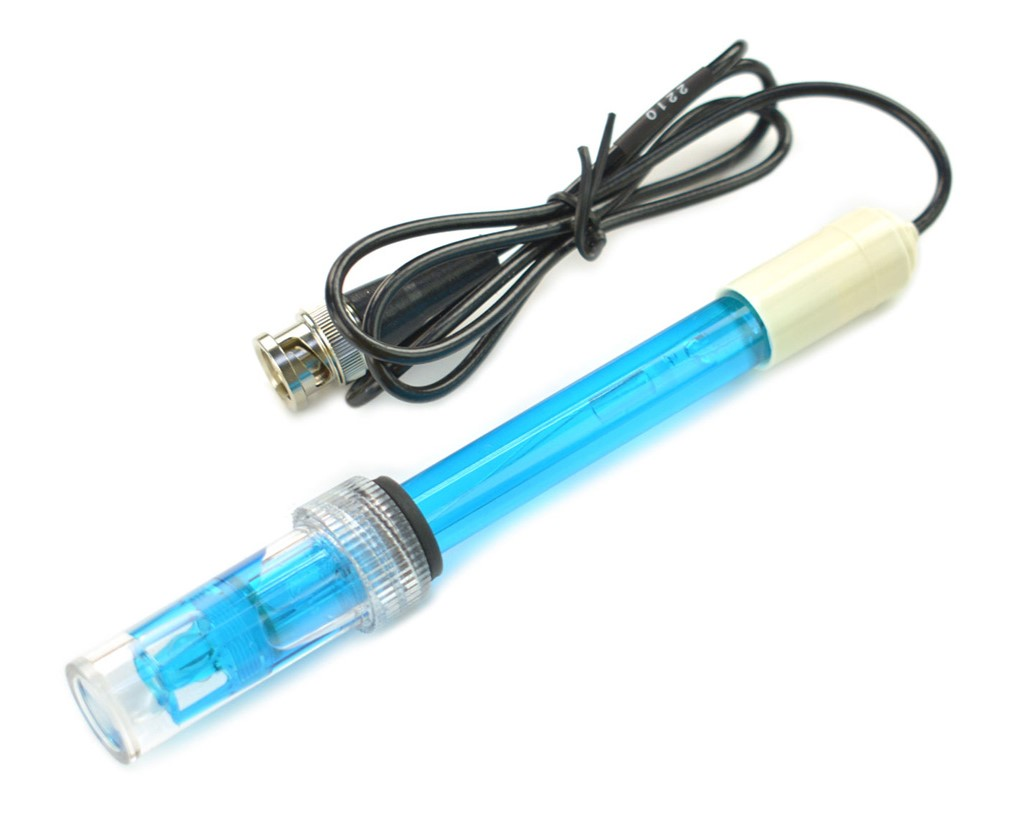
\includegraphics[width=1\linewidth]{Documento/Imagenes/Análisis/sensores/pH_sensor.jpg}}
    & \shortstack{\\ 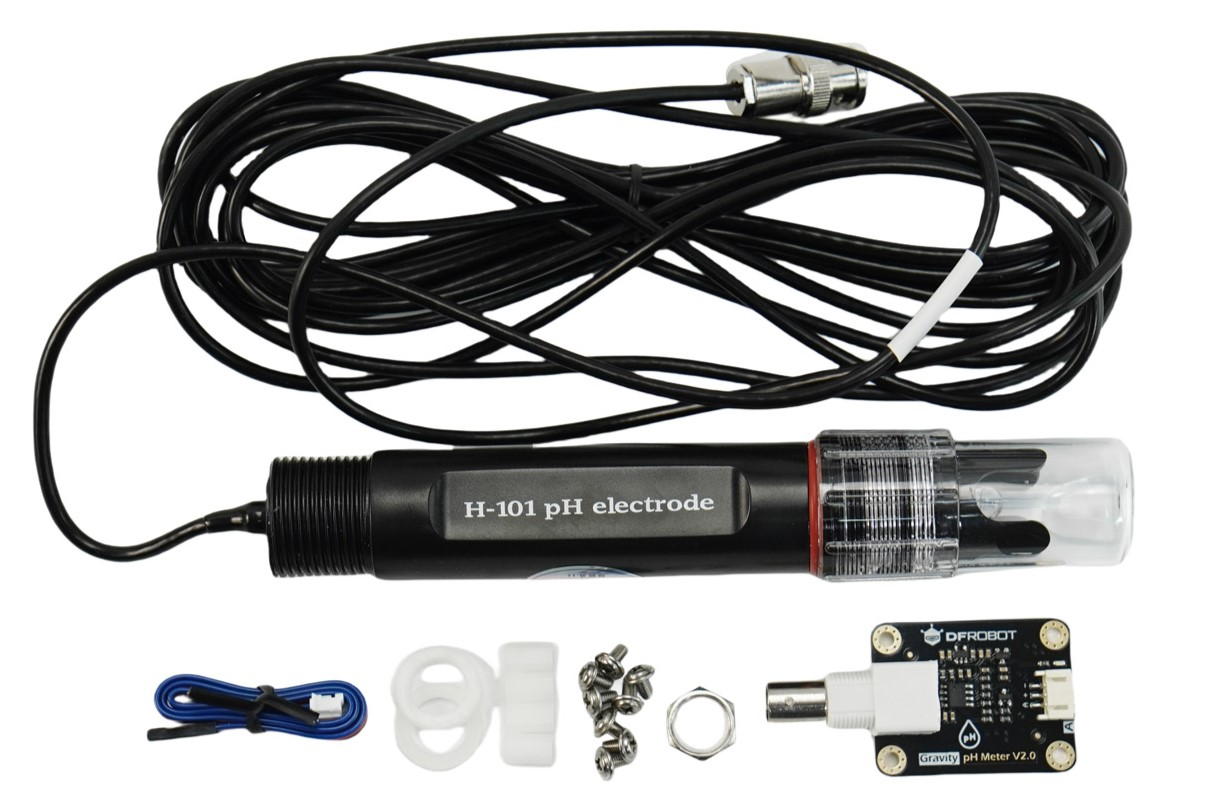
\includegraphics[width=1\linewidth]{Documento/Imagenes/Análisis/sensores/pH pro sensor.jpg}}
    & \shortstack{\\ 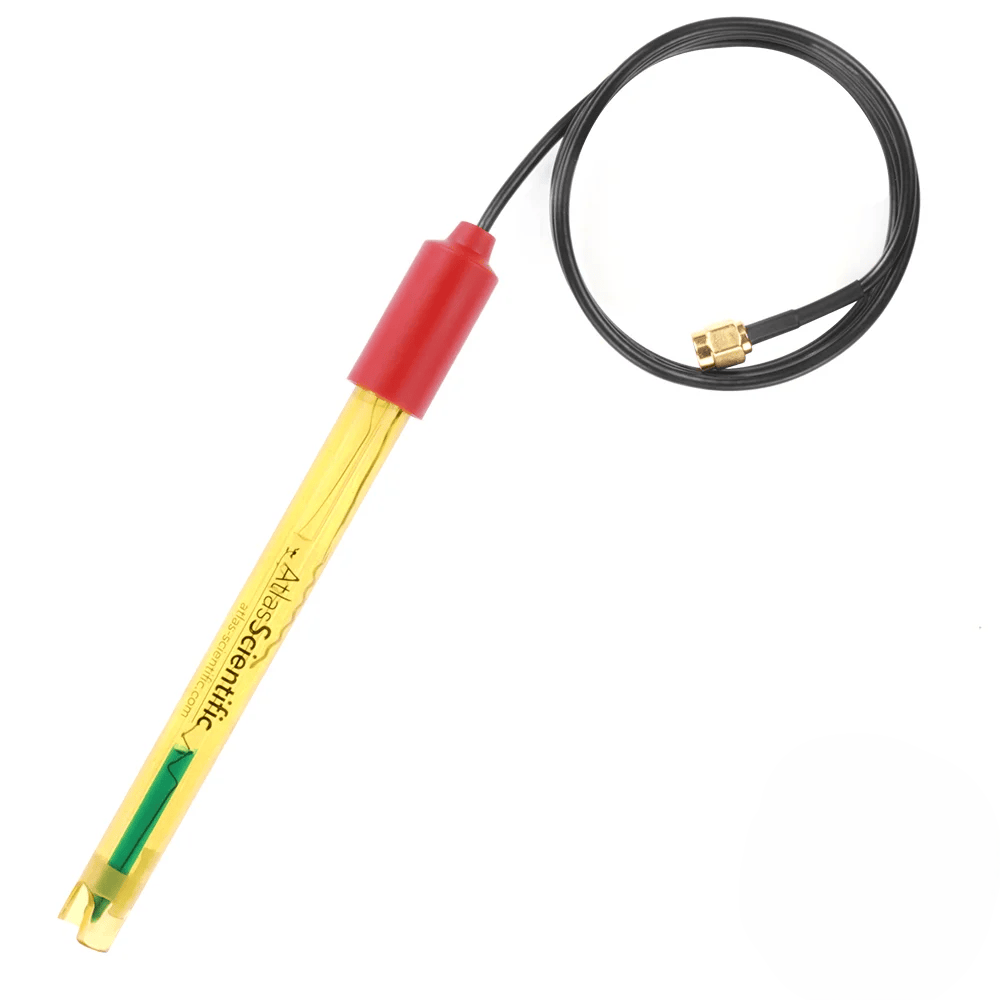
\includegraphics[width=1\linewidth]{Documento/Imagenes/Análisis/sensores/ph atlas sensor.png}} \\ \hline

\end{longtable}

Para la medición de pH, se han considerado dos alternativas principales de sensores de la línea Gravity de DFRobot: el \textit{Analog pH Meter V2} y el \textit{Industrial Analog pH Meter Pro Kit V2}. Ambos dispositivos ofrecen un rango de medición de 0 a 14 pH y una precisión de $\pm$0.1 pH a 25°C, con salidas analógicas compatibles con microcontroladores basados en ESP32.

La elección definitiva entre estos sensores dependerá de la evaluación del entorno específico donde se implementará el sistema. El \textit{Analog pH Meter V2} constituye una opción económica y de fácil integración, adecuada para aplicaciones en condiciones controladas o de baja exigencia ambiental. Por su parte, el \textit{Industrial Analog pH Meter Pro Kit V2} presenta características superiores para monitoreo continuo en ambientes hostiles, como un cable de sonda de 5 metros, un diseño robusto de grado industrial y una mayor resistencia a la exposición prolongada.

Considerando que el proyecto contempla la instalación de sensores en cuerpos de agua lóticos, donde se enfrentan condiciones variables de corriente y turbidez, el \textit{Industrial Analog pH Meter Pro Kit V2} se perfila como la opción más adecuada. No obstante, la selección final será confirmada tras la validación de las condiciones ambientales específicas del sitio de prueba.

%%%%%%%%%%%%%%%%%%%%%%%%%%%%%%%%%%%%%%%%%%%%%%%%%%%%
%             SECCIÓN: Oxigeno Disuelto            %
%%%%%%%%%%%%%%%%%%%%%%%%%%%%%%%%%%%%%%%%%%%%%%%%%%%%

\subsection{Análisis sensores oxigeno disuelto}
\renewcommand{\arraystretch}{1.5}
\begin{longtable}{
    |p{4cm}
    |p{5cm}
    |p{5cm}|
}
\caption{Comparativa de sensores para medición de oxígeno disuelto.}
\label{tab:sensores_od} \\
\hline
\textbf{Característica} 
    & \textbf{Gravity: Analog Dissolved Oxygen Sensor (SEN0237) \cite{DFRobot_DO_Sensor}} 
    & \textbf{Atlas Scientific EZO-DO™ \cite{Atlas_DO_Sensor_Manual}} \\
\hline
\endfirsthead

\hline
\textbf{Característica} 
    & \textbf{Gravity: Analog Dissolved Oxygen Sensor (SEN0237) \cite{DFRobot_DO_Sensor}} 
    & \textbf{Atlas Scientific EZO-DO™ \cite{Atlas_DO_Sensor_Manual}} \\
\hline
\endhead

\hline
\multicolumn{3}{r}{\textit{Continúa en la siguiente página}} \\
\endfoot

\hline
\endlastfoot

Tipo de tecnología 
    & Galvánica 
    & Óptica \\ \hline

Rango de medición 
    & 0--20 mg/L 
    & 0--50 mg/L \\ \hline

Precisión 
    & $\pm$0.2 mg/L 
    & $\pm$0.05 mg/L \\ \hline

Tipo de salida 
    & Analógica (0--3.0 V) 
    & UART / I2C / Analógica \\ \hline

Voltaje de operación 
    & 3.3--5.5 V 
    & 3.3--5.5 V \\ \hline

Compatibilidad con ESP32 
    & Sí (ADC) 
    & Sí (UART/I2C/ADC) \\ \hline

Diseñado para monitoreo continuo 
    & No recomendado 
    & Sí \\ \hline

Vida útil de la sonda 
    & 6--12 meses 
    & $>$2 años \\ \hline

Calibración necesaria 
    & Frecuente 
    & Muy baja frecuencia \\ \hline

Costo aproximado 
    & \$169 USD 
    & \$195+ USD \\ \hline

Ventajas 
    & Bajo costo, fácil de usar 
    & Alta precisión, mínima deriva, muy estable \\ \hline

Desventajas 
    & Afectado por temperatura y flujo, no ideal para monitoreo 24/7 
    & Muy costoso, integración más compleja \\ \hline

Imagen
    & \shortstack{\\ 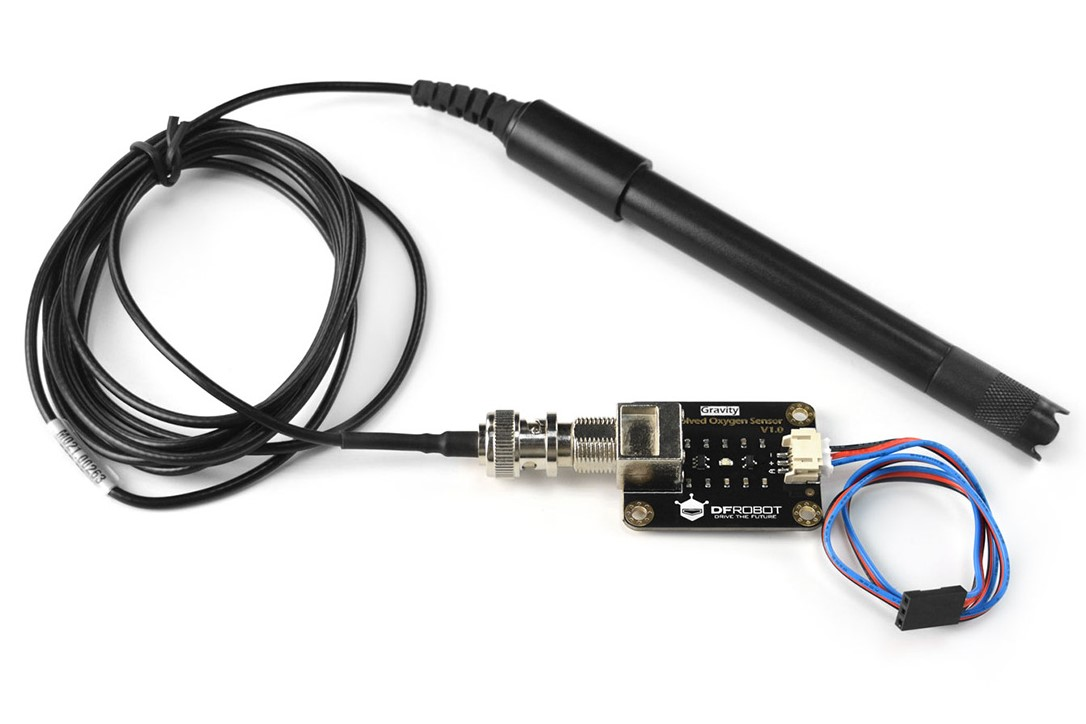
\includegraphics[width=0.8\linewidth]{Documento/Imagenes/Análisis/sensores/OD sensor.jpg}}
    & \shortstack{\\ 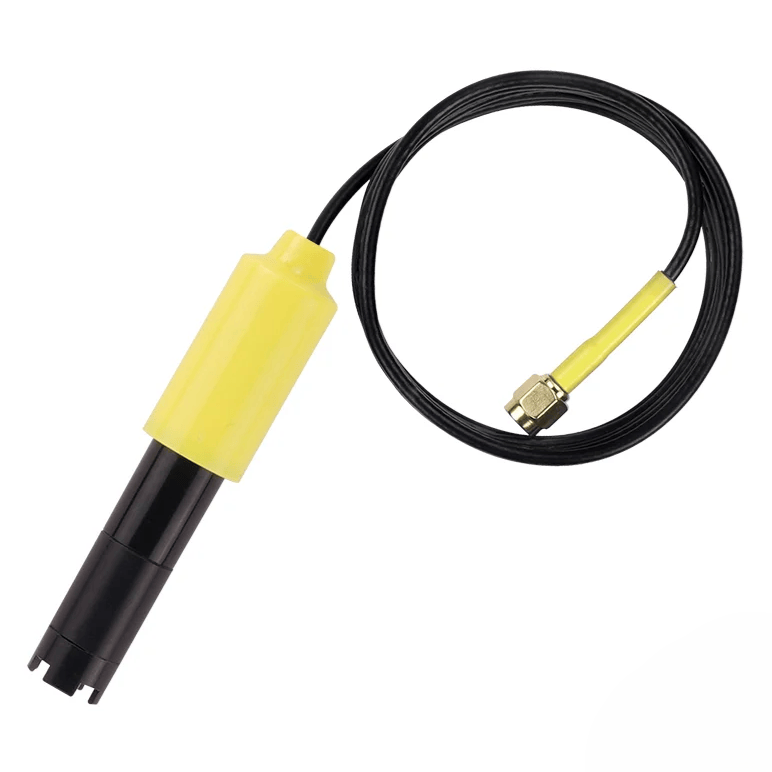
\includegraphics[width=0.8\linewidth]{Documento/Imagenes/Análisis/sensores/OD Atlas Sensor.png}} \\ \hline

\end{longtable}


Para la medición de oxígeno disuelto (OD) en el agua, se consideran dos opciones principales: el sensor Gravity: Analog Dissolved Oxygen Sensor (SEN0237) de DFRobot y el Atlas Scientific EZO-DO™.

El sensor Gravity Analog es una opción de bajo costo, basado en tecnología galvánica, que ofrece un rango de medición de 0 a 20 mg/L con una precisión de aproximadamente $\pm$0.2 mg/L. Su salida analógica facilita la integración con microcontroladores basados en ESP32. No obstante, presenta ciertas limitaciones para monitoreo continuo, ya que sufre interferencias por temperatura y flujo, y requiere calibraciones más frecuentes.

Por otro lado, el sensor Atlas Scientific EZO-DO™ utiliza tecnología óptica, ofreciendo un rango extendido de 0 a 50 mg/L y una alta precisión de $\pm$0.05 mg/L. Además, es adecuado para operaciones de monitoreo continuo en ambientes variables, con una mínima necesidad de calibración y una vida útil superior a los dos años. Sin embargo, su costo significativamente más elevado y su integración más compleja deben ser considerados.

Debido a que el sistema propuesto busca un equilibrio entre costos razonables y confiabilidad operativa, el sensor Gravity Analog se perfila como la opción más viable para su implementación inicial. No obstante, se mantiene abierta la posibilidad de considerar el sensor Atlas Scientific EZO-DO™ en futuras fases de ampliación o mejora del sistema, en caso de que se requiera una mayor precisión y robustez frente a condiciones ambientales extremas.

%%%%%%%%%%%%%%%%%%%%%%%%%%%%%%%%%%%%%%%%%%%%%%%%%%%%
%             SECCIÓN: Turbidez                    %
%%%%%%%%%%%%%%%%%%%%%%%%%%%%%%%%%%%%%%%%%%%%%%%%%%%%

\subsection{Análisis sensor de turbidez}
\renewcommand{\arraystretch}{1.5}
\begin{longtable}{
    |p{4cm}
    |p{8cm}|
}
\caption{Características del sensor seleccionado para la medición de turbidez.}
\label{tab:sensor_turbidez} \\
\hline
\textbf{Característica} 
    & \textbf{Gravity: Analog Turbidity Sensor (SEN0189) \cite{DFRobot_Turbidity_Sensor}} \\ 
\hline
\endfirsthead

\hline
\textbf{Característica} 
    & \textbf{Gravity: Analog Turbidity Sensor (SEN0189) \cite{DFRobot_Turbidity_Sensor}} \\ 
\hline
\endhead

\hline
\multicolumn{2}{r}{\textit{Continúa en la siguiente página}} \\
\endfoot

\hline
\endlastfoot

Tipo de tecnología 
    & Sensor óptico infrarrojo (dispersión de luz) \\ \hline

Rango de medición 
    & 0--1000 NTU \\ \hline

Precisión 
    & Dependiente de la calibración (aproximada) \\ \hline

Tipo de salida 
    & Analógica (0--4.5 V) \\ \hline

Voltaje de operación 
    & 5 V \\ \hline

Compatibilidad con ESP32 
    & Sí (entrada ADC) \\ \hline

Diseñado para monitoreo continuo 
    & No recomendado (sellado básico) \\ \hline

Vida útil de la sonda 
    & 6--12 meses (dependiendo de condiciones ambientales) \\ \hline

Calibración necesaria 
    & Frecuente en ambientes exteriores \\ \hline

Costo aproximado 
    & \$10 USD \\ \hline

Ventajas 
    & Bajo costo, fácil de usar, rápida integración \\ \hline

Desventajas 
    & Precisión limitada, sensibilidad a suciedad y humedad \\ \hline

Imagen
    & \shortstack{\\ 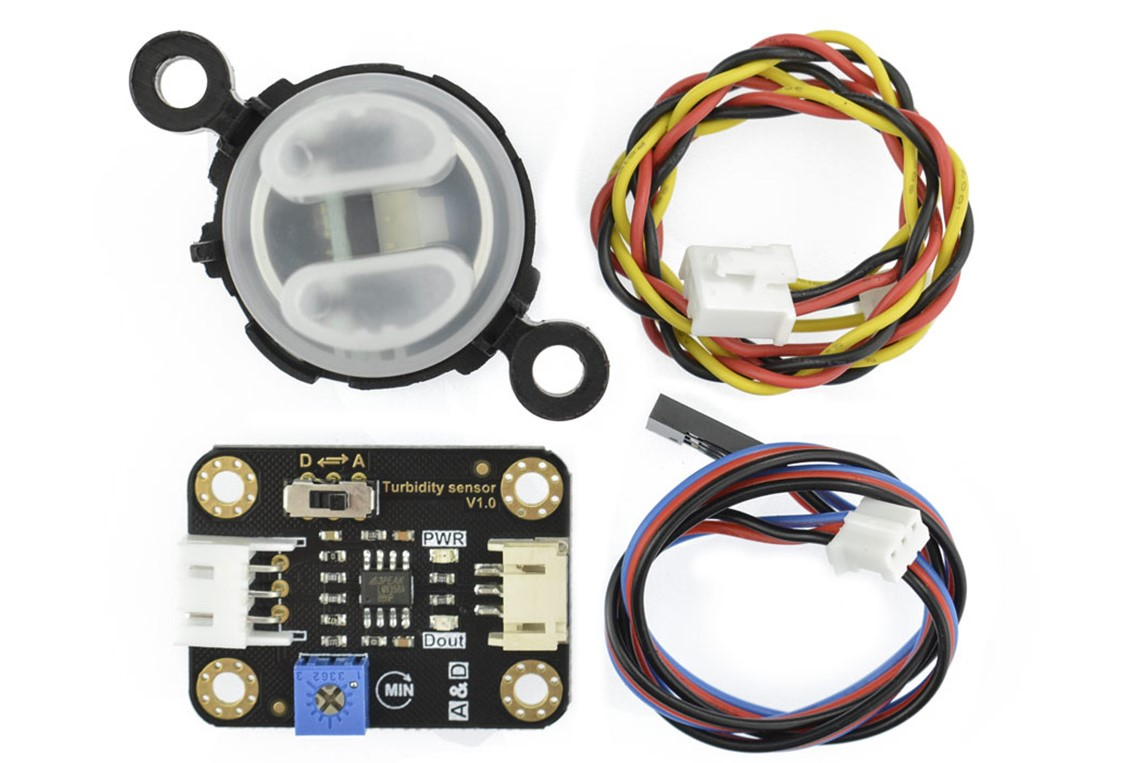
\includegraphics[width=0.7\linewidth]{Documento/Imagenes/Análisis/sensores/turbidez sensor.jpg}} \\ \hline

\end{longtable}


Para la medición de turbidez en el sistema propuesto se ha seleccionado el sensor Gravity: Analog Turbidity Sensor (SKU: SEN0189) de DFRobot. Este sensor permite medir niveles de turbidez en un rango de 0 a 1000 NTU, entregando una señal analógica proporcional a la concentración de partículas suspendidas en el agua. Su compatibilidad con microcontroladores basados en ESP32, su facilidad de integración mediante conversión analógica lo hacen adecuado para el presente proyecto.

Aunque su precisión es limitada en comparación con sensores digitales o de grado industrial, y su desempeño puede verse afectado por condiciones extremas de suciedad o humedad prolongada, su bajo costo y facilidad de implementación representan una alternativa viable para una primera fase de monitoreo distribuido en cuerpos de agua lóticos. La utilización de este sensor permitirá realizar una estimación práctica del nivel de sólidos suspendidos en el agua y, de ser necesario, futuras iteraciones del sistema podrán contemplar la adopción de tecnologías más robustas.

%%%%%%%%%%%%%%%%%%%%%%%%%%%%%%%%%%%%%%%%%%%%%%%%%%%%
%             SECCIÓN: Conductividad               %
%%%%%%%%%%%%%%%%%%%%%%%%%%%%%%%%%%%%%%%%%%%%%%%%%%%%

\subsection{Análisis sensores conductividad}
\renewcommand{\arraystretch}{1.5}
\begin{longtable}{
    |p{4cm}
    |p{5cm}
    |p{5cm}|
}
\caption{Comparativa de sensores para medición de conductividad eléctrica.}
\label{tab:sensor_conductividad} \\
\hline
\textbf{Característica} 
    & \textbf{Gravity: Analog EC Sensor V2 (DFR0300) \cite{DFRobot_EC_Sensor}} 
    & \textbf{Atlas Scientific EZO-EC™ \cite{AtlasScientific_Conductivity}} \\ 
\hline
\endfirsthead

\hline
\textbf{Característica} 
    & \textbf{Gravity: Analog EC Sensor V2 (DFR0300) \cite{DFRobot_EC_Sensor}} 
    & \textbf{Atlas Scientific EZO-EC™ \cite{AtlasScientific_Conductivity}} \\ 
\hline
\endhead

\hline
\multicolumn{3}{r}{\textit{Continúa en la siguiente página}} \\
\endfoot

\hline
\endlastfoot

Tipo de tecnología 
    & Electrodos de conductividad (K=1.0) 
    & Electrodos de conductividad \\ \hline

Parámetro principal 
    & Conductividad (EC) 
    & Conductividad (EC) \\ \hline

Rango de medición 
    & 0--20,000~$\mu$S/cm 
    & 0--200,000~$\mu$S/cm \\ \hline

Precisión 
    & $\pm$5\% F.S. 
    & $\pm$2\% F.S. \\ \hline

Tipo de salida 
    & Analógica (0--3.0 V) 
    & UART / I2C / Analógica \\ \hline

Voltaje de operación 
    & 3.0--5.0 V 
    & 3.3--5.5 V \\ \hline

Compatibilidad con ESP32 
    & Sí (ADC) 
    & Sí (UART/I2C/ADC) \\ \hline

Diseñado para monitoreo continuo 
    & Sí (recalibración periódica requerida) 
    & Sí (mínimo mantenimiento) \\ \hline

Vida útil de la sonda 
    & 6--12 meses 
    & $>$2 años \\ \hline

Calibración necesaria 
    & Periódica (solución estándar de conductividad) 
    & Muy baja frecuencia \\ \hline

Costo aproximado 
    & \$70 USD 
    & \$200+ USD \\ \hline

Ventajas 
    & Buen rango, estable, económico 
    & Alta precisión, muy robusto \\ \hline

Desventajas 
    & Requiere calibración manual periódica 
    & Alto costo, integración más compleja \\ \hline

Imagen
    & \shortstack{\\ 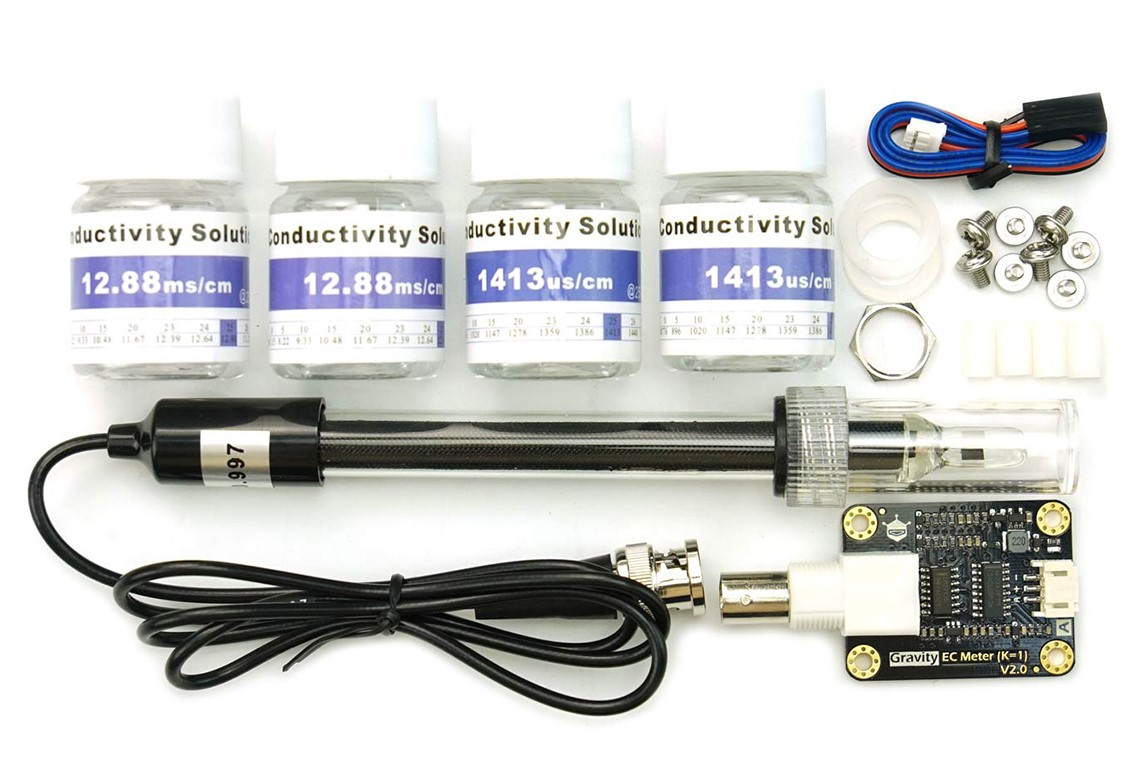
\includegraphics[width=0.8\linewidth]{Documento/Imagenes/Análisis/sensores/conductividad sensor.jpg}}
    & \shortstack{\\ 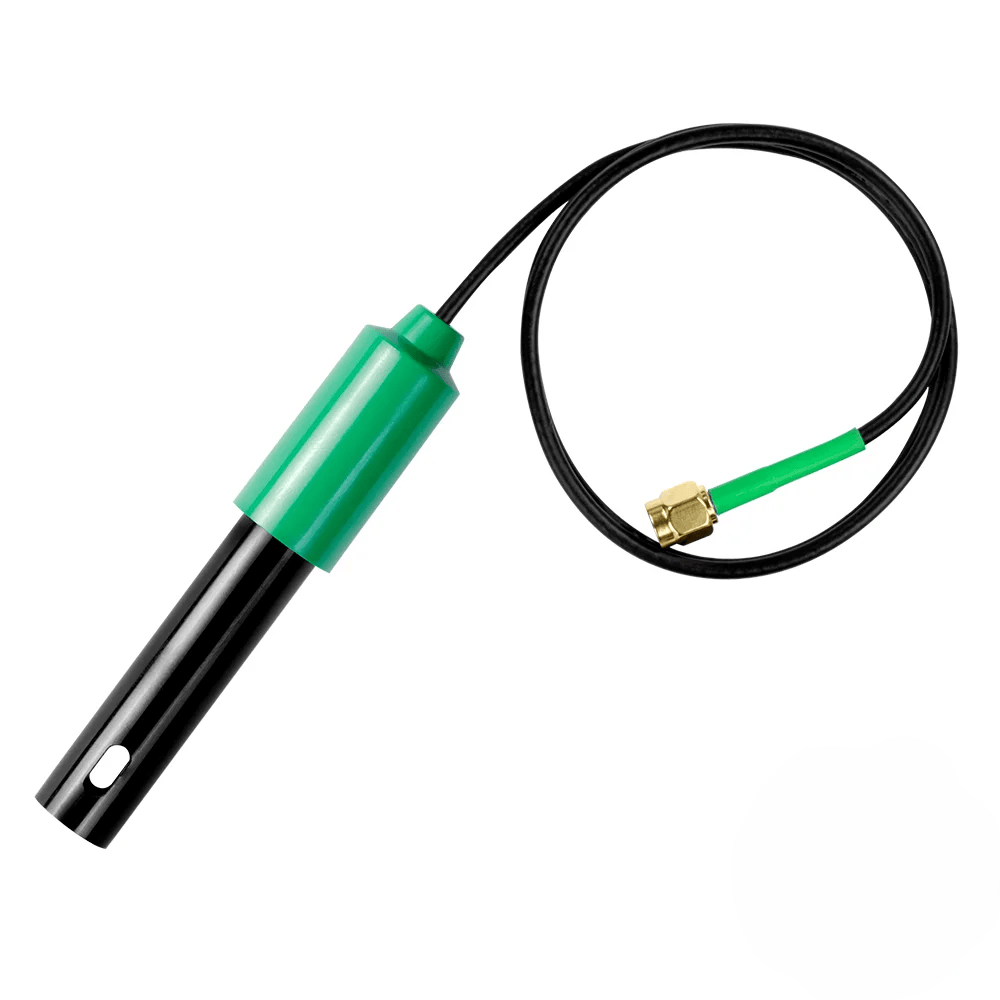
\includegraphics[width=0.8\linewidth]{Documento/Imagenes/Análisis/sensores/conductividad atlas sensor.png}} \\ \hline

\end{longtable}


Para la medición de conductividad eléctrica (EC) en el sistema propuesto se consideraron dos opciones: el sensor Gravity: Analog Electrical Conductivity Sensor V2 (SKU: DFR0300) de DFRobot y el Atlas Scientific EZO-EC™.

El sensor Gravity EC V2 ofrece un rango de medición de 0 a 20 mS/cm, con una precisión de $\pm$5\% de la escala completa. Su salida analógica facilita la integración directa con microcontroladores basados en ESP32, mediante el uso del convertidor analógico-digital (ADC) interno. Además, su costo accesible y su diseño robusto lo convierten en una opción viable para proyectos de monitoreo distribuido en cuerpos de agua lóticos. No obstante, requiere calibraciones periódicas utilizando soluciones estándar de conductividad, especialmente en aplicaciones de largo plazo.

En contraste, el sensor Atlas Scientific EZO-EC™ proporciona un rango extendido de hasta 200 mS/cm, alta precisión de $\pm$2\%, y mínimas necesidades de calibración. Sin embargo, su costo elevado y su integración más compleja lo hacen menos accesible para un sistema que busca un equilibrio entre funcionalidad y viabilidad económica.

Considerando los objetivos de este Proyecto y las restricciones presupuestarias, se selecciona el sensor Gravity: Analog Electrical Conductivity Sensor V2 como la opción más adecuada para la medición de conductividad, dejando abierta la posibilidad de futuras mejoras en etapas posteriores del proyecto.
%%%%%%%%%%%%%%%%%%%%%%%%%%%%%%%%%%%%%%%%%%%%%%%%%%%%
%             SECCIÓN: Temperatura                 %
%%%%%%%%%%%%%%%%%%%%%%%%%%%%%%%%%%%%%%%%%%%%%%%%%%%%

\subsection{Análisis sensores temperatura}
\renewcommand{\arraystretch}{1.5}
\begin{longtable}{
    |p{4cm}
    |p{5cm}
    |p{5cm}|
}
\caption{Comparativa de sensores para medición de temperatura.}
\label{tab:sensor_temperatura} \\
\hline
\textbf{Característica} 
    & \textbf{DS18B20 Sumergible \cite{DFRobot_DS18B20}} 
    & \textbf{Atlas Scientific EZO-RTD™ \cite{Atlas_EZO_RTD}} \\ 
\hline
\endfirsthead

\hline
\textbf{Característica} 
    & \textbf{DS18B20 Sumergible \cite{DFRobot_DS18B20}} 
    & \textbf{Atlas Scientific EZO-RTD™ \cite{Atlas_EZO_RTD}} \\ 
\hline
\endhead

\hline
\multicolumn{3}{r}{\textit{Continúa en la siguiente página}} \\
\endfoot

\hline
\endlastfoot

Tipo de tecnología 
    & Sensor digital 1-Wire 
    & RTD PT-1000 industrial \\ \hline

Rango de medición 
    & -55\,\textdegree C a +125\,\textdegree C 
    & -200\,\textdegree C a +850\,\textdegree C \\ \hline

Precisión típica 
    & $\pm$0.5\,\textdegree C (-10\,\textdegree C a +85\,\textdegree C) 
    & $\pm$0.1\,\textdegree C \\ \hline

Tipo de salida 
    & Digital (1-Wire) 
    & UART / I2C \\ \hline

Voltaje de operación 
    & 3.0--5.5 V 
    & 3.3--5.5 V \\ \hline

Compatibilidad con ESP32 
    & Sí (1-Wire) 
    & Sí (UART/I2C) \\ \hline

Diseñado para inmersión continua 
    & Sí 
    & Sí \\ \hline

Calibración necesaria 
    & No 
    & No \\ \hline

Costo aproximado 
    & \$7.5 USD 
    & \$30 USD \\ \hline

Ventajas 
    & Muy económico, fácil integración, adecuado para monitoreo de calidad de agua 
    & Altísima precisión, robustez industrial \\ \hline

Desventajas 
    & Menor precisión que RTD, rango limitado para aplicaciones extremas 
    & Alto costo, integración más compleja \\ \hline

Imagen
    & \shortstack{\\ 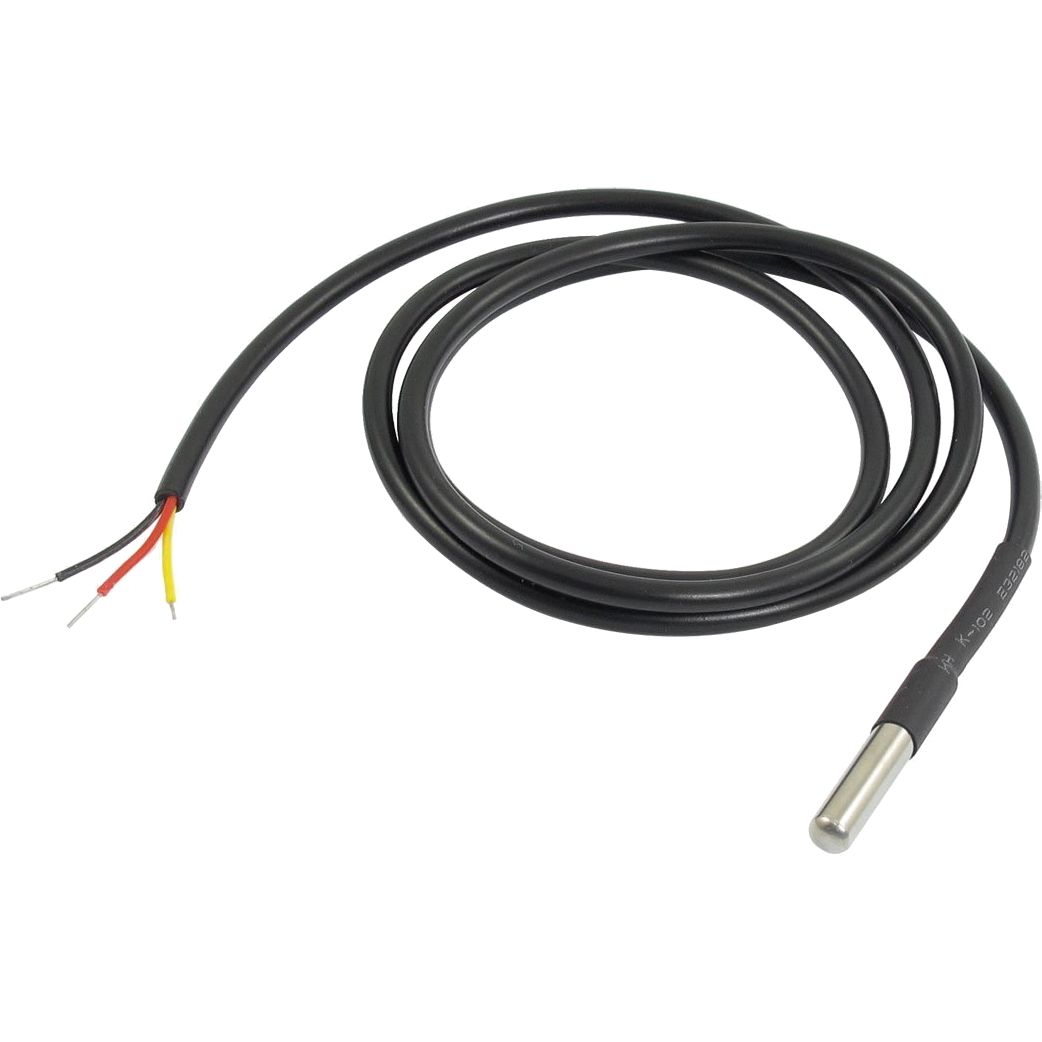
\includegraphics[width=0.75\linewidth]{Documento/Imagenes/Análisis/sensores/Temp_Sensor.png}}
    & \shortstack{\\ 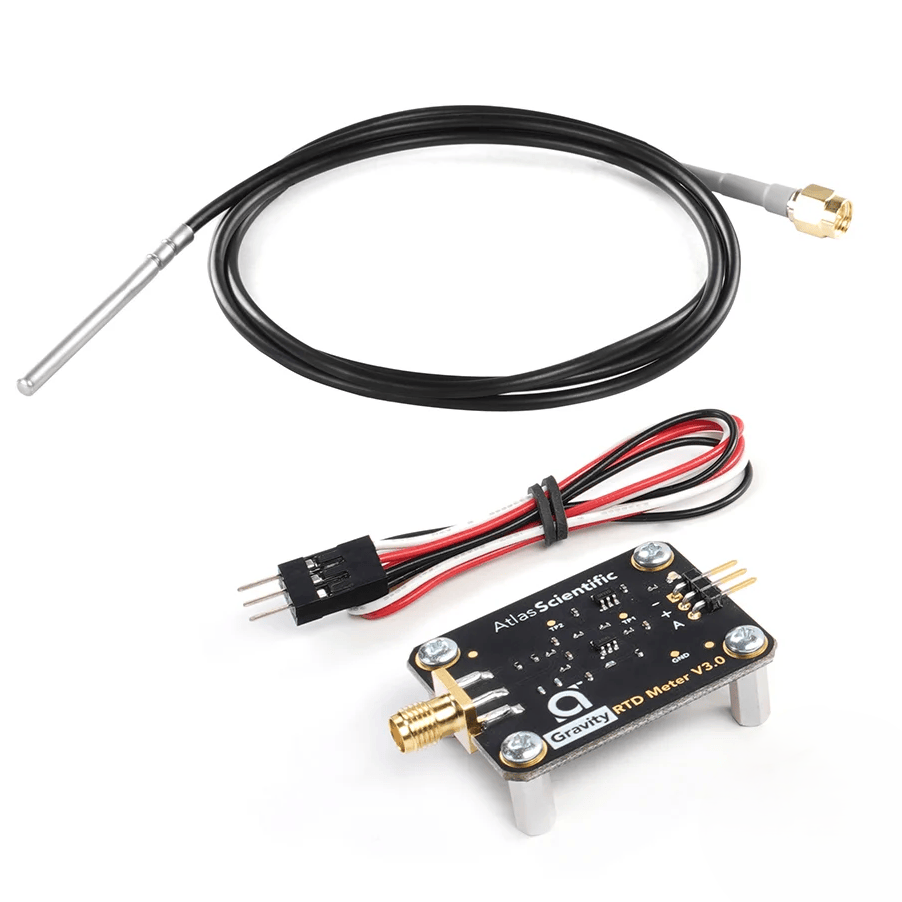
\includegraphics[width=0.75\linewidth]{Documento/Imagenes/Análisis/sensores/Temp_Atlas_Sensor.png}} \\ \hline

\end{longtable}


Para la medición de temperatura en el sistema propuesto se consideraron dos alternativas: el sensor digital sumergible DS18B20 y el sensor industrial Atlas Scientific EZO-RTD™.

El sensor DS18B20, ampliamente utilizado en aplicaciones de monitoreo ambiental, ofrece un rango de medición de -55°C a 125°C con una precisión típica de ±0.5°C en el rango de -10°C a 85°C. Su comunicación mediante el protocolo digital 1-Wire facilita su integración directa con microcontroladores basados en ESP32. Además, su bajo costo, facilidad de adquisición y resistencia a la inmersión continua en agua lo convierten en una opción práctica y adecuada para sistemas de monitoreo distribuidos en cuerpos de agua.

Por su parte, el sensor Atlas Scientific EZO-RTD™ proporciona una mayor precisión (±0.1°C) y un rango de operación mucho más amplio, gracias al uso de sensores RTD de tipo PT-1000. Sin embargo, su alto costo y mayor complejidad de integración lo hacen menos adecuado para proyectos donde se busca un balance entre funcionalidad y viabilidad económica.

Considerando los objetivos de este Proyecto y las condiciones operativas previstas, se selecciona el sensor DS18B20 sumergible como la opción más adecuada para la medición de temperatura en cuerpos de agua lóticos.

%%%%%%%%%%%%%%%%%%%%%%%%%%%%%%%%%%%%%%%%%%%%%%%%%%%%
%             SECCIÓN: Topologia de red            %
%%%%%%%%%%%%%%%%%%%%%%%%%%%%%%%%%%%%%%%%%%%%%%%%%%%%

\section{Análisis de la topología de red}


El diseño de la Red Inalámbrica de Sensores (WSN) es fundamental para garantizar la conectividad fiable y eficiente entre los nodos distribuidos y el sistema central de procesamiento. Para este proyecto, se ha seleccionado una \textbf{topología lineal multisalto} (\textit{multi-hop linear topology}).

\subsection{Descripción de la Topología Seleccionada}
\label{subsec:descripcion_topologia}

La red se compone de cuatro nodos sensores (N=4) desplegados secuencialmente a lo largo del cuerpo de agua lótico y un nodo final denominado nodo concentrador o \textit{gateway} (\textit{sink node}), ubicado al final de la cadena. Cada nodo sensor ($n=1, ..., 4$) captura datos fisicoquímicos e imágenes. La comunicación hacia el \textit{gateway} se realiza mediante un esquema de retransmisión secuencial (\textit{store-and-forward}), donde cada nodo $n$ recibe los datos acumulados de los nodos $1$ a $n-1$ y los retransmite junto con sus propios datos hacia el nodo $n+1$ (o hacia el \textit{gateway} si $n=N$). La Figura \ref{fig:topologia_lineal_fluvial} ilustra esta configuración.

\begin{figure}[H]
   \centering
   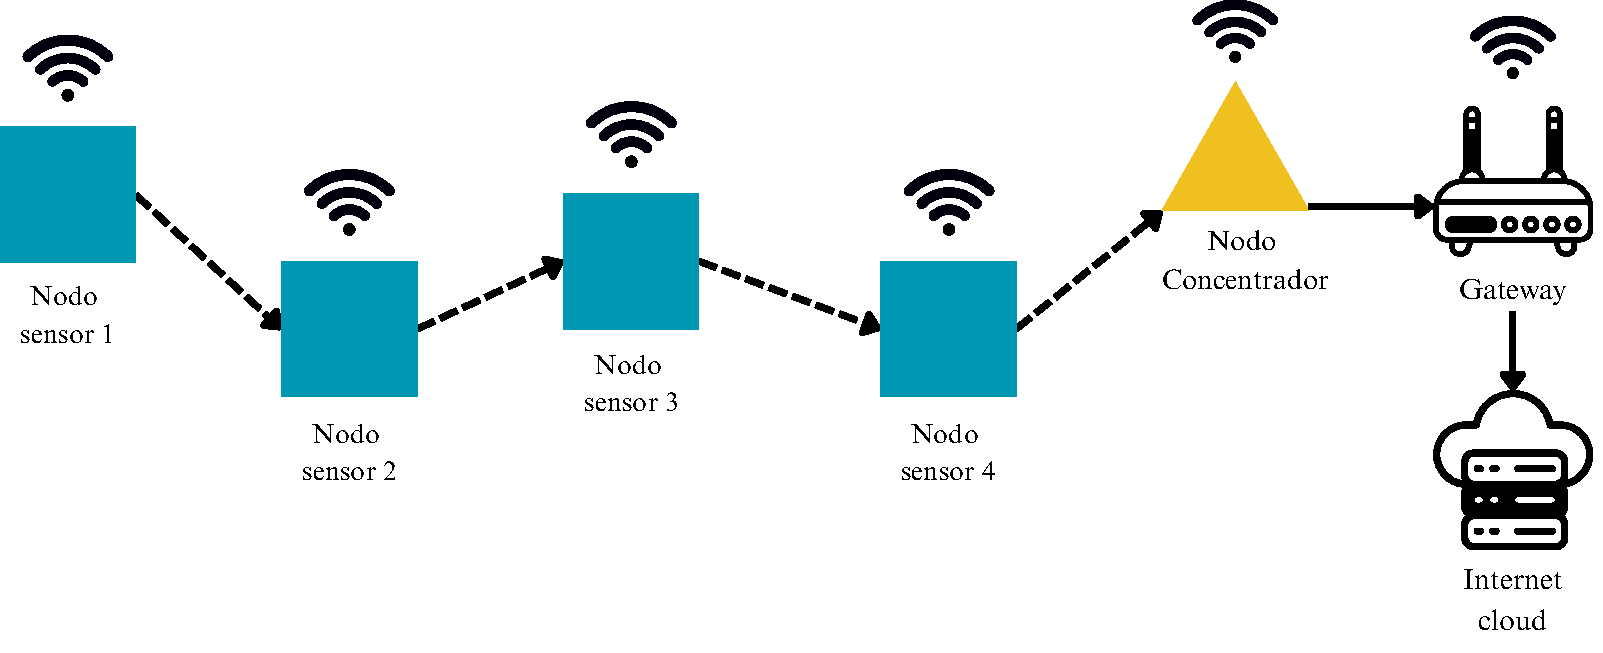
\includegraphics[width=0.8\linewidth]{Documento/Imagenes/Análisis/Topologia/Topologia_Lineal.pdf}
   \caption{Topología lineal multisalto para el monitoreo fluvial. Los nodos sensores se comunican mediante enlaces inalámbricos (líneas discontinuas), y el Nodo Sink/Gateway se conecta a la nube mediante Wi-Fi estándar (línea sólida).}
   \label{fig:topologia_lineal_fluvial}
\end{figure}

El \textit{gateway} actúa como punto de agregación final. Recibe toda la información de la WSN a través del enlace inalámbrico proveniente del último nodo sensor (Nodo 4). Posteriormente, utiliza una interfaz de comunicación distinta, Wi-Fi estándar (IEEE 802.11n/g), para transmitir los datos consolidados al servidor central alojado en la nube. Esta elección para el enlace final (\textit{backhaul}) facilita la integración con infraestructuras de red comunes (routers Wi-Fi) para el acceso a Internet.


\subsection{Justificación de la Topología Lineal}
\label{subsec:justificacion_topologia}

La topología lineal se considera la más adecuada para el monitoreo de entornos fluviales por las siguientes razones:

\begin{itemize}
    \item \textbf{Adaptación al Entorno Geográfico:} Se alinea de forma natural con la morfología alargada de ríos y arroyos.
    \item \textbf{Monitoreo Longitudinal:} Facilita el estudio de la evolución espacial de parámetros a medida que el agua fluye.
    \item \textbf{Simplicidad de Enrutamiento:} El flujo de datos es determinista (de $n$ a $n+1$), simplificando la lógica en los nodos y ahorrando energía al evitar protocolos de enrutamiento complejos. 
\end{itemize}
Alternativas como topologías en estrella o malla presentarían desventajas en términos de alcance o complejidad para esta aplicación específica.

\subsection{Esquema de Comunicación Inter-Nodo}
\label{subsec:esquema_comunicacion_inter_nodo} 

La comunicación \textit{entre} los nodos sensores y hacia el \textit{gateway} utilizará una tecnología inalámbrica de medio alcance y bajo consumo (cuya selección se detalla en la Sección \ref{sec:analisis_tecnologias}). Esta tecnología deberá operar en modo \textit{half-duplex}, lo cual impacta el tiempo total de comunicación, como se analizó en la Sección \ref{ssubsec:tiempo_general_comm}. El esquema de retransmisión es \textit{store-and-forward}, requiriendo mecanismos básicos de fiabilidad como confirmaciones de recepción (ACK) para asegurar la entrega entre saltos.

\subsection{Implicaciones Técnicas y Limitaciones}
\label{subsec:implicaciones_topologia}

La topología lineal seleccionada presenta ciertas implicaciones:

\begin{itemize}
    \item \textbf{Carga Energética Desbalanceada:} Los nodos más cercanos al \textit{gateway} (Nodo 4) soportan mayor tráfico de retransmisión (Ecuación \eqref{eq:tiempo_comm_nodo_n}), requiriendo un dimensionamiento energético cuidadoso.
    \item \textbf{Retardo Acumulado:} Tolerable dada la baja frecuencia de muestreo semanal.
    \item \textbf{Tolerancia a Fallos Limitada:} La falla de un nodo intermedio interrumpe la cadena. Se considerarán mecanismos de detección de fallos o redundancia para futuras fases.
\end{itemize}

A pesar de la limitación en la tolerancia a fallos, la simplicidad, eficiencia y adecuación geográfica de la topología lineal la validan como la opción más pragmática para la fase actual del proyecto. La conexión final del \textit{gateway} mediante Wi-Fi estándar simplifica la integración con la infraestructura de nube.



%%%%%%%%%%%%%%%%%%%%%%%%%%%%%%%%%%%%%%%%%%%%%%%%%%%%
%             SECCIÓN: Transceptores               %
%%%%%%%%%%%%%%%%%%%%%%%%%%%%%%%%%%%%%%%%%%%%%%%%%%%%

\section{Análisis de Transceptores Inalámbricos}
\label{sec:analisis_tecnologias}

Para seleccionar la tecnología más adecuada para la transmisión de datos en el sistema de monitoreo, se evaluaron distintos estándares inalámbricos considerando tres criterios fundamentales:

\begin{enumerate}
    \item \textbf{Consumo energético}: Factor determinante para asegurar una operación prolongada mediante baterías, minimizando la necesidad de mantenimiento.
    \item \textbf{Alcance efectivo}: Capacidad del protocolo para cubrir distancias en una topología lineal, considerando la presencia de obstáculos naturales como vegetación y accidentes geográficos.
    \item \textbf{Tasa máxima de transmisión}: Velocidad teórica máxima con la que se pueden enviar datos, clave para asegurar el envío oportuno de lecturas y archivos, como imágenes capturadas por el sistema.
\end{enumerate}

La Tabla~\ref{tab:redes_corto_alcance} presenta un resumen comparativo de soluciones de red de corto alcance comúnmente utilizadas en aplicaciones de monitoreo ambiental con WSN. Se incluyen tecnologías basadas en los estándares IEEE 802.15.4 y 802.15.1, como ZigBee, 6LoWPAN, Bluetooth y BLE, analizando sus tasas de transmisión, topologías soportadas, rango típico de cobertura, frecuencia de operación y consumo energético. Estas soluciones priorizan eficiencia energética y bajo costo de despliegue, aunque con limitaciones en velocidad o alcance.

\begin{table}[H]
\centering
\caption{Resumen de soluciones de red de corto alcance \cite{lopez2023}}
\label{tab:redes_corto_alcance}
\renewcommand{\arraystretch}{1.3}
\resizebox{\textwidth}{!}{
\begin{tabular}{p{2.5cm}p{2.5cm}p{2cm}p{2.5cm}p{2cm}p{1.5cm}p{2.3cm}}
\toprule
\textbf{Solution} & \textbf{Standard} & \textbf{Data rate} & \textbf{Coverage} & \textbf{Topology} & \textbf{Carrier freq} & \textbf{Energy cost} \\
\midrule
IEEE 802.15.4      & IEEE 802.15.4     & 250 kbps           & $<$100 m          & Star, tree, cluster tree, mesh & 868/915 MHz, 2.4 GHz & Low \\
ZigBee             & IEEE 802.15.4     & 250, 40, 20 kbps    & $>$100 m          & Mesh, star, tree               & 868/915 MHz, 2.4 GHz & Low \\
6LoWPAN            & IEEE 802.15.4     & 250 kbps           & $<$100 m          & Mesh, star                     & 868/915 MHz, 2.4 GHz & Low \\
Bluetooth          & IEEE 802.15.1     & 1 Mbps             & Up to 100 m       & Star, P2P                      & 2.4 GHz              & Low \\
BLE                & IEEE 802.15.1     & 1 Mbps             & Up to 200 m       & Star, P2P                      & 2.4 GHz              & Very low \\
\bottomrule
\end{tabular}
}
\end{table}

La Tabla~\ref{tab:redes_alcance_medio} complementa el análisis anterior al enfocarse en redes de alcance medio. Se comparan dos variantes del estándar IEEE 802.11: Wi-Fi tradicional y Wi-Fi HaLow (802.11ah). Aunque Wi-Fi convencional ofrece altas tasas de transferencia, su consumo energético es elevado y su cobertura limitada. En cambio, Wi-Fi HaLow opera en bandas sub-GHz, permitiendo mayor alcance, menor consumo y adecuada velocidad, lo que lo hace más apropiado para entornos remotos como cuerpos de agua lóticos.

\begin{table}[H]
\centering
\caption{Resumen de soluciones de red de alcance medio \cite{lopez2023}}
\label{tab:redes_alcance_medio}
\renewcommand{\arraystretch}{1.3}
\resizebox{\textwidth}{!}{
\begin{tabular}{p{2.5cm}p{2.5cm}p{2cm}p{2.5cm}p{2.5cm}p{1.5cm}p{2.3cm}}
\toprule
\textbf{Solution} & \textbf{Standard} & \textbf{Data rate} & \textbf{Coverage} & \textbf{Topology} & \textbf{Carrier freq} & \textbf{Energy cost} \\
\midrule
Wi-Fi & IEEE 802.11 & Up to 54 Mbps & 200 m & Infrastructure, mesh & 2.4 GHz, 5 GHz & High \\
Wi-Fi HaLow & IEEE 802.11ah   & 0.15 to 4 Mbps @ 1 MHz bandwidth, an 0.65 to 7.8 Mbps @ 2 MHz bandwidth & 1000m & star, mesh & ISM Sub-GHz & Low \\ 
\bottomrule
\end{tabular}
}
\end{table}

Dadas las posibles soluciones, en la Tabla~\ref{tab:comparativa_transceptores} se comparan módulos transceptores comerciales representativos de cada tecnología evaluada. Se contrastan parámetros clave como tasa máxima de transmisión, potencia de transmisión y sensibilidad de recepción, alcance en línea de vista (LOS), y consumo de corriente en modos activo y en reposo. 
\begin{table}[H]
\renewcommand{\arraystretch}{1.5}
\centering
\caption{Comparativa de transceptores comerciales para WSN}
\label{tab:comparativa_transceptores}
\resizebox{\textwidth}{!}{
\begin{tabular}{|p{3.2cm}|C{3cm}|C{3cm}|C{3cm}|C{3cm}|C{3cm}|}
\hline
\textbf{Parámetro} 
& \shortstack{\\ \textbf{Wi-Fi HaLow}\\ \textbf{(802.11ah)}} 
& \shortstack{\\ \textbf{Wi-Fi}\\ \textbf{(802.11n)}} 
& \shortstack{\\ \textbf{Zigbee}\\ \textbf{(802.15.4)}} 
& \shortstack{\\ \textbf{Bluetooth} \\ \textbf{(802.15.1)}}
& \shortstack{\\ \textbf{LoRaWAN}\\ \textbf{(P1451.5.5)}} \\ \hline

\textbf{Módulo} & FGH100M \cite{QuectelFGH100M} & ESP32-S3 \cite{EspressifESP32S3} & XBee S2C \cite{DigiXBeeS2C} & HC-05 \cite{HC05Datasheet} & Wio E5 LE \cite{SeeedWioE5LE} \\ \hline
\textbf{Tasa Máx. (Mbps)} & 32.5 & 150 & 0.25 & 2.1 & 0.05 \\ \hline
\textbf{Potencia Tx / Sensibilidad Rx (dBm)} & 20 / -98 & 19 / -75 & 5 / -100 & 4 / -84 & 13.461 / -137 \\ \hline
\textbf{Alcance LOS\footnote{Line Of Sight} (m)} & 1000 & 120 & 1200 & 40 & 10000 \\ \hline
\textbf{Consumo Tx (mA)} & 54 & 286 & 33 & 30 & 26 \\ \hline
\textbf{Consumo Rx (mA)} & 43 & 95 & 28 & 30 & 13 \\ \hline
\textbf{Consumo en Sleep (µA)} & TBD & 240 & 1 & TBD & 1.3 \\ \hline

\end{tabular}
}
\end{table}

Esta comparativa refuerza la selección de Wi-Fi HaLow mediante el módulo FGH100M, al ofrecer un equilibrio favorable entre alcance, velocidad, consumo y viabilidad de integración en nodos autónomos. En la tabla \ref{tab:imagenes_transceptore} se presentan imágenes representativas de cada transceptor evaluado para facilitar su identificación visual.


\begin{table}[H]
\renewcommand{\arraystretch}{1.5}
\centering
\caption{Ilustraciones transceptores}
\label{tab:imagenes_transceptore}
\resizebox{\textwidth}{!}{
\begin{tabular}{|C{3.5cm}|C{3.5cm}|C{3.5cm}|C{3.5cm}|C{3.5cm}|}
\hline
 \textbf{FGH100M} & \textbf{ESP32-S3} & \textbf{XBee S2C} & \textbf{HC-05} & \textbf{Wio E5 LE} \\ \hline

\shortstack{\\ 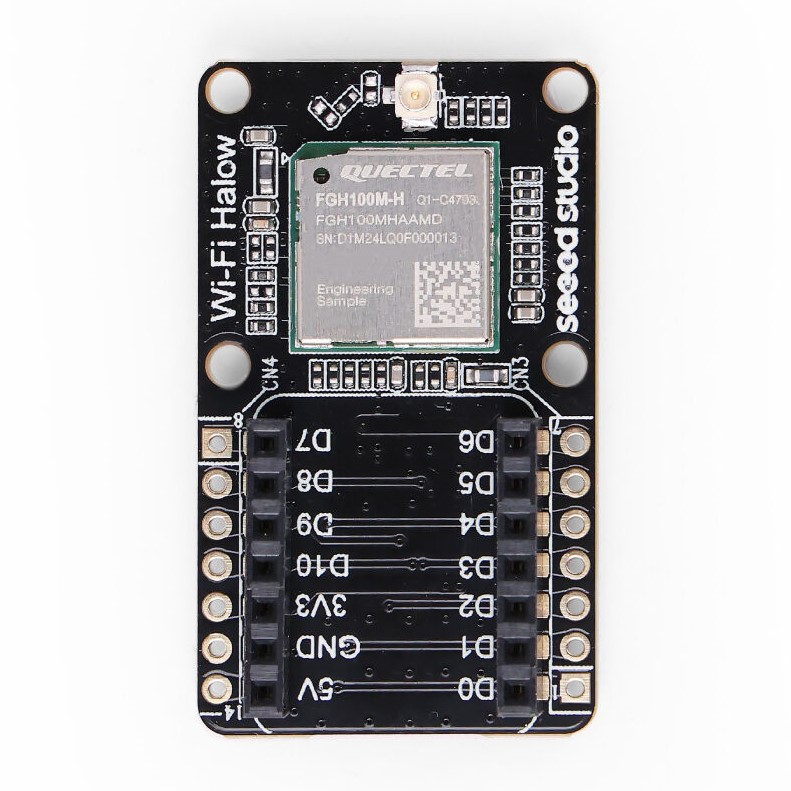
\includegraphics[width=1 \linewidth]{Documento/Imagenes/Análisis/Transceptores/Xiao Halow.jpg}}
&
\shortstack{\\ 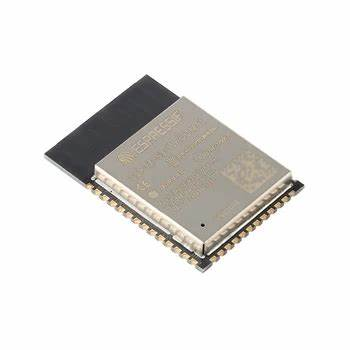
\includegraphics[width=1 \linewidth]{Documento/Imagenes/Análisis/Transceptores/Esp32.jpg}}
&
\shortstack{\\ 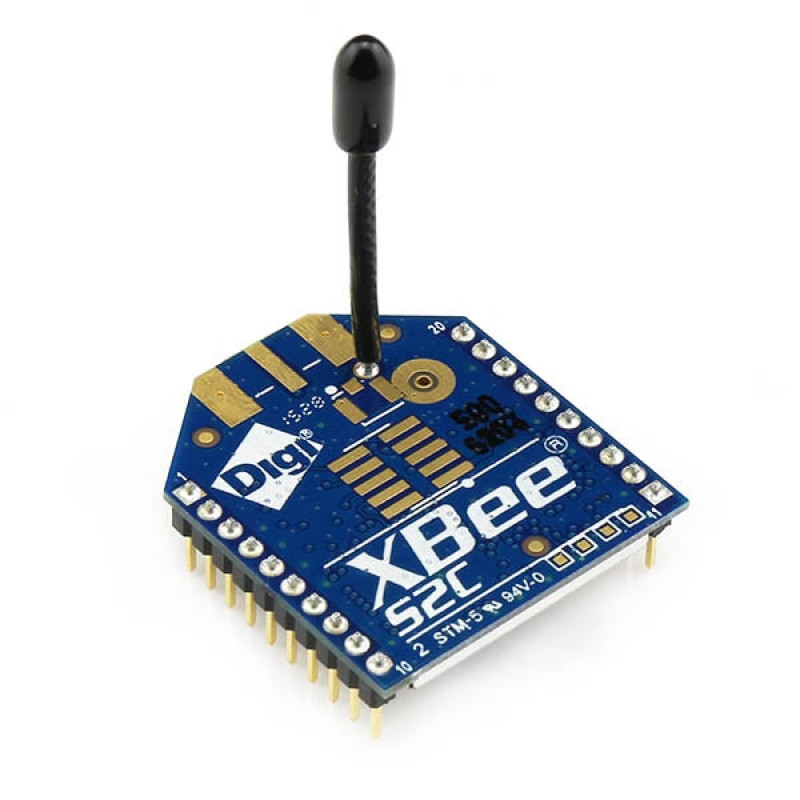
\includegraphics[width=1 \linewidth]{Documento/Imagenes/Análisis/Transceptores/zigbee.jpg}}
&
\shortstack{\\ 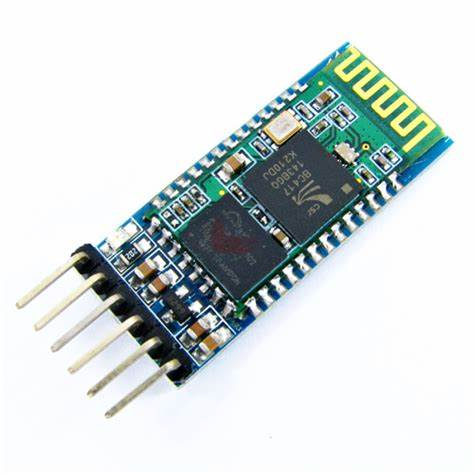
\includegraphics[width=1 \linewidth]{Documento/Imagenes/Análisis/Transceptores/HC-05.jpg}}
&
\shortstack{\\ 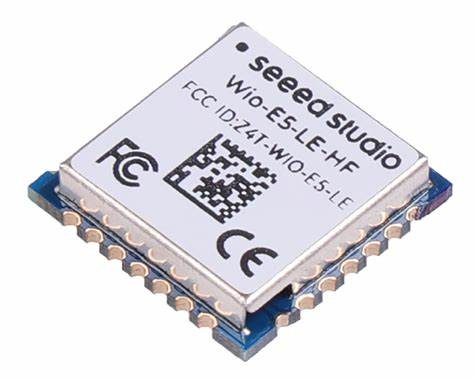
\includegraphics[width=1 \linewidth]{Documento/Imagenes/Análisis/Transceptores/Lorawan.jpg}}
\\ \hline
\end{tabular}
}
\end{table}


Como solución óptima para la transmisión bidireccional de los datos, en este caso, datos de los sensores e imagenes captadas en entornos fluviales, se propone el módulo FGH100M (Wi-Fi HaLow) como transceptor preliminar. Esta selección se fundamenta por su  exelente equilibrio entre alcance efectivo (1 km en condiciones ideales) y consumo energético moderado (54 mA en TX/43 mA en RX), características críticas para la operación prolongada en topologías lineales con nodos distribuidos. Su operación en banda sub-1 GHz (902-928 MHz) proporciona mayor penetración en vegetación ribereña comparado con soluciones en 2.4 GHz, manteniendo compatibilidad con el estándar IEEE 802.11ah para gestión adaptativa de energía mediante mecanismos TIM/RAW. Adicionalmente, soporta tasas de transferencia suficientes (32.5 Mbps) para la transmisión eficiente de datos sensoriales e imágenes comprimidas, cumpliendo con los requisitos de bidireccionalidad para recepción de comandos desde el servidor central.


%%%%%%%%%%%%%%%%%%%%%%%%%%%%%%%%%%%%%%%%%%%%%%%%%%%%
%             SECCIÓN: Cámaras                    %
%%%%%%%%%%%%%%%%%%%%%%%%%%%%%%%%%%%%%%%%%%%%%%%%%%%%
\section{Análisis de cámaras}

Para la selección de la cámara que formará parte del sistema de visión artificial, se evaluaron cuatro módulos de uso frecuente en plataformas embebidas: la OV2640, la OV5640, la Raspberry Pi Camera Module v2 y la Raspberry Pi Camera Module v3. La comparación se realizó con base en criterios como resolución, tipo de interfaz, compatibilidad con microcontroladores y computadoras de placa reducida, consumo energético, facilidad de integración y costo. Estos factores son determinantes para garantizar que el sistema sea eficiente en la captura de imágenes, considerando tanto la calidad visual necesaria para la detección de residuos sólidos flotantes en cuerpos de agua como las limitaciones energéticas y de procesamiento propias de una red de sensores. Además, la elección final también dependerá de la correspondencia entre las características de la cámara y la calidad de las imágenes disponibles en los conjuntos de datos utilizados para el entrenamiento del modelo de visión artificial, ya que la coherencia entre ambos elementos influye directamente en el desempeño del sistema.
%Para la selección de la cámara que formará parte del sistema de visión artificial, se evaluaron dos módulos ampliamente utilizados en plataformas embebidas: la OV2640 y la OV5640. La comparación se basó en criterios como resolución, tipo de interfaz, compatibilidad con microcontroladores, consumo energético, facilidad de integración y costo. Estos factores son determinantes para garantizar que el sistema sea eficiente en la captura de imágenes para la detección de residuos sólidos flotantes en cuerpos de agua.


\input{Documento/Tablas/Cámaras2}

%Ambas cámaras, OV2640 y OV5640, ofrecen características valiosas dependiendo de los requerimientos del sistema. La OV2640 es reconocida por su bajo consumo energético y facilidad de integración con microcontroladores de recursos limitados, lo que la hace adecuada para aplicaciones donde la eficiencia energética es prioritaria. La OV5640 mejora la resolución y la calidad de imagen, pero implica mayor consumo y complejidad. No obstante, debido a la necesidad de capturar imágenes de alta calidad para el análisis visual de residuos flotantes, se optó por la Raspberry Pi Camera Module 3. Esta cámara proporciona imágenes en alta resolución, mejor rendimiento en condiciones de baja iluminación y soporte para autoenfoque, lo que la convierte en la opción más adecuada para el sistema propuesto, a pesar de su mayor consumo energético.



%%%%%%%%%%%%%%%%%%%%%%%%%%%%%%%%%%%%%%%%%%%%%%%%%%%%
%             SECCIÓN: Microcontroladores          %
%%%%%%%%%%%%%%%%%%%%%%%%%%%%%%%%%%%%%%%%%%%%%%%%%%%%


\section{Análisis de microcontroladores} 
\label{sec:analisis_microcontroladores}   
La selección del microcontrolador constituye una decisión crítica en el diseño del sistema, determinando directamente las capacidades de integración sensorial, gestión energética, conectividad inalámbrica y procesamiento local de datos. Considerando los requerimientos específicos del proyecto, se llevó a cabo un análisis comparativo entre diversas placas de desarrollo ampliamente adoptadas en sistemas embebidos. Este estudio evaluó parámetros clave como arquitectura, capacidad de memoria, interfaces de comunicación, opciones de conectividad inalámbrica y costo. El objetivo fundamental es identificar la solución que optimice el equilibrio entre rendimiento computacional, eficiencia energética y viabilidad de implementación. A continuación, se presenta la comparativa técnica de las alternativas evaluadas.  

\renewcommand{\arraystretch}{1.5}
\small
\begin{longtable}{|p{3cm}|p{4cm}|p{4cm}|p{4cm}|}
\caption{Comparativa transpuesta de microcontroladores para el sistema de monitoreo}
\label{tab:comparativa_microcontroladores_transpuesta} \\
\hline
\multicolumn{4}{|c|}{Parte 1 Microcontroladores}\\
\hline
\textbf{Característica} 
& \textbf{LilyGO T-HaLow (ESP32-S3 N16R8)} \cite{lilygo_t-halow2025}
& \textbf{ESP8266 NodeMCU} \cite{espressif2023_ESP8266EX}
& \textbf{Raspberry Pi Pico}  \cite{raspberrypi2024_Pico_datasheet} \\
\hline
\endfirsthead

\hline
\textbf{Característica} 
& \textbf{LilyGO T-HaLow (ESP32-S3 N16R8)} \cite{lilygo_t-halow2025}
& \textbf{ESP8266 NodeMCU} \cite{espressif2023_ESP8266EX}
& \textbf{Raspberry Pi Pico} \cite{raspberrypi2024_Pico_datasheet} \\
\hline
\endhead

\hline
\multicolumn{4}{r}{\textit{Continúa en la siguiente página}} \\
\endfoot

\hline
\endlastfoot

Arquitectura 
& Xtensa dual 32-bit LX7 
& 32-bit RISC 
& ARM Cortex \\ \hline

Procesamiento 
& 240 MHz 
& 160 MHz 
& 133 MHz \\ \hline

RAM 
& 520KB + 16MB PSRAM 
& 160KB SRAM 
& 264KB SRAM \\ \hline

Flash 
& 16MB 
& 4MB 
& 2MB \\ \hline

Consumo Activo 
& 91 mA& 80 mA & 50 mA \\
Consumo Sleep & 240 \unit{\uA} & 20 \unit{\uA} & 390 \unit{\uA} \\ \hline

Voltaje &3.3V & 3.3V & 3.3V \\ \hline

WiFi 
& 2.4GHz 
& 2.4GHz 
& No \\ \hline

Bluetooth 
& Classic + BLE 
& No 
& No \\ \hline

Sistema operativo (OS) 
& FreeRTOS 
& FreeRTOS 
& Bare-metal \\ \hline

Costo (USD) 
& \$20–30 
& \$3–6 
& \$10 \\ \hline

Periféricos 
& \shortstack[l]{\\• 36 GPIOs\\• ADC (20 canales)\\• UART\\• SPI}
& \shortstack[l]{\\• 17 GPIOs\\• ADC (1 canal)\\• UART\\• SPI}
& \shortstack[l]{\\• 23 GPIOs\\• ADC (3 canales)\\• 2×UART\\• SPI} \\ \hline

Ventajas 
& \shortstack[l]{\\• RAM extensa (16MB)\\• Alto rendimiento\\• Multiperiféricos\\• Soporte RTOS}
& \shortstack[l]{\\• Bajo costo\\• Suficiente para\\ aplicaciones básicas}
& \shortstack[l]{\\• Dual-core\\• Buen balance\\ precio/rendimiento} \\ \hline

Desventajas 
& \shortstack[l]{\\• Costo elevado\\• Complejidad de \\desarrollo\\• Solo 1 modo de \\operación (AP o STA)}
& \shortstack[l]{\\• RAM limitada\\• Un solo canal ADC}
& \shortstack[l]{\\• Sin PSRAM\\• Canales ADC\\ insuficientes} \\ \hline

Imagen 
& 
    \shortstack{\\ 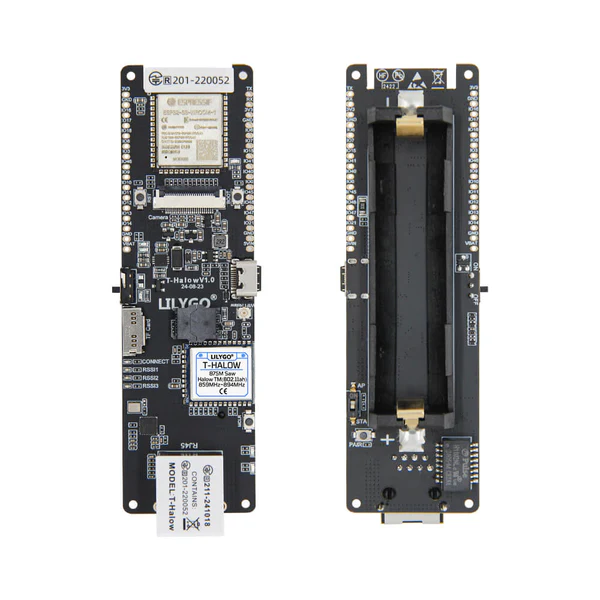
\includegraphics[width=1 \linewidth]{Documento/Imagenes/Análisis/Microcontroladores/lilygo-T-Halow.png}}
&
    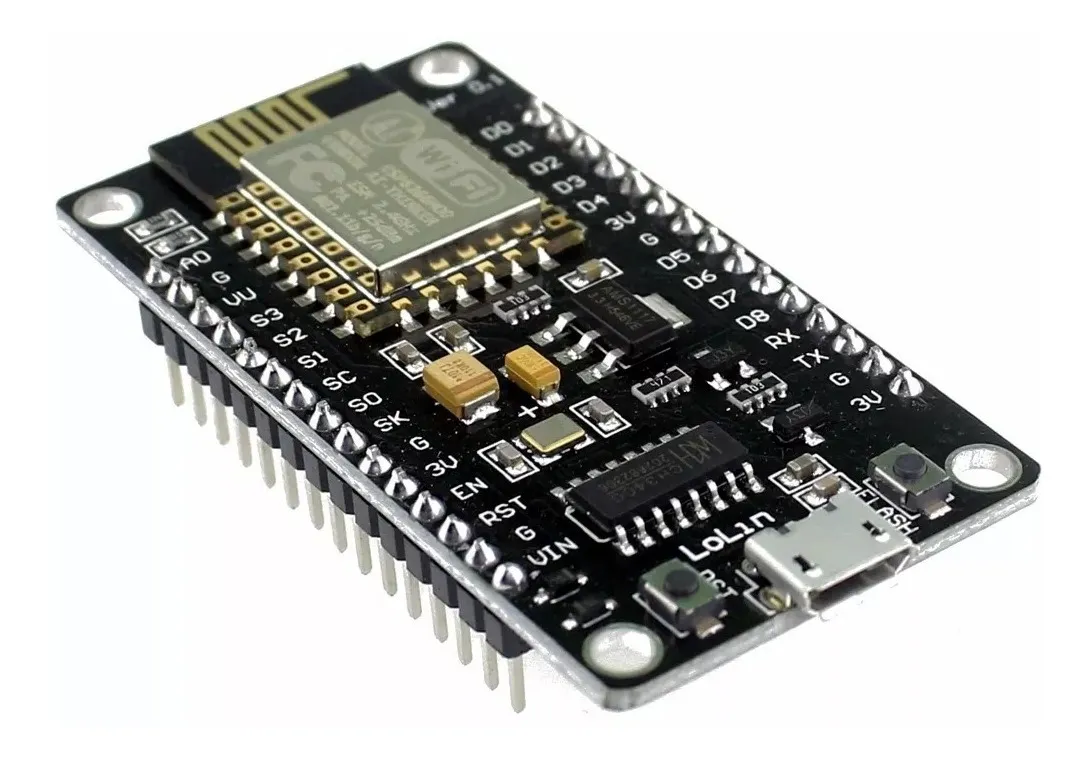
\includegraphics[width=1 \linewidth]{Documento/Imagenes/Análisis/Microcontroladores/NodeMCU.png}
&  
    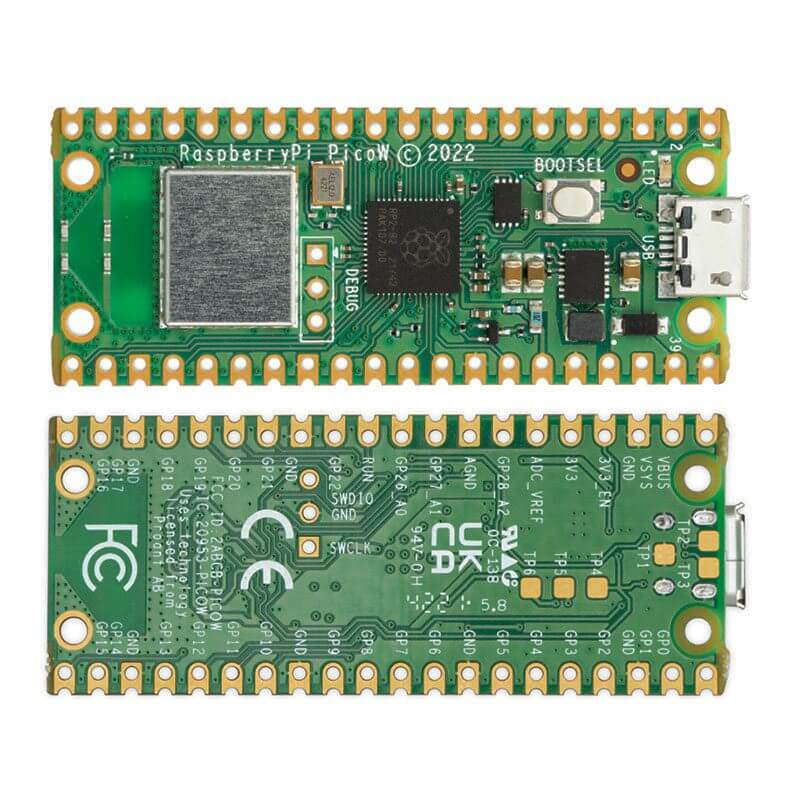
\includegraphics[width=0.9 \linewidth]{Documento/Imagenes/Análisis/Microcontroladores/RB Pico.jpg}   
\\ \hline

\end{longtable}




\begin{longtable}{|p{3cm}|p{4cm}|p{4cm}|p{4cm}|}
\hline
\multicolumn{4}{|c|}{Parte 2 Microcontroladores}\\
\hline
\textbf{Característica} 
& \textbf{Xiao ESP32-S3 R8} \cite{espressif2023_ESP32-S3}
& \textbf{STM32F103} \cite{stmicroelectronics2025_STM32F103ZE_datasheet}
& \textbf{ATmega328P} \cite{microchip2024_ATmega328P} \\
\hline
\endfirsthead

\hline
\textbf{Característica} 
& \textbf{Xiao ESP32-S3 R8} \cite{espressif2023_ESP32-S3}
& \textbf{STM32F103} \cite{stmicroelectronics2025_STM32F103ZE_datasheet}
& \textbf{ATmega328P} \cite{microchip2024_ATmega328P} \\
\hline
\endhead

\hline
\multicolumn{4}{r}{\textit{Continúa en la siguiente página}} \\
\endfoot

\hline
\endlastfoot

Arquitectura 
& Xtensa dual 32-bit LX7 
& ARM 32-bit M3 
& RISC 8-bit \\ \hline

Procesamiento 
& 240 MHz 
& 72 MHz 
& 16 MHz \\ \hline

RAM 
& 512KB + 8MB PSRAM 
& 64KB SRAM 
& 2KB SRAM \\ \hline

Flash 
& 8MB 
& 256–512KB 
& 32KB \\ \hline

Consumo Activo 
& 91 mA& 66 mA & 14 mA \\
Consumo Sleep & 240 \unit{\uA} & 8.5 mA & 60 \unit{\uA} \\ \hline

Voltaje & 3.3V & 5V & 5V \\ \hline

WiFi 
& 2.4GHz 
& No 
& No \\ \hline

Bluetooth 
& BLE 5 
& No 
& No \\ \hline

Sistema operativo (OS) 
& FreeRTOS 
& Bare-metal 
& Bare-metal \\ \hline

Costo (USD) 
& \$10–15 
& \$5 
& \$3 \\ \hline

Periféricos 
& \shortstack[l]{\\• 11 GPIOs\\• ADC (8 canales)\\• UART\\• SPI}
& \shortstack[l]{\\• 51 GPIOs\\• ADC (3 canales)\\• 5×UART\\• SPI}
& \shortstack[l]{\\• 23 GPIOs\\• ADC (8 canales)\\• USART\\• SPI} \\ \hline

Ventajas 
& \shortstack[l]{\\• RAM PSRAM (8MB)\\• Alto rendimiento\\• Bajo consumo \\• Compatible con \\tarjeta de expansión \\con cámara }
& \shortstack[l]{\\• Múltiples UARTs\\• Amplios GPIOs\\• Bajo costo}
& \shortstack[l]{\\• Amplia comunidad\\• Bajo consumo\\• Fácil prototipado} \\ \hline

Desventajas 
& \shortstack[l]{\\• GPIOs limitados\\• Costo moderado\\• Canales ADC\\ insuficientes}
& \shortstack[l]{\\• RAM limitada\\• Sin PSRAM\\• Procesamiento\\moderado}
& \shortstack[l]{\\• RAM mínima\\• Arquitectura 8-bit \\limitada} \\ \hline

Imagen 
& 
    \shortstack{\\ 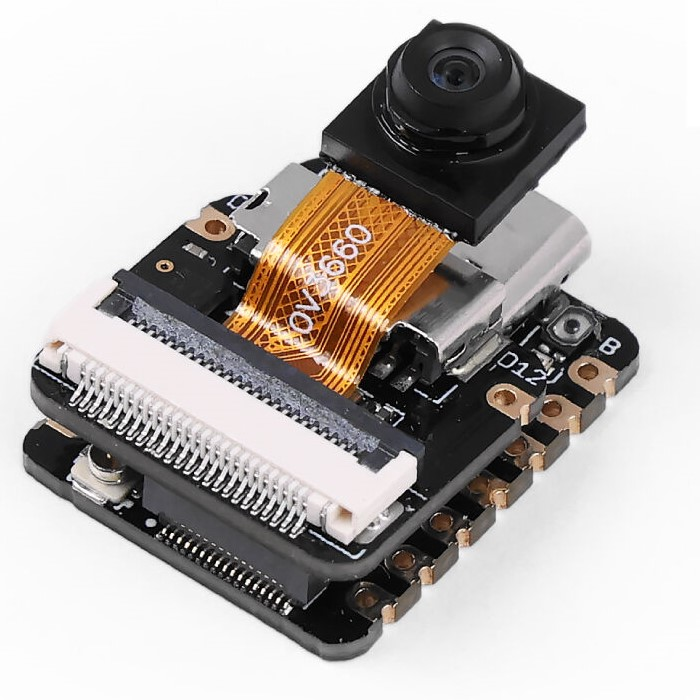
\includegraphics[width=1 \linewidth]{Documento/Imagenes/Análisis/Microcontroladores/xiao-esp32-s3-sense.jpg}}
&
    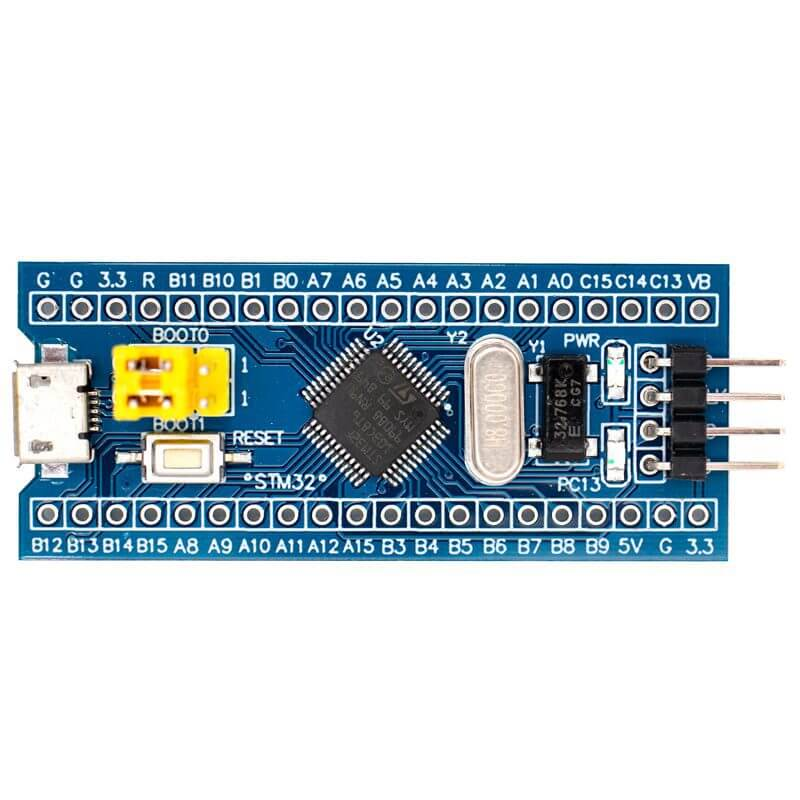
\includegraphics[width=1 \linewidth]{Documento/Imagenes/Análisis/Microcontroladores/STM32f103.jpg}
&  
    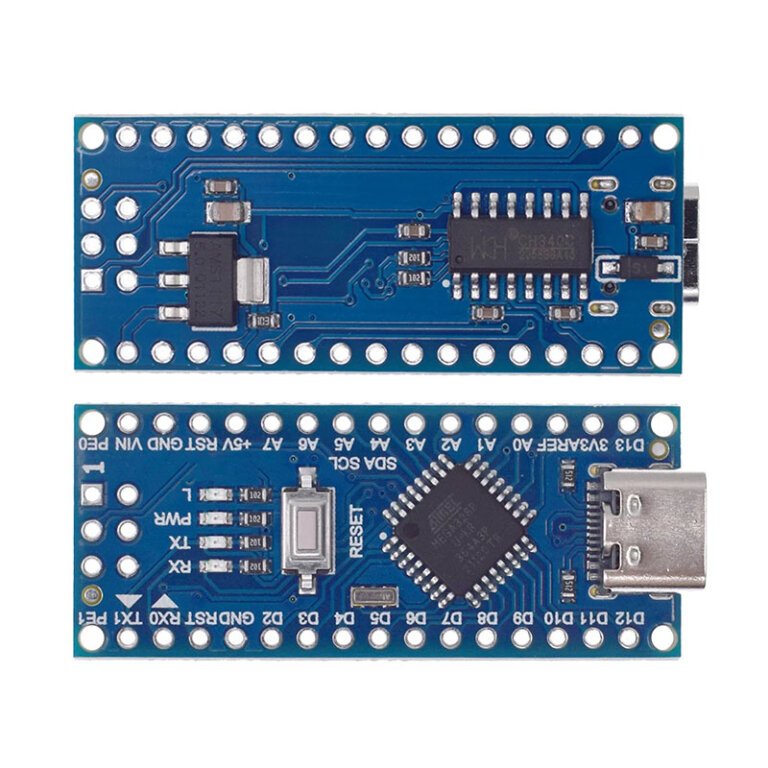
\includegraphics[width=0.9 \linewidth]{Documento/Imagenes/Análisis/Microcontroladores/Atmega328p.jpg}   
\\ \hline

\end{longtable}

\begin{longtable}{|p{3cm}|p{4cm}|p{4cm}|}
\hline
\multicolumn{3}{|c|}{Parte 3 Microcontroladores}\\
\hline
\textbf{Característica} 
& \textbf{Raspberry Pi Zero} \cite{raspberrypi_computers2025}
& \textbf{Raspberry Pi Zero 2 W} \cite{raspberrypi_computers2025}
 \\
\hline
\endfirsthead

\hline
\textbf{Característica} 
& \textbf{Raspberry Pi Zero} \cite{raspberrypi_computers2025}
& \textbf{Raspberry Pi Zero 2 W} \cite{raspberrypi_computers2025}
 \\
\hline
\endhead

\hline
\multicolumn{3}{r}{\textit{Continúa en la siguiente página}} \\
\endfoot

\hline
\endlastfoot

Arquitectura 
& ARM1176JZF-S 
& ARM Cortex-A53 (quad-core) 
 \\ \hline

Procesamiento 
& 1.0 GHz (single-core) 
& 1.0 GHz (quad-core) 
 \\ \hline

RAM 
& 512MB LPDDR2 
& 512MB LPDDR2 
 \\ \hline

Flash 
& microSD externa 
& microSD externa 
 \\ \hline

Consumo Activo 
&  2.5A
&  2.5A
 \\ \hline

Voltaje & 5V (microUSB) & 5V (microUSB)  \\ \hline

Broadcom chip & BCM2835 Single-core & RP3A0 Quad-core  \\ \hline

WiFi 
& Solo en modelo W: 2.4GHz (802.11n) 
& 2.4GHz (802.11n) 
 \\ \hline

Bluetooth 
& BLE 4.0 
& BLE 4.2 
 \\ \hline

Sistema operativo (OS) 
& Raspberry Pi OS (Linux) 
& Raspberry Pi OS (Linux) 
 \\ \hline

Costo (USD) 
& \$10 
& \$15 
 \\ \hline

Periféricos 
& \shortstack[l]{\\• 40 GPIOs\\• UART\\• SPI\\• I2C}
& \shortstack[l]{\\• 40 GPIOs\\• UART\\• SPI\\• I2C}
 \\ \hline

Ventajas 
& \shortstack[l]{\\• Bajo costo\\• Compatible con \\ecosistema Linux\\• Buena conectividad\\• Compacto}
& \shortstack[l]{\\• Multiprocesamiento \\(4 cores)\\• Más rápido que Zero\\• Ideal para visión\\ artificial}
 \\ \hline

Desventajas 
& \shortstack[l]{\\• Procesador antiguo\\• Capacidad de \\procesamiento limitada\\• Mayor consumo que \\MCUs}
& \shortstack[l]{\\• Sin GPIO analógicos\\• Requiere más energía \\que microcontroladores \\comunes}
 \\ \hline

Imagen 
& 
    \shortstack{\\ 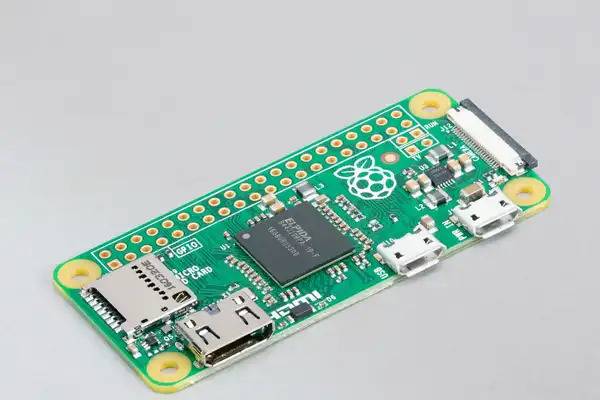
\includegraphics[width=0.9\linewidth]{Documento/Imagenes/Análisis/Microcontroladores/zerow.jpg}}
&
    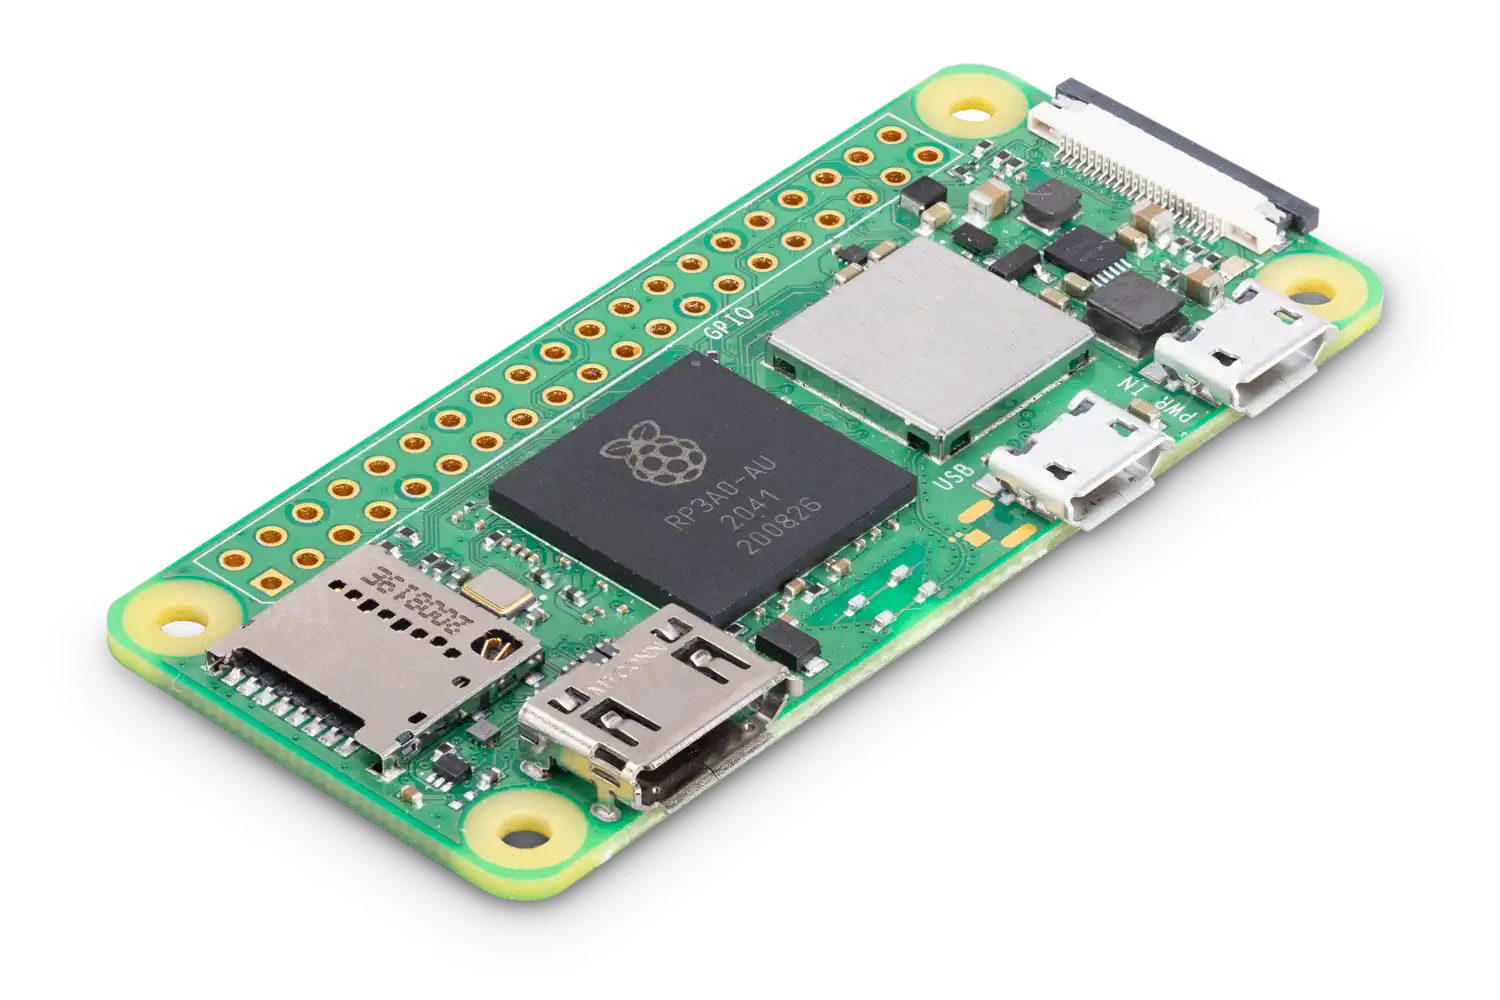
\includegraphics[width=0.9\linewidth]{Documento/Imagenes/Análisis/Microcontroladores/zero2w.jpg}

\\ \hline

\end{longtable}
 

\begin{table}[H]
\centering
\caption{Comparativa de microcontroladores para nodos fluviales}
\resizebox{\textwidth}{!}{
\begin{tabular}{|l|c|c|c|c|c|}
\hline
\textbf{MCU} & \textbf{Periféricos} & \textbf{Memoria} & \textbf{Consumo Activo} & \textbf{Consumo Sleep} & \textbf{Conectividad} \\ \hline
Xiao ESP32-S3 & 11 GPIOs, 8 ADC & 8MB Flash & 91 mA & 240 µA & WiFi 2.4GHz + BLE \\ \hline
LilyGO T-HaLow & 36 GPIOs, 20 ADC & 16MB Flash & 91 mA & 240 µA & WiFi HaLow (900MHz) \\ \hline
RPi Pico W & 23 GPIOs, 3 ADC & 2MB Flash & 50 mA & 390 µA & WiFi 2.4GHz \\ \hline
ESP8266 NodeMCU & 17 GPIOs, 1 ADC & 4MB Flash & 80 mA & 20 µA & WiFi 2.4GHz \\ \hline
RPi Zero W & 40 GPIOs (sin ADC) & Micro SD & 2.5 A & - & WiFi 2.4GHz + BLE 4.0 \\ \hline
RPi Zero 2 W & 40 GPIOs (sin ADC) & Micro SD & 2.5 A & - & WiFi 2.4GHz + BLE 4.2 \\ \hline
\end{tabular}
}
\end{table}

Para el nodo sensor y concentrador, encargado de capturar datos de sensores (pH, turbidez, oxígeno disuelto) y transmitir imágenes sin procesamiento, se considera preliminarmente la tarjeta Xiao ESP32-S3 debido a su interfaz completa con 8 canales ADC y puertos UART/SPI/I2C para conectar sensores y módulo HaLow, memoria suficiente de 8MB Flash para almacenamiento temporal de imágenes JPEG antes de transmisión, bajo consumo de 91mA en active mode y 10 µA en sleep mode ideal para operación con baterías, y costo competitivo de ~\$12 por unidad, cumpliendo con los requisitos de conectividad, eficiencia energética y manejo simultáneo de datos sensoriales e imágenes, aunque requiere validación experimental de estabilidad en transmisiones continuas y posibles limitaciones de GPIOs.

\subsection{Comparativa de microcontroladores PIC para control de sensores}
\label{subsec:comparativa_pic}

Dado que el Xiao ESP32-S3 Sense presenta un número limitado de pines GPIO disponibles (especialmente al estar asignados a la cámara OV5640 y al módulo Wi-Fi HaLow), se decidió incorporar un microcontrolador auxiliar dedicado exclusivamente a la gestión de sensores. Este microcontrolador debe ser de bajo consumo, tamaño reducido, fácil de programar y con recursos suficientes para:

\begin{itemize}
    \item Controlar encendido y apagado de sensores vía demultiplexor (74HC238).
    \item Leer señales analógicas mediante entradas ADC.
    \item Comunicarse con la Xiao ESP32.
    \item Mantener una operación eficiente en modo \textit{sleep}.
\end{itemize}

Con estos criterios, se evaluaron tres microcontroladores PIC de arquitectura de 8 bits con tecnología \textit{nanoWatt XLP}, comparados en la Tabla~\ref{tab:comparativa_pic}.

\begin{table}[H]
\centering
\caption{Comparativa de microcontroladores PIC para nodo sensor}
\label{tab:comparativa_pic}
\renewcommand{\arraystretch}{1.4}
\begin{tabular}{@{}|l|c|c|c|@{}}
\hline
\textbf{Característica} & \textbf{PIC12LF1822} \cite{microchip2020_PIC12LF1822_16LF1823}
                        & \textbf{PIC16LF1823} \cite{microchip2020_PIC12LF1822_16LF1823}
                        & \textbf{PIC16LF1847} \cite{microchip2013_PIC16LF1847}\\
\hline
Arquitectura         & 8-bit & 8-bit & 8-bit \\ \hline
GPIO disponibles     & 6     & 12    & 16 \\ \hline
Entradas ADC         & 4     & 8     & 12 \\ \hline
Módulo UART (EUSART) & Sí    & Sí    & Sí \\ \hline
Módulo SPI & Sí    & Sí    & Sí \\ \hline
Módulo I2C & Sí    & Sí    & Sí \\ \hline
Frecuencia máx. (MHz)& 32    & 32    & 32 \\ \hline
Consumo \textit{Sleep} & 20 nA & 20 nA & 20 nA \\ \hline
Consumo activo (@1MHz) & 30~\unit{uA} & 30~\unit{uA} & 65~\unit{uA} \\ \hline
Memoria Flash (Bytes) & 2048  & 2048  & 8192 \\ \hline
RAM (Bytes)           & 128   & 128   & 1024 \\ \hline
Tamaño encapsulado    & 8 pines & 14 pines & 28 pines \\ \hline
Precio aproximado (USD) & \$3 & \$3 & \$3 \\ \hline
\end{tabular}
\end{table}


El modelo seleccionado para el diseño del nodo es el \textbf{PIC16LF1823}, ya que representa el punto óptimo entre capacidad, eficiencia y costo:

\begin{itemize}
    \item Dispone de 11 pines GPIO, suficientes para controlar el DEMUX (3 líneas), adquirir hasta 8 señales analógicas y mantener UART dedicado.
    \item Integra un módulo EUSART que permite comunicación estable con el Xiao ESP32.
    \item Su bajo consumo en modo \textit{sleep} (20nA) y modo activo (50\unit{uA}/MHz) lo hacen ideal para sistemas alimentados por batería.
    \item Su encapsulado de 14 pines facilita el montaje en placas compactas sin sacrificar funcionalidad.
    \item Presenta compatibilidad con herramientas estándar de Microchip (MPLAB X, XC8).
\end{itemize}

En contraste, el PIC12LF1822 resulta limitado en pines y entradas ADC, mientras que el PIC16LF1847 ofrece mayores recursos a costa de un tamaño físico mayor, mayor consumo y un costo menos competitivo, innecesario para esta aplicación específica.



%%%%%%%%%%%%%%%%%%%%%%%%%%%%%%%%%%%%%%%%%%%%%%%%%%%%
%             SECCIÓN: Alimentación                %
%%%%%%%%%%%%%%%%%%%%%%%%%%%%%%%%%%%%%%%%%%%%%%%%%%%%


\section{Análisis de la Alimentación}
\label{sec:analisis_alimentacion}

El sistema de monitoreo propuesto está diseñado para operar de forma autónoma en entornos naturales remotos, donde no se dispone de infraestructura eléctrica. Por ello, el subsistema de alimentación eléctrica representa un componente crítico para garantizar la continuidad operativa. La solución adoptada se basa en el uso de baterías recargables de ion-litio, complementadas con paneles solares y un módulo de gestión de carga, asegurando la autosuficiencia energética de los nodos sensores distribuidos.

\subsection{Requerimientos de Alimentación de los Componentes}
\label{subsec:reqs_alimentacion}

La Tabla~\ref{tab:componentes_energia} presenta los principales componentes seleccionados para el nodo sensor (ver secciones \ref{sec:analisis_microcontroladores} y \ref{sec:analisis_sensores}), junto con sus requerimientos estimados de voltaje y corriente de operación, extraídos de sus respectivas hojas de datos. Estos valores son fundamentales para dimensionar el sistema de alimentación.

%\renewcommand{\arraystretch}{1.4}
\begin{longtable}{|p{5cm}|c|c|}
\caption{Consumo eléctrico de componentes}
\label{tab:componentes_energia} \\
\hline
\textbf{Componente} & \textbf{Voltaje} & \textbf{Corriente} \\
\hline
\endfirsthead

\hline
\textbf{Componente} & \textbf{Voltaje} & \textbf{Corriente} \\
\hline
\endhead

\hline
\multicolumn{3}{r}{\textit{Continúa en la siguiente página}} \\
\endfoot

\hline
\endlastfoot

\multicolumn{3}{|c|}{\textbf{Transceptor}} \\
\hline
\multirow{6}{*}{Quectel FGH100MHAAMD}& \multirow{6}{*}{3.3V} & \textbf{Modo Tx}\\
     &  & 54 \unit{\mA} \\ \cline{3-3}
     &  & \textbf{Modo RX} \\
     &  & 43 \unit{\mA} \\ \cline{3-3}
     &  & \textbf{Modo Sleep} \\
     &  & $<10$ \unit{\uA} \\
\hline

\multicolumn{3}{|c|}{\textbf{Microcontrolador}} \\
\hline
\multirow{4}{*}{ESP32-S3R8} & \multirow{4}{*}{3.3V} & \textbf{Modo activo} \\
   &  & 91 \unit{\mA} \\ \cline{3-3}
   &  & \textbf{Modo Sleep} \\
   &  & 240 \unit{\uA} \\
\hline

\multicolumn{3}{|c|}{\textbf{Sensores}} \\
\hline
Sensor de pH (Gravity V2)                & 5V         & 10 \unit{\mA} \\
Sensor de oxígeno disuelto               & 5V         & 10–50 \unit{\mA} \\
Sensor de turbidez                       & 5V         & 20–30 \unit{\mA} \\
Sensor de conductividad eléctrica        & 5V         & 30–40 \unit{\mA} \\
Sensor de temperatura (DS18B20)          & 3.3 - 5V   & 4 \unit{\mA} \\
\hline

\multicolumn{3}{|c|}{\textbf{Cámara}} \\
\hline
\multirow{4}{*}{Cámara OV2640}           & \multirow{4}{*}{3.3 - 5V} & \textbf{Active}  \\
& & 140 \unit{\mA}\\
                                         &                           & \textbf{Standby}  \\
& & 20 \unit{\uA} \\                                        
\hline
\end{longtable}





\begin{table}[H]
\centering
\caption{Consumo eléctrico estimado de componentes del nodo sensor.}
\label{tab:componentes_energia}
\renewcommand{\arraystretch}{1.2}
\begin{tabular}{l l S[table-format=1.1] S[table-format=3.3] l}
\toprule
\textbf{Componente} & \textbf{Modo} & {\textbf{Voltaje}} & {\textbf{Corriente}} & \textbf{Ref.} \\
 & & {(\unit{\volt})} & {(\unit{\milli\ampere})} & \\
\midrule
\multirow{3}{*}{Transceptor FGH100M} & Tx & 3.3 & 54 & \cite{QuectelFGH100M} \\ 
 & Rx & 3.3 & 43 & \cite{QuectelFGH100M} \\
 & Sleep & 3.3 & <0.010 & \cite{QuectelFGH100M} \\
\midrule
\multirow{2}{*}{MCU Xiao ESP32-S3} & Activo & 3.3 & 91 & \cite{espressif2023_ESP32-S3} \\ 
 & Sleep & 3.3 & 0.240 & \cite{espressif2023_ESP32-S3} \\
\midrule
MCU PIC16LF1823 & Activo (@ \SI{1}{\mega\hertz}) & 3.3 & 0.050 & \cite{microchip2020_PIC12LF1822_16LF1823} \\ 
 & Sleep & 3.3 & <0.001 & \cite{microchip2020_PIC12LF1822_16LF1823} \\
\midrule
Sensor pH (Industrial V2) & Activo & 5.0 & 10 & \cite{DFRobot_pH_Sensor} \\ 
Sensor OD (SEN0237) & Activo & 5.0 & 40 & \cite{DFRobot_DO_Sensor} \\
Sensor Turbidez (SEN0189) & Activo & 5.0 & 30 & \cite{DFRobot_Turbidity_Sensor} \\ 
Sensor EC (DFR0300) & Activo & 5.0 & 40 & \cite{DFRobot_EC_Sensor} \\
Sensor Temp (DS18B20) & Activo & 3.3 & 4 & \cite{DFRobot_DS18B20} \\ 
\midrule
\multirow{2}{*}{Cámara OV5640} & Activo & 3.3 & 140 & \cite{omnivision2011_OV5640} \\ 
 & Standby & 3.3 & 0.020 & \cite{omnivision2011_OV5640} \\
\bottomrule
\end{tabular}
\end{table}
 


Para estimar de forma realista el consumo energético del sistema, es indispensable cuantificar la duración efectiva de las fases de transmisión y recepción de datos, considerando el volumen de información y la velocidad de comunicación del transceptor Wi-Fi HaLow (FGH100M).


\subsubsection{Volumen de Datos a Transmitir por Ciclo}
\label{ssubsec:volumen_datos}
Cada nodo sensor genera dos tipos de información por ciclo operativo semanal:

\begin{enumerate}
    \item \textbf{Una muestra sensorial única}, compuesta por:
    \begin{itemize}
        \item 4 sensores analógicos (asumiendo ADC de 12 bits): 
        $4 \times \SI{12}{\bit} = \SI{48}{\bit} = \SI{6}{\byte}$
        \item 1 sensor digital (DS18B20, resolución \SI{12}{\bit}): \SI{2}{\byte}
        \item Metadatos (Timestamp + ID de nodo + tipo de trama, estimado): \SI{8}{\byte}
    \end{itemize}
    \[
    \text{Volumen}_{\text{sensores}} = 6 + 2 + 8 = \boxed{\SI{16}{\byte}}
    \]

    \item \textbf{Una única imagen} capturada por la cámara (ej. OV5640). 
    Se asume una resolución de \(640 \times 480\) píxeles y una compresión JPEG que resulta en un tamaño de archivo típico de \SI{150}{\kilo\byte} \cite{jpegCompression}. 
    Esta compresión es crucial para reducir el volumen de datos a transmitir.
    \[
    \text{Volumen}_{\text{imagen}} = \SI{150}{\kilo\byte} = \num{153600}\,\text{bytes}
    \]
\end{enumerate}

El volumen total de datos generado por un nodo en cada ciclo es la suma de ambos:
\[
\text{Volumen}_{\text{nodo}} = \text{Volumen}_{\text{sensores}} + \text{Volumen}_{\text{imagen}} \approx \SI{153616}{bytes} \approx \SI{150.02}{\kilo\byte}
\]

\subsubsection{Tiempo Estimado de Transmisión}
\label{ssubsec:tiempo_tx}
Se asume una tasa de transmisión efectiva (\textit{throughput}) para el enlace Wi-Fi HaLow (FGH100M) de \SI{1}{\mega\bit\per\second}. Esta es una estimación conservadora, considerablemente menor que la tasa teórica máxima (ej. \SI{4.4}{\mega\bit\per\second} con MCS 7 @ \SI{8}{\mega\hertz}), para tener en cuenta el overhead del protocolo (cabeceras, ACK), posibles retransmisiones y las condiciones del canal en un entorno real \cite{ieee80211ah}.

Bajo esta condición:
\[
T_{\text{transmisión-nodo}} = \frac{\text{Volumen}_{\text{nodo}} \times 8\,\text{bits/byte}}{\text{Tasa de transmisión}} = \frac{\num{153616} \times 8}{\SI{1e6}{\bit\per\second}} \approx \num{1.229}\,\unit{\second}
\]
Por lo tanto, el tiempo activo estimado para transmitir los datos de un nodo es de aproximadamente \textbf{\SI{1.23}{\second}}.


\subsubsection{Tiempo Total de Comunicación por Nodo en Topología Lineal}
\label{ssubsec:tiempo_general_comm}

El protocolo IEEE 802.11ah opera en modo \textit{half-duplex}, impidiendo la transmisión y recepción simultáneas \cite{ieee80211ah}. En la topología lineal adoptada, esto tiene un impacto acumulativo en el tiempo de actividad de cada nodo.

Consideremos una red lineal con $N$ nodos sensores (numerados del 1 al $N$), donde el Nodo 1 es el más alejado del concentrador y el Nodo $N$ es el más cercano. El concentrador se considera como el destino final después del Nodo $N$.

El tiempo base ($T_{base}$) para transmitir el volumen de datos ($V_n$) generado por un solo nodo en cada ciclo se calcula como:
\begin{equation} \label{eq:tiempo_base}
T_{base} = \frac{V_n \times 8}{R}
\end{equation}
Donde:
\begin{itemize}
    \item $T_{base}$ es el tiempo base de transmisión por nodo (en segundos).
    \item $V_n$ es el volumen de datos generado por un nodo por ciclo (en bytes).
    \item $R$ es la tasa de transmisión efectiva del enlace (en bits por segundo).
    \item 8 es el factor de conversión de bytes a bits.
\end{itemize}

Un nodo genérico $n$ (donde $1 \le n \le N$) debe recibir los datos de los $n-1$ nodos anteriores y transmitir los $n$ paquetes acumulados (los $n-1$ recibidos más el suyo). Los tiempos de recepción ($T_{rx}$) y transmisión ($T_{tx}$) para el nodo $n$ son:
\begin{equation} \label{eq:tiempo_rx_n}
T_{rx}(n) = (n-1) \times T_{base}
\end{equation}
\begin{equation} \label{eq:tiempo_tx_n}
T_{tx}(n) = n \times T_{base}
\end{equation}
Donde:
\begin{itemize}
    \item $T_{rx}(n)$ es el tiempo total de recepción para el nodo $n$ (en segundos).
    \item $T_{tx}(n)$ es el tiempo total de transmisión para el nodo $n$ (en segundos).
    \item $n$ es el índice del nodo en la cadena lineal (1 a N).
    \item $T_{base}$ es el tiempo base de transmisión por nodo (calculado en \eqref{eq:tiempo_base}).
\end{itemize}

Por lo tanto, la fórmula general para el tiempo total de comunicación activa ($T_{comm}$) para un nodo $n$ en la cadena lineal es la suma de sus tiempos de recepción y transmisión:
\begin{equation} \label{eq:tiempo_comm_nodo_n}
T_{comm}(n) = T_{rx}(n) + T_{tx}(n) = ((n-1) + n) \times T_{base} = (2n - 1) \times T_{base}
\end{equation}
Donde:
\begin{itemize}
    \item $T_{comm}(n)$ es el tiempo total de comunicación activa para el nodo $n$ (en segundos).
    \item $n$ es el índice del nodo en la cadena lineal (1 a N).
    \item $T_{base}$ es el tiempo base de transmisión por nodo (calculado en \eqref{eq:tiempo_base}).
\end{itemize}

\paragraph{Ejemplo de Cálculo para el Nodo 4 (N=4):}
En este proyecto, se tienen $N=4$ nodos sensores. El nodo más cargado es el Nodo 4. Aplicando la Ecuación \eqref{eq:tiempo_comm_nodo_n} con $n=4$ y utilizando $T_{base} \approx \SI{1.23}{\second}$ (calculado en la subsección \ref{ssubsec:tiempo_tx} usando la Ecuación \eqref{eq:tiempo_base}):

\[
T_{comm}(4) = (2 \times 4 - 1) \times \SI{1.23}{\second} = 7 \times \SI{1.23}{\second} = \boxed{\SI{8.61}{\second}}
\]

Este valor representa el tiempo total que el Nodo 4 pasa en modos activos de comunicación por ciclo y será utilizado para el cálculo del consumo energético.


\subsection{Escenario Operativo}
\label{subsec:escenario_operativo}

Para optimizar el consumo energético y garantizar una larga autonomía, el sistema opera en un ciclo de bajo ciclo de trabajo (\textit{low duty cycle}). Se establece un **ciclo operativo semanal** (\SI{168}{\hour}) como referencia. Esta frecuencia se considera adecuada para el monitoreo ambiental de cuerpos de agua lóticos, permitiendo detectar tendencias a mediano plazo sin incurrir en un consumo excesivo \cite{nom001}.

Dentro de cada ciclo semanal, el nodo alterna entre modos de bajo consumo (\textit{sleep}) y modos activos para la adquisición y transmisión de datos. Considerando el nodo con mayor carga (Nodo 4), el tiempo estimado en cada modo por ciclo es el siguiente (ver Figura \ref{fig:ciclo_mod_op}):

\begin{itemize}
    \item \textbf{Adquisición de Datos}:
        \begin{itemize}
            \item Lectura de Sensores: Se asume un tiempo de estabilización y lectura de \SI{5}{\second} por cada uno de los 5 sensores, activados secuencialmente. Tiempo total = $5 \times \SI{5}{\second} = \SI{25}{\second}$.
            \item Captura de Imagen: Se estima un tiempo de \SI{10}{\second} para activar la cámara, capturar una imagen y almacenarla en el búfer. % Justificación: Tiempo típico estimado
        \end{itemize}
        Tiempo total de adquisición $\approx \SI{35}{\second}$.
    \item \textbf{Comunicación (Nodo 4)}: Tiempo total de Tx y Rx calculado previamente (ver \ref{ssubsec:tiempo_general_comm}) $\approx \SI{8.61}{\second}$.
    \item \textbf{Procesamiento Local (Estimado)}: Tiempo adicional para que el microcontrolador organice datos, comprima imagen (si aplica), etc. Se estima un tiempo conservador de \SI{5}{\second}. % Justificación: Estimación conservadora
    \item \textbf{Tiempo Activo Total por Ciclo}: $35 + 8.61 + 5 = \SI{48.61}{\second} \approx \SI{0.81}{\minute}$.
    \item \textbf{Tiempo en Modo Sleep}: $\SI{168}{\hour} - \SI{48.61}{\second} \approx \SI{167.987}{\hour}$ (aproximadamente el \SI{99.99}{\percent} del ciclo).
\end{itemize}

\begin{figure}[H]
    \centering
    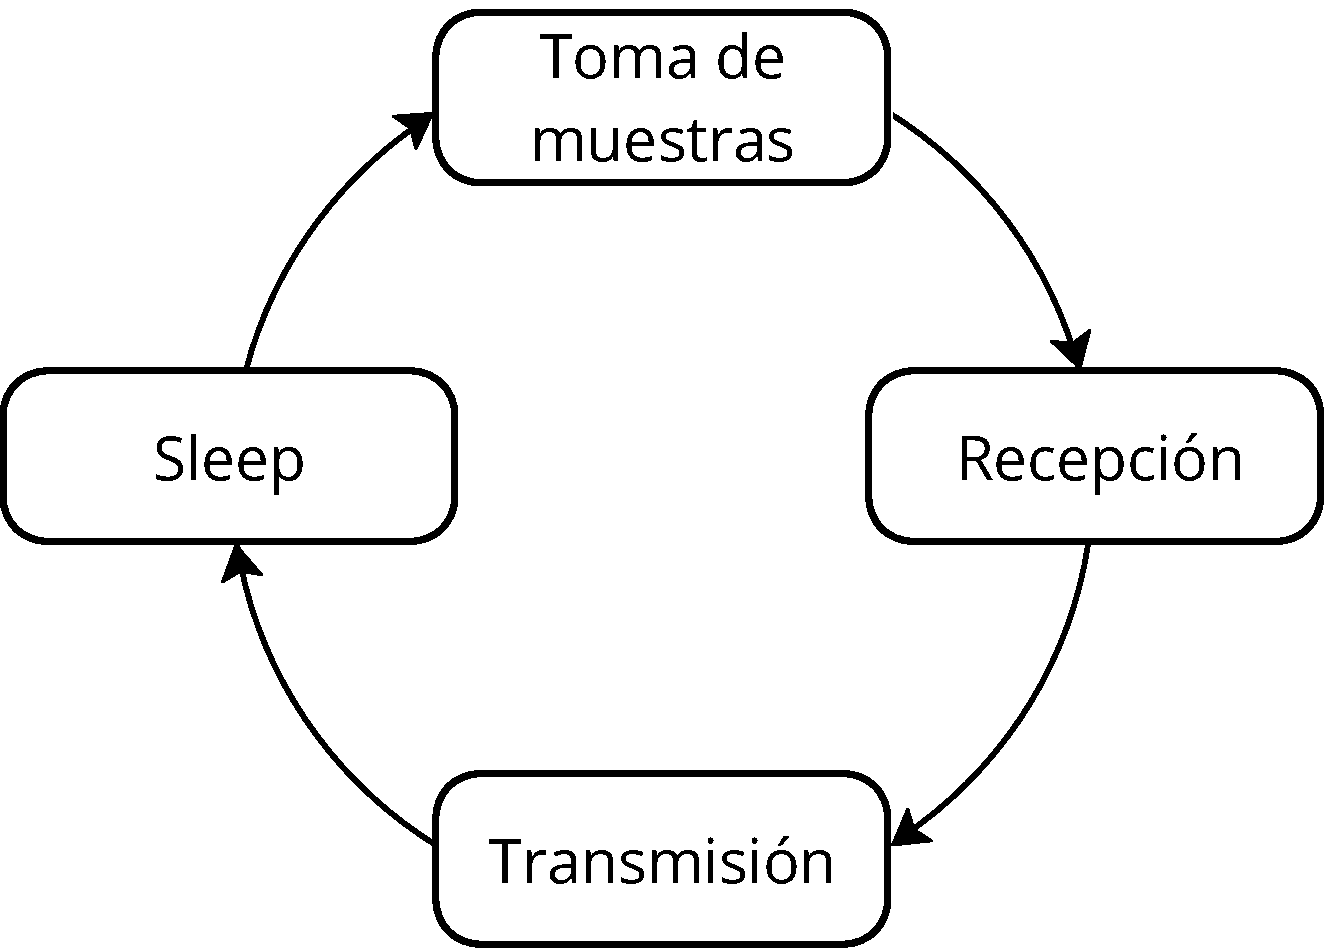
\includegraphics[width=0.5\linewidth]{Documento/Imagenes/Análisis/ciclo modos op.pdf} % Revisa el nombre del archivo si es necesario
    \caption{Ciclo simplificado de modos operativos del nodo sensor.}
    \label{fig:ciclo_mod_op}
\end{figure}




\subsection{Cálculo del Consumo Energético Semanal}
\label{subsec:calculo_consumo}

Utilizando los tiempos de operación estimados para cada modo y las corrientes de consumo de la Tabla \ref{tab:componentes_energia}, se calcula el consumo energético total por ciclo semanal ($E_{\text{sem}}$) para el nodo más demandante (Nodo 4). La fórmula general es:

\begin{equation} \label{eq:energia_semanal}
E_{\text{sem}} = \sum_{\text{modo}} (I_{\text{modo}} \times t_{\text{modo}})
\end{equation}

Para la fase de comunicación del Nodo 4, se separan los tiempos y corrientes de recepción (Rx) y transmisión (Tx) calculados en la subsección \ref{ssubsec:tiempo_general_comm}:
\begin{itemize}
    \item Tiempo de Recepción ($T_{rx}(4)$) = \SI{3.69}{\second}
    \item Tiempo de Transmisión ($T_{tx}(4)$) = \SI{4.92}{\second}
\end{itemize}
Las corrientes totales durante estas fases son:
\begin{itemize}
    \item Corriente en Rx ($I_{Rx}$) = $I_{\text{ESP32\_activo}} + I_{\text{FGH100M\_Rx}} = \SI{91}{\milli\ampere} + \SI{43}{\milli\ampere} = \SI{134}{\milli\ampere}$
    \item Corriente en Tx ($I_{Tx}$) = $I_{\text{ESP32\_activo}} + I_{\text{FGH100M\_Tx}} = \SI{91}{\milli\ampere} + \SI{54}{\milli\ampere} = \SI{145}{\milli\ampere}$
\end{itemize}

La Tabla \ref{tab:consumo_detallado_semanal} detalla el cálculo completo.

\begin{table}[H] 
\centering
\caption{Cálculo detallado del consumo energético semanal estimado (Nodo 4) con Tx/Rx separados.}
\label{tab:consumo_detallado_semanal}
\renewcommand{\arraystretch}{1.3}
\sisetup{round-mode=places, round-precision=2} % Redondeo a 2 decimales para la energía
\begin{tabular}{l S[table-format=3.3] S[table-format=6.3] S[table-format=3.2]}
\toprule
\textbf{Modo Operativo} & {\textbf{Corriente Total}} & {\textbf{Tiempo}} & {\textbf{Energía}} \\
 & {(\unit{\milli\ampere})} & {(\unit{\hour})} & {(\unit{\milli\ampere\hour})} \\
\midrule
Lectura Sensores (PIC + ESP32 + 1 Sensor) & 141.05 & {$25/3600$} & {$\approx \num{0.98}$} \\
Captura Imagen (ESP32 + Cam) & 231.24 & {$10/3600$} & {$\approx \num{0.64}$} \\
Recepción (Rx) (ESP32 + FGH Rx) & 134.00 & {$3.69/3600$} & {$\approx \num{0.14}$} \\ % Separado Rx
Transmisión (Tx) (ESP32 + FGH Tx) & 145.00 & {$4.92/3600$} & {$\approx \num{0.20}$} \\ % Separado Tx
Procesamiento Local (ESP32 + PIC) & 91.05 & {$5/3600$} & {$\approx \num{0.13}$} \\
Modo Sleep (Todo en sleep/standby) & 0.271 & 167.987 & {$\approx \num{45.52}$} \\
\midrule
\textbf{Total Estimado} & & & {$\approx \num{47.61}$} \\ % Nueva suma redondeada
\bottomrule
\end{tabular}
\end{table}
%\sisetup{round-mode=off} % Desactivar redondeo global si no se necesita más

El consumo energético total estimado por nodo por semana es de aproximadamente \textbf{\SI{47.6}{\milli\ampere\hour}}. Este valor se utilizará para dimensionar los componentes del subsistema de alimentación.

\subsection{Análisis y Selección de Componentes de Alimentación}
\label{subsec:seleccion_hardware_alimentacion}

Basándose en el consumo energético semanal estimado de \SI{47.6}{\milli\ampere\hour}, se procede a seleccionar los componentes del subsistema de alimentación: batería, panel solar y módulo de carga, buscando un balance entre capacidad, eficiencia, costo y seguridad.


\subsubsection{Análisis y Selección de la Batería}
La elección de la batería recargable es crucial para la autonomía del nodo. Se compararon opciones Li-ion y LiPo disponibles comercialmente (Tabla \ref{tab:baterias}), considerando capacidad, ciclos de vida, seguridad (presencia de BMS) y dimensiones.

% --- Tabla Comparativa Baterías ---
\renewcommand{\arraystretch}{1.5}
\begin{longtable}{|p{4.2cm}|c|c|c|}
\caption{Comparativa de baterías recargables para el nodo sensor}
\label{tab:baterias} \\
\hline
\textbf{Característica} & \textbf{104050} \cite{batteryLipo104050}
                        & \textbf{18650 2200mAh} \cite{batteryLiIon18650}
                        & \textbf{18650 3000mAh} \cite{batteryLiIon18650} \\
\hline
\endfirsthead

\hline
\textbf{Característica} & \textbf{104050} \cite{batteryLipo104050}
                        & \textbf{18650 2200mAh} \cite{batteryLiIon18650}
                        & \textbf{18650 3000mAh} \cite{batteryLiIon18650} \\
\hline
\endhead

\hline
\multicolumn{4}{r}{\textit{Continúa en la siguiente página}} \\
\endfoot

\hline
\endlastfoot

Tipo de batería & LiPo & Li-ion & Li-ion \\
\hline
Capacidad (mAh) & 2500 & 2200 & 3000 \\
\hline
Voltaje nominal (V) & 3.7 & 3.7 & 3.7 \\
\hline
Corriente máxima de descarga (A) & 2.5 & 2.2 & 3 \\
\hline
Dimensiones (mm) & 50x40x10 & 18x65 & 18x65 \\
\hline
Peso (g) & 44 & 43 & 46 \\
\hline
Número de ciclos de carga & $>800$ & $>1000$ & $>1000$ \\
\hline
Protección integrada (BMS) & Sí & No & No \\
\hline
Precio aproximado (MXN) & \$150 & \$80 & \$100 \\
\hline
Imagen 
& \shortstack{\\ 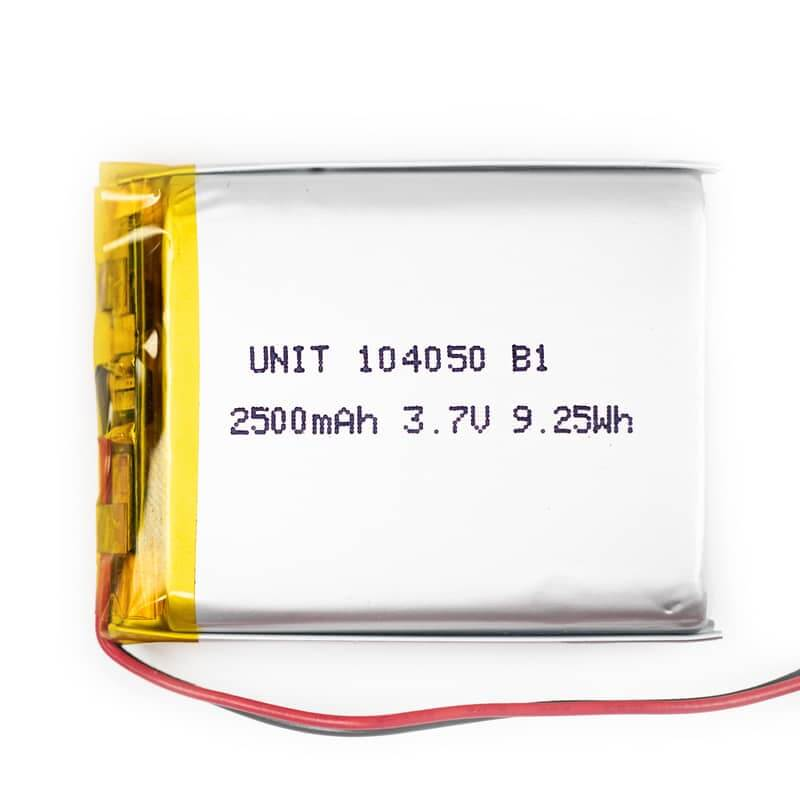
\includegraphics[scale=0.1]{Documento/Imagenes/Análisis/Bat-Pan/Bateria-104050.jpg}}
& \shortstack{\\ 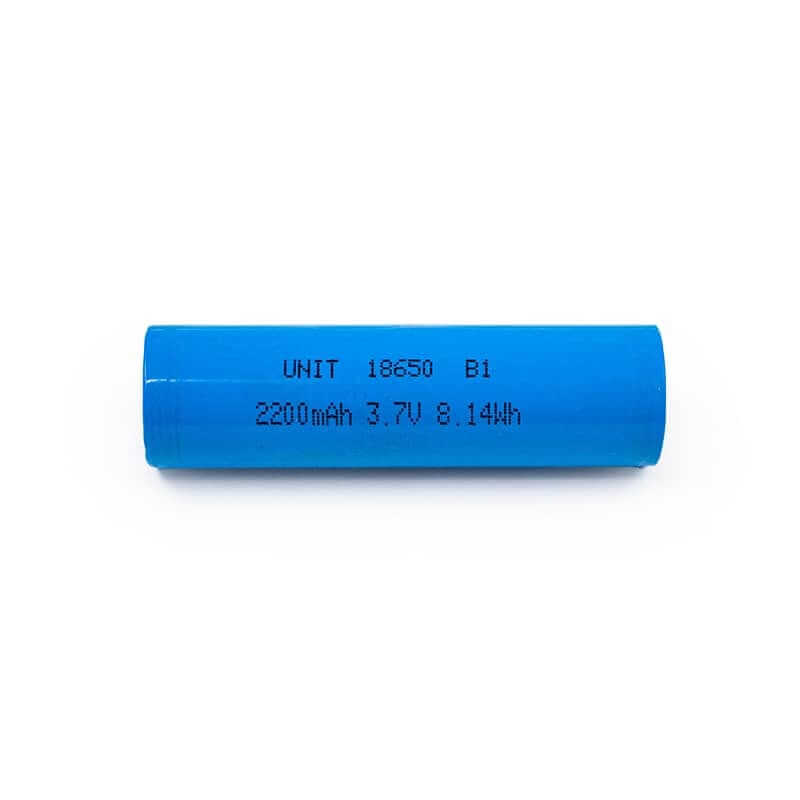
\includegraphics[scale=0.11]{Documento/Imagenes/Análisis/Bat-Pan/Bateria-18650-2200mAh.jpg}}
& \shortstack{\\ 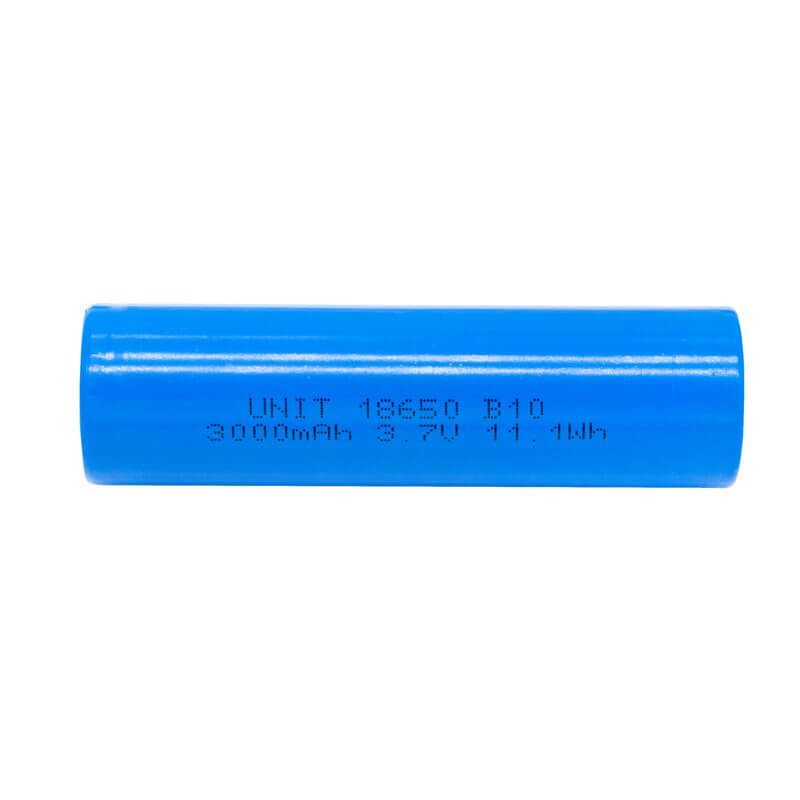
\includegraphics[scale=0.1]{Documento/Imagenes/Análisis/Bat-Pan/Bateria-18650-3000mAh.jpg}} \\
\end{longtable}


 Se selecciona la batería \textbf{LiPo modelo 104050} con una capacidad nominal de \SI{2500}{\milli\ampere\hour}. Aunque las celdas Li-ion 18650 ofrecen un mayor número de ciclos de vida teóricos, la LiPo seleccionada presenta dos ventajas clave para este proyecto:
\begin{enumerate}
    \item \textbf{Seguridad Integrada:} Incluye un circuito de protección (BMS - Battery Management System) incorporado, que previene sobrecargas, sobredescargas y cortocircuitos, crucial para un dispositivo autónomo desatendido \cite{batteryLipo104050}.
    \item \textbf{Capacidad Suficiente:} Sus \SI{2500}{\milli\ampere\hour} exceden ampliamente la demanda energética calculada, proporcionando un gran margen de seguridad.
\end{enumerate}
La opción Li-ion 18650 requeriría un BMS externo, añadiendo complejidad al diseño.

\paragraph{Cálculo de Autonomía Teórica:} Con la batería seleccionada, la autonomía estimada sin recarga solar es:
\begin{equation} \label{eq:autonomia}
\text{Autonomía} = \frac{\text{Capacidad Batería}}{\text{Consumo Semanal}} = \frac{\SI{2500}{\milli\ampere\hour}}{\SI{47.6}{\milli\ampere\hour / \text{sem}}} \approx \boxed{\num{52.5}~\text{semanas}} \approx \num{367}~\text{días}
\end{equation}
Este cálculo sugiere una autonomía teórica de casi un año, ofreciendo una excelente resiliencia ante periodos prolongados sin sol.

\subsubsection{Análisis y Selección del Panel Solar}
Para garantizar la operación continua, se necesita un panel solar que reponga el consumo energético. Se evaluaron paneles compactos (Tabla \ref{tab:paneles_solares}) en función de su potencia, voltaje/corriente de salida y dimensiones.

\begin{table}[H]
\centering
\renewcommand{\arraystretch}{1.5}
\caption{Comparativa de paneles solares para el nodo sensor}
\label{tab:paneles_solares}
\begin{tabular}{|p{4cm}|c|c|c|}
\hline
\textbf{Característica} & \textbf{Panel 5V} \cite{panelSolar5V}
                        & \textbf{Panel 6V} \cite{panelSolar6V}
                        & \textbf{Panel 12V} \cite{panelSolar12V} \\
\hline
Potencia nominal (W) & 1.9 & 1.92 & 3 \\\hline
Corriente de salida (mA) & 320 & 320 & 250 \\
\hline
Voltaje de salida (V) & 5 & 6 & 12 \\
\hline
Medición de intensidad de luz & \multicolumn{3}{|c|}{38000 LUX} \\
\hline
Dimensiones (mm) & 135x130 & 104x140 & 145x145 \\
\hline
Peso (g) & 65 & 54 & 34 \\
\hline
Precio aproximado (USD) & \$6 & \$5 & \$7 \\
\hline
Imagen 
&\shortstack{\\ 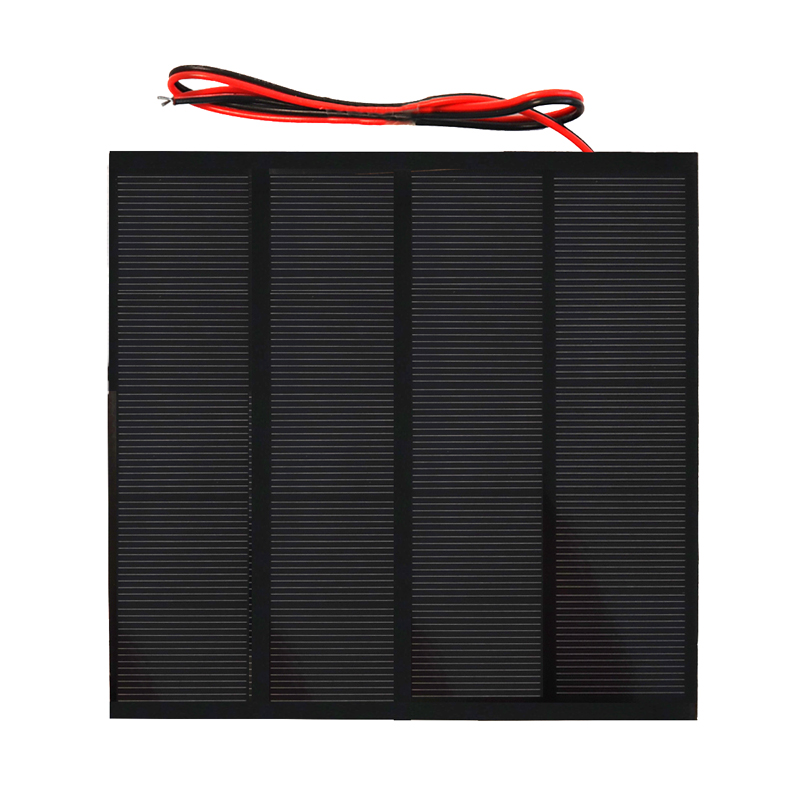
\includegraphics[scale = 0.1]{Documento/Imagenes/Análisis/Bat-Pan/PanelSolar-5V.jpg}}
& \shortstack{\\ 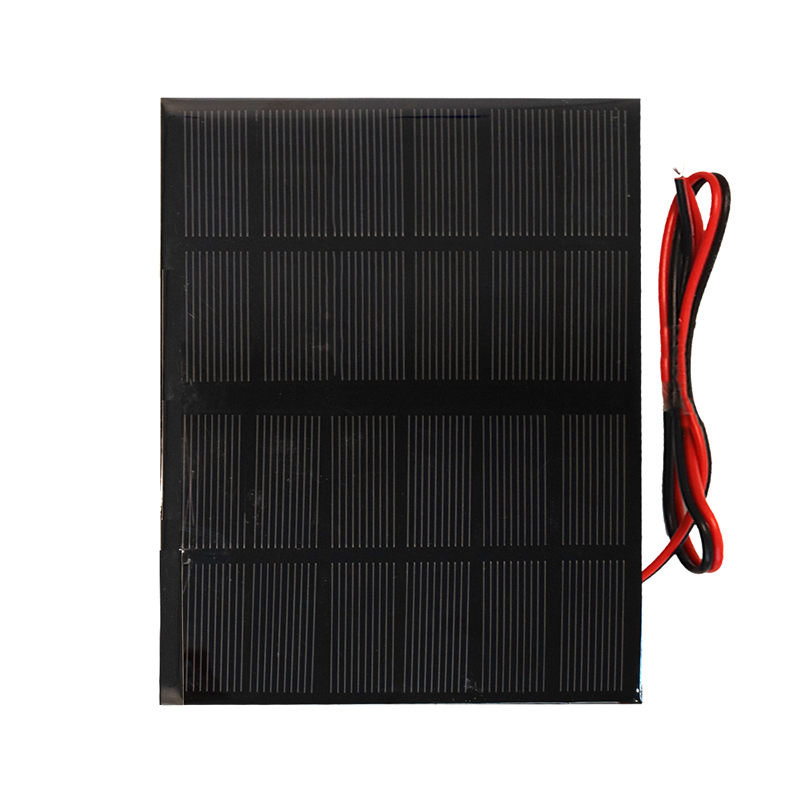
\includegraphics[scale = 0.1]{Documento/Imagenes/Análisis/Bat-Pan/Panel-Solar-6V.jpg}}
& \shortstack{\\ 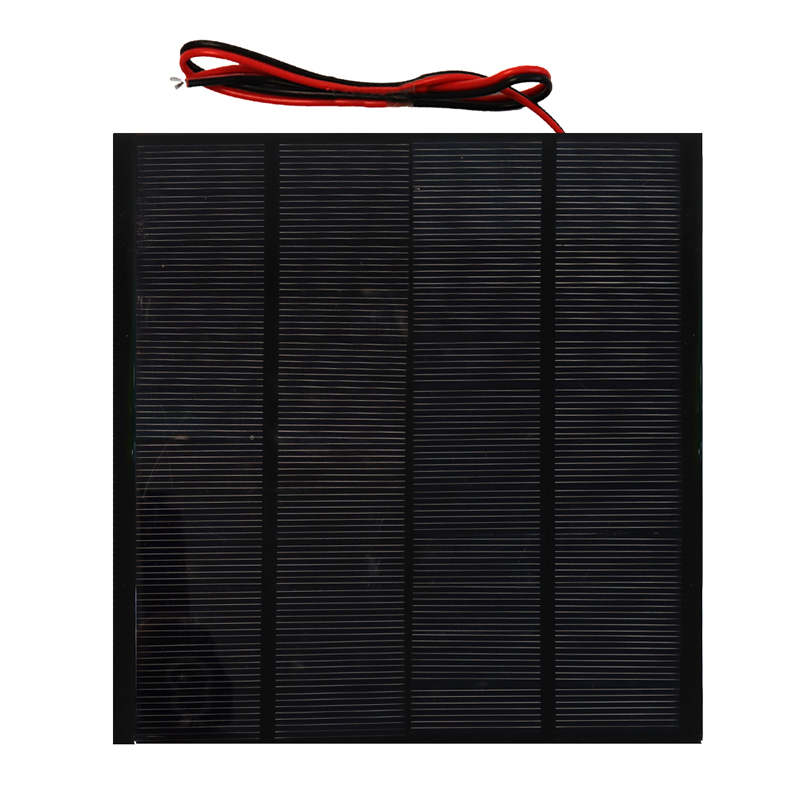
\includegraphics[scale = 0.1]{Documento/Imagenes/Análisis/Bat-Pan/Panel-Solar-12V.jpg}} \\
\hline
\end{tabular}
\end{table}

Se selecciona el \textbf{Panel Solar de \SI{6}{\volt} / \SI{1.92}{\watt}}. Aunque el panel de \SI{5}{\volt} ofrece características similares, el voltaje ligeramente superior del panel de \SI{6}{\volt} proporciona un mayor margen para la caída de tensión y es óptimo para módulos de carga como el CN3065, que requieren un voltaje de entrada superior al de la batería \cite{chipCN3065}. Además, este modelo es el más compacto y económico de las opciones evaluadas \cite{panelSolar6V}. El panel de \SI{12}{\volt} está sobredimensionado y es menos eficiente para cargar una batería de \SI{3.7}{\volt} con un cargador simple.

\paragraph{Análisis de Generación vs. Consumo:}
\begin{itemize}
    \item Consumo Diario Promedio: $\SI{47.6}{\milli\ampere\hour / \text{semana}} / 7\,\text{días} \approx \SI{6.8}{\milli\ampere\hour / \text{día}}$.
    \item Generación Diaria Estimada: Asumiendo un promedio conservador de \textbf{3 horas} de sol directo equivalente por día (HSP - Horas Solares Pico) para la Ciudad de México \cite{solarGIS}, la energía generada es:
    \begin{equation} \label{eq:generacion_diaria}
    \text{Generación}_{\text{diaria}} = I_{\text{mp}} \times \text{HSP} = \SI{320}{\milli\ampere} \times \SI{3}{\hour} = \SI{960}{\milli\ampere\hour}
    \end{equation}
\end{itemize}
El excedente energético diario ($\text{Generación}_{\text{diaria}} - \text{Consumo}_{\text{diario}} \approx \SI{953}{\milli\ampere\hour}$) es extremadamente amplio (más de 140 veces el consumo diario), lo que garantiza la recarga completa de la batería incluso bajo condiciones de irradiación solar subóptimas (días nublados, sombra parcial). El tiempo teórico necesario para reponer el consumo de una semana completa con sol directo sería mínimo: $\SI{47.6}{\milli\ampere\hour} / \SI{320}{\milli\ampere} \approx \SI{0.15}{\hour} \approx \SI{9}{\minute}$.

\subsection{Análisis de módulos de carga}

El módulo de carga es el componente encargado de gestionar la recarga segura de la batería desde el panel solar. Su función principal es proteger la batería contra sobrecargas, sobredescargas y controlar el flujo de corriente, lo cual es esencial para extender su vida útil. Esta subsección presenta una comparativa entre distintos módulos de carga compatibles con baterías Li-ion o LiPo, considerando su capacidad de carga, compatibilidad con paneles solares, protección integrada y facilidad de integración con el sistema(Tabla \ref{tab:modulos_carga}).

\renewcommand{\arraystretch}{1.5}
\begin{longtable}{|p{4.5cm}|c|c|c|}
\caption{Comparativa de módulos de carga para baterías recargables}
\label{tab:modulos_carga} \\
\hline
\textbf{Característica} & \textbf{CN3065} \cite{chipCN3065}
                        & \textbf{SD05CRMA} \cite{SD05CRMA}
                        & \textbf{CN3791} \cite{chipCN3791} \\
\hline
\endfirsthead

\hline
\textbf{Característica} & \textbf{CN3065} \cite{chipCN3065}
                        & \textbf{SD05CRMA} \cite{SD05CRMA}
                        & \textbf{CN3791} \cite{chipCN3791} \\
\hline
\endhead

\hline
\multicolumn{4}{r}{\textit{Continúa en la siguiente página}} \\
\endfoot

\hline
\endlastfoot

Tipo de batería compatible & Li-ion/Li-Po & Li-ion/Li-Po & Li-ion \\
\hline
Voltaje de entrada (V) & 4.4 - 6 & 4.4 - 6 & 4.5 - 28 \\
\hline
Corriente máxima de carga (mA) & 1000 & 1000 & 4000 \\
\hline
Protección integrada (sobre/descarga) & Sí & Sí & Sí \\
\hline
Compatibilidad con panel solar & Sí & Sí & Sí \\
\hline
Tamaño (mm) & 40x20x7 & 10.3x18.3 & 45x20 \\
\hline
Precio aproximado (USD) & \$2 & \$3 & \$4 \\
\hline
Imagen 
& 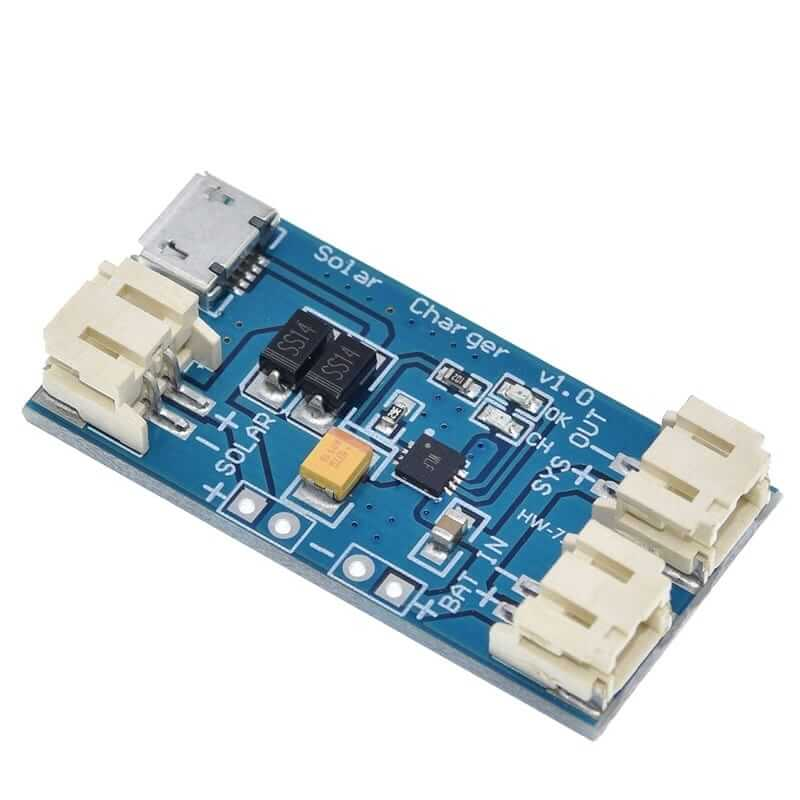
\includegraphics[scale=0.1]{Documento/Imagenes/Análisis/Bat-Pan/Cargador-Solar.jpg}
& 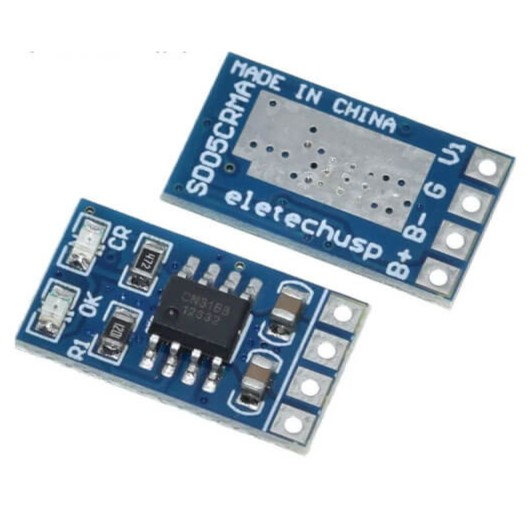
\includegraphics[scale=0.17]{Documento/Imagenes/Análisis/Bat-Pan/Cargador-SD05CRMA.jpg}
& 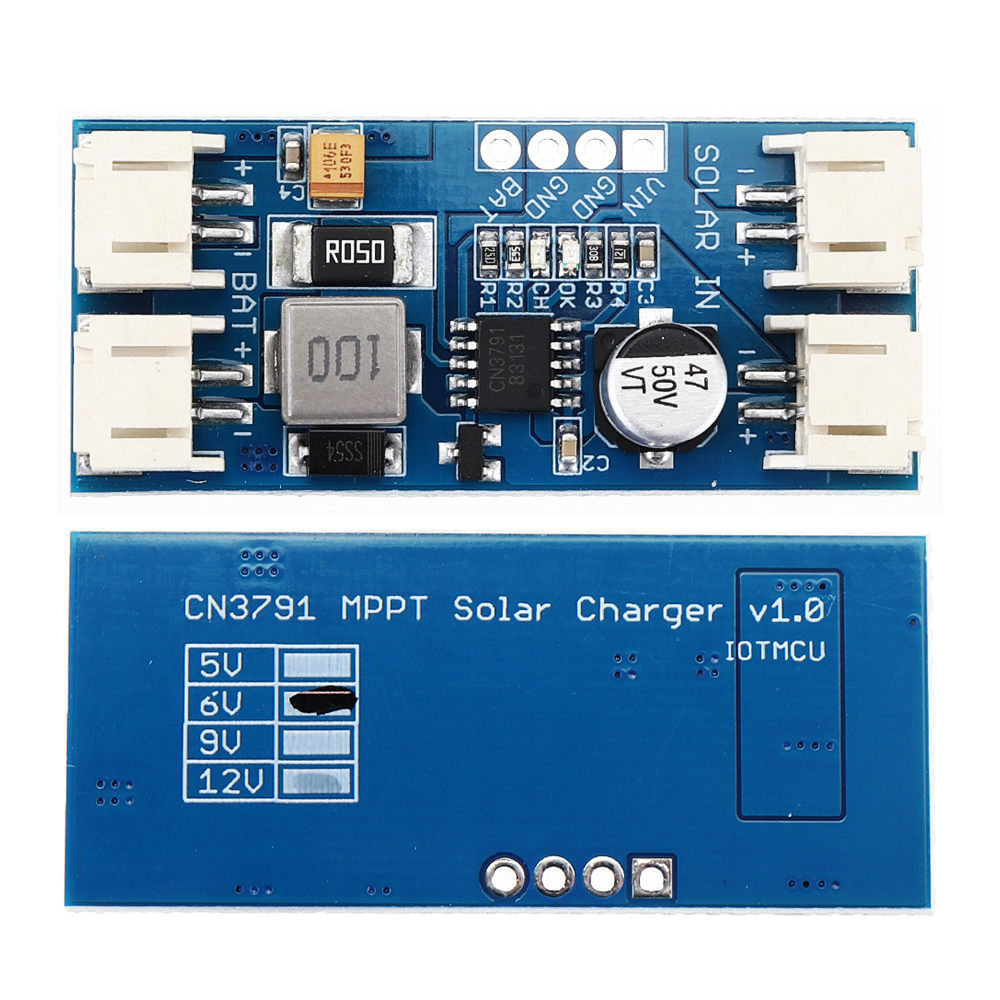
\includegraphics[scale=0.1]{Documento/Imagenes/Análisis/Bat-Pan/Cargador-CN3791.jpg} \\
\end{longtable}

Se selecciona el módulo basado en el chip \textbf{CN3065}. Este circuito integrado está específicamente diseñado para la carga de baterías de litio de una celda directamente desde paneles solares de bajo voltaje (\SIrange{4.4}{6}{\volt}), coincidiendo perfectamente con el panel seleccionado \cite{chipCN3065}. Incluye las protecciones esenciales (sobrecarga, sobredescarga a través de pines dedicados si se usa un IC externo) y regula la corriente de carga (hasta \SI{500}{\milli\ampere}), lo cual es adecuado para la corriente generada por el panel (\SI{320}{\milli\ampere}).

Los módulos basados en el popular chip TP4056, aunque económicos, están optimizados para carga a través de USB (\SI{5}{\volt}) y no manejan de forma nativa la variabilidad de voltaje de un panel solar \cite{chipTP4056}. El módulo CN3791, si bien incluye MPPT (Maximum Power Point Tracking) para maximizar la extracción de energía del panel, representa una complejidad y costo innecesarios dado el enorme excedente energético ya calculado; el MPPT es más beneficioso en sistemas con paneles más grandes o consumos mucho más ajustados \cite{chipCN3791}. Por lo tanto, el CN3065 ofrece la solución más simple, económica y adecuada para este sistema.


%%%%%%%%%%%%%%%%%%%%%%%%%%%%%%%%%%%%%%%%%%%%%%%%%%%%
%             SECCIÓN: Cálculo de residuos         %
%%%%%%%%%%%%%%%%%%%%%%%%%%%%%%%%%%%%%%%%%%%%%%%%%%%%

\section{Análisis de la medición de residuos sólidos flotantes en cuerpos de agua lóticos}

La acumulación de residuos sólidos flotantes representa un problema creciente en cuerpos de agua lóticos como ríos y arroyos, debido a su capacidad para transportar contaminantes desde zonas urbanas, agrícolas o industriales hacia cuerpos receptores mayores. Estos residuos, compuestos principalmente por plásticos, envases, metales y material no biodegradable, afectan no solo la estética del entorno natural, sino también la salud ambiental y humana.

Según las guías operacionales de la UNEP/IOC, las evaluaciones de basura flotante en ambientes marinos deben considerar tanto la recolección mediante redes superficiales ("trawl surveys") como observaciones visuales sistemáticas desde plataformas móviles \cite{cheshire2009directrices}. Al adaptar estas estrategias a cuerpos de agua interiores, se propone una metodología de monitoreo basada en:

\begin{itemize}
    \item \textbf{Captura de imágenes periódicas:} mediante cámaras fijas instaladas en puntos estratégicos del río. Estas imágenes permitirán realizar una estimación visual de la cantidad de residuos sólidos flotantes.
    \item \textbf{Frecuencia de muestreo adaptada:} al comportamiento hidrodinámico del cuerpo de agua y a los patrones locales de generación de basura. Por ejemplo, se sugiere capturar imágenes diariamente o durante eventos climáticos relevantes (lluvias, crecidas).
    \item \textbf{Plataforma de análisis automatizado:} que en fases posteriores permitirá integrar algoritmos de visión por computadora para la clasificación y cuantificación automática de los residuos identificados.
\end{itemize}

La implementación de este módulo de monitoreo visual no busca sustituir técnicas de muestreo físico, sino complementarlas al proporcionar una evaluación continua y no invasiva de la contaminación superficial. Esta información puede utilizarse para calcular indicadores como densidad de residuos (elementos por metro cuadrado de superficie visible) o tasa de acumulación, adaptando los métodos sugeridos por la \textit{UNEP/IOC} al contexto fluvial.

\subsection{Cálculo de densidad temporal de residuos flotantes}

Para cuantificar la cantidad de residuos sólidos flotantes observados en un tramo de río durante un intervalo de tiempo determinado, se utiliza la siguiente expresión para calcular la densidad temporal:

\begin{equation}
D_t = \frac{N_t}{A \cdot \Delta t}
\label{eq:densidad_basura_tiempo}
\end{equation}

Donde:
\begin{itemize}
    \item $D_t$ es la densidad temporal de residuos (elementos/m²/unidad de tiempo),
    \item $N_t$ es el número total de residuos observados durante el intervalo $\Delta t$,
    \item $A$ es el área superficial observada (en metros cuadrados),
    \item $\Delta t$ es el intervalo de tiempo de observación (en horas, días, etc.).
\end{itemize}

Esta fórmula permite calcular la tasa de acumulación de residuos flotantes en la superficie del agua, lo cual es útil para identificar zonas críticas de contaminación o evaluar el impacto de eventos específicos (como lluvias o descargas urbanas) sobre el ingreso de residuos. Esta función será realizada por los nodos con cámara OV2640/OV5640 integrados en la red inalámbrica, que operan de forma autónoma y sincronizada con el resto del sistema de monitoreo. La estimación visual depende de variables como el campo de visión efectivo de la cámara, la reflectancia de los residuos, la turbidez del agua y las condiciones de luz ambiental. Estos factores pueden introducir incertidumbre en los parámetros $N_t$ y $A$ de la ecuación.



%%%%%%%%%%%%%%%%%%%%%%%%%%%%%%%%%%%%%%%%%%%%%%%%%%%%
%             SECCIÓN: Servidores                  %
%%%%%%%%%%%%%%%%%%%%%%%%%%%%%%%%%%%%%%%%%%%%%%%%%%%%

\section{Análisis de Servidor}

El servidor constituye el núcleo central de la arquitectura del sistema, operando bajo el modelo cliente-servidor, donde actúa como proveedor de recursos y servicios para los nodos de la red y la interfaz web \cite{supermicro2024}. La selección de una plataforma de servidor adecuada es crítica para garantizar la escalabilidad, fiabilidad y rendimiento del sistema, especialmente considerando el procesamiento de imágenes y la gestión de series temporales de datos.

El análisis se centra en dos modelos de despliegue principales: servidores locales (\textit{on-premise}) y servidores en la nube (\textit{cloud computing}), evaluando su idoneidad frente a los requerimientos del proyecto.

\subsection{Requerimientos Clave del Servidor}
\label{subsec:reqs_servidor}

Para cumplir con sus funciones, la plataforma servidora debe satisfacer los siguientes requerimientos técnicos:

\begin{enumerate}
    \item \textbf{Capacidad de Cómputo:} Debe disponer de recursos de CPU (y opcionalmente GPU) suficientes para ejecutar el algoritmo de visión artificial (YOLO) para la detección de residuos en las imágenes recibidas.
    \item \textbf{Almacenamiento Escalable:} Requiere una solución de almacenamiento capaz de gestionar eficientemente tanto los datos estructurados de los sensores (series temporales) como los datos no estructurados (imágenes en formato JPEG).
    \item \textbf{Alta Disponibilidad y Fiabilidad:} El sistema debe operar de forma continua para recibir y procesar los datos de la WSN sin interrupciones.
    \item \textbf{Conectividad de Red:} Debe contar con una conexión a internet estable y de ancho de banda suficiente para recibir los datos del nodo concentrador y servir la interfaz web.
    \item \textbf{Seguridad:} Es imperativo implementar medidas de seguridad para proteger la integridad y confidencialidad de los datos, así como para controlar el acceso a la API.
    \item \textbf{Viabilidad Económica:} La solución debe ser rentable, considerando los costos iniciales y operativos a largo plazo.
\end{enumerate}

\subsection{Comparativa de Modelos de Despliegue}
\label{subsec:modelos_despliegue}

Se evaluaron dos paradigmas fundamentales para la implementación del servidor:

\begin{itemize}
    \item \textbf{Servidor Local (On-Premise):} Implica la adquisición y mantenimiento de hardware físico en una ubicación controlada. El equipo es responsable de la instalación, configuración y seguridad \cite{nordlayer2024}.
        \begin{itemize}
            \item \textit{Ventajas:} Control total sobre el hardware y los datos, lo cual puede ser preferible para cumplir con estrictas normativas de cumplimiento regulatorio \cite{nordlayer2024}.
            \item \textit{Desventajas:} Alta inversión inicial en hardware y licencias, complejidad en la gestión, escalabilidad limitada y necesidad de asegurar la infraestructura de soporte (energía, red) \cite{softteco2024}.
        \end{itemize}
    \item \textbf{Servidor en la Nube (Cloud):} Utiliza un modelo para el acceso bajo demanda a un conjunto compartido de recursos de cómputo configurables que pueden ser rápidamente aprovisionados con un esfuerzo de gestión mínimo \cite{mell2011nist}.
        \begin{itemize}
            \item \textit{Ventajas:} Alta escalabilidad y elasticidad, fiabilidad garantizada por el proveedor (SLA), seguridad robusta y un modelo de costos basado en el pago por uso que elimina la inversión inicial en hardware \cite{softteco2024}.
            \item \textit{Desventajas:} Costos operativos recurrentes y dependencia de la conectividad a internet \cite{softteco2024}.
        \end{itemize}
\end{itemize}

\subsection{Análisis de Proveedores de Servicios en la Nube}
\label{subsec:proveedores_nube}

Dado que el proyecto requiere flexibilidad, escalabilidad y alta disponibilidad, el modelo de servidor en la nube se identifica como el más adecuado. A continuación, se comparan los tres principales proveedores de servicios en la nube, reconocidos como líderes en el sector por analistas de la industria como Gartner \cite{gartner2023magic}.

\renewcommand{\arraystretch}{1.5}
\begin{longtable}{
    |p{2.5cm}   % Columna 1: Característica
    |p{4.2cm}   % Columna 2: AWS
    |p{4.2cm}   % Columna 3: GCP
    |p{4.2cm}|  % Columna 4: Azure
}
\caption{Comparativa de Plataformas de Servidor en la Nube}
\label{tab:comparativa_cloud} \\
\hline
\textbf{Característica} 
    & \textbf{Amazon Web Services (AWS)} 
    & \textbf{Google Cloud Platform (GCP)} 
    & \textbf{Microsoft Azure} \\
\hline
\endfirsthead

\hline
\textbf{Característica} 
    & \textbf{Amazon Web Services (AWS)} 
    & \textbf{Google Cloud Platform (GCP)} 
    & \textbf{Microsoft Azure} \\
\hline
\endhead

\hline
\multicolumn{4}{r}{\textit{Continúa en la siguiente página}} \\
\endfoot

\hline
\endlastfoot

Cómputo 
    & \textbf{EC2} (Elastic Compute Cloud). Máquinas virtuales escalables con una amplia variedad de instancias, incluyendo las optimizadas para GPU \cite{qainsights2024}. 
    & \textbf{Compute Engine}. Máquinas virtuales de alto rendimiento. Fuerte enfoque en cargas de trabajo de IA y Machine Learning \cite{googlecloud2024products}. 
    & \textbf{Virtual Machines}. Servidores virtuales con una profunda integración con el ecosistema de Microsoft y Windows Server \cite{azure2024products}. \\ \hline

Almacenamiento 
    & \textbf{S3} (Simple Storage Service). Almacenamiento de objetos líder en la industria, diseñado para una durabilidad del 99.999999999\% \cite{qainsights2024}. 
    & \textbf{Cloud Storage}. Almacenamiento de objetos seguro y escalable, con diferentes clases de almacenamiento para optimizar costos \cite{googlecloud2024products}. 
    & \textbf{Blob Storage}. Solución de almacenamiento masivo para datos no estructurados como imágenes y videos \cite{azure2024storage}. \\ \hline

Base de Datos 
    & \textbf{RDS} (Relational Database Service) para SQL (ej. PostgreSQL) y \textbf{DynamoDB} para NoSQL de alto rendimiento \cite{qainsights2024}. 
    & \textbf{Cloud SQL} para bases de datos relacionales gestionadas y \textbf{Firestore/Bigtable} para soluciones NoSQL \cite{googlecloud2024sql}. 
    & \textbf{Azure SQL Database} para bases de datos SQL gestionadas y \textbf{Cosmos DB} para necesidades NoSQL multimodelo y distribuidas globalmente \cite{azure2024products}. \\ \hline

Servicios IoT 
    & \textbf{AWS IoT Core}. Plataforma completa para la conexión segura y gestión de millones de dispositivos, con enrutamiento de mensajes \cite{varonis2024}. 
    & \textbf{Cloud IoT Core}. Servicio gestionado para la ingesta segura de datos de dispositivos IoT (actualmente en transición a servicios de partners). 
    & \textbf{Azure IoT Hub}. Servicio escalable para la comunicación bidireccional fiable y segura entre la aplicación y los dispositivos \cite{varonis2024}. \\ \hline

Costo 
    & Modelo de pago por uso. Ofrece una capa gratuita (\textit{Free Tier}) por 12 meses, ideal para prototipos \cite{coursera2024}. 
    & Precios competitivos con descuentos por uso sostenido. Ofrece créditos iniciales y una capa gratuita competitiva \cite{datacamp2024}. 
    & Modelo de pago por uso con ventajas como el \textit{Hybrid Benefit} para clientes con licencias de Microsoft existentes \cite{varonis2024}. \\ \hline

\end{longtable}



Considerando los requerimientos del proyecto, se selecciona una arquitectura basada en la nube como la solución óptima. Entre los proveedores, \textbf{Amazon Web Services (AWS)} se elige como la plataforma para el desarrollo de este prototipo. La justificación se basa en los siguientes puntos:

\begin{enumerate}
    \item \textbf{Madurez y Ecosistema:} AWS es la plataforma más madura y con la mayor cuota de mercado, ofreciendo el ecosistema de servicios más amplio y una vasta documentación \cite{coursera2024}.
    \item \textbf{Capa Gratuita Robusta:} El \textit{Free Tier} de AWS permite desplegar los recursos necesarios para un prototipo funcional (ej. EC2, S3, RDS) sin costo durante el primer año, lo cual es ideal para un proyecto de tesis \cite{aws2024freetier}.
    \item \textbf{Servicios IoT Integrados:} AWS IoT Core proporciona una solución robusta y bien documentada para gestionar la comunicación desde el nodo concentrador, simplificando la autenticación de dispositivos y la ingesta de datos.
\end{enumerate}

La arquitectura de servicios propuesta en AWS consistiría en:
\begin{itemize}
    \item Un servidor de cómputo virtual (\textbf{Amazon EC2}) para ejecutar el \textit{backend} de la aplicación y el algoritmo de visión artificial.
    \item Un servicio de almacenamiento de objetos (\textbf{Amazon S3}) para el almacenamiento durable de las imágenes capturadas.
    \item Un \textbf{servicio de base de datos gestionada} para la persistencia, integridad y consulta de los datos de los sensores y los metadatos de las imágenes.
    \item Un servicio de conexión de dispositivos (\textbf{AWS IoT Core}) para gestionar la comunicación segura desde el nodo concentrador.
\end{itemize}

La selección específica del motor y el tipo de servicio de base de datos se justifica en detalle en la siguiente sección, basándose en un análisis de los modelos de datos del proyecto.


%%%%%%%%%%%%%%%%%%%%%%%%%%%%%%%%%%%%%%%%%%%%%%%%%%%%
%             SECCIÓN: Bases de datos              %
%%%%%%%%%%%%%%%%%%%%%%%%%%%%%%%%%%%%%%%%%%%%%%%%%%%%

\section{Análisis de Base de Datos}
\label{sec:analisis_db}

La base de datos es un componente crítico del servidor, responsable de la persistencia, integridad y disponibilidad de los datos generados por la WSN. La elección de una tecnología de base de datos adecuada impacta directamente en el rendimiento de las consultas, la escalabilidad del sistema y la facilidad con la que se pueden realizar análisis históricos.

\subsection{Requerimientos de la Base de Datos}
\label{subsec:reqs_db}

Con base en la arquitectura del sistema, la base de datos debe cumplir con los siguientes requerimientos específicos:

\begin{enumerate}
    \item \textbf{Manejo de Series Temporales:} El sistema debe almacenar eficientemente las mediciones de los sensores (pH, turbidez, etc.), que son datos de series temporales, caracterizados por tener una marca de tiempo (\textit{timestamp}) y un valor \cite{influxdata2024timeseries}. Esto requiere optimización para inserciones rápidas y consultas complejas basadas en rangos de tiempo.
    \item \textbf{Almacenamiento de Metadatos de Imágenes:} Debe gestionar los metadatos asociados a cada imagen capturada, incluyendo la URL de almacenamiento, la marca de tiempo, la identificación del nodo sensor y los resultados del análisis de visión artificial.
    \item \textbf{Escalabilidad:} La base de datos debe ser capaz de escalar horizontalmente para manejar el volumen creciente de datos a medida que la red de sensores opera a lo largo del tiempo o se expande con nuevos nodos \cite{mongodb2024scalability}.
    \item \textbf{Integridad y Consistencia:} Debe garantizar la integridad de los datos, asegurando que las mediciones se almacenen de forma fiable y consistente, siguiendo principios como los definidos por el modelo ACID en sistemas transaccionales \cite{oracle2024acid}.
    \item \textbf{Rendimiento de Consultas:} El sistema debe permitir consultas de baja latencia para alimentar la interfaz web con datos históricos y en tiempo real.
\end{enumerate}

\subsection{Análisis de Modelos de Base de Datos: SQL vs. NoSQL}
%\label{subsec:modelos_db}

Para satisfacer estos requerimientos, se analizaron los dos modelos de bases de datos predominantes: relacional (SQL) y no relacional (NoSQL).

\begin{itemize}
    \item \textbf{Bases de Datos Relacionales (SQL):} Organizan los datos en tablas estructuradas con un esquema predefinido y son conocidas por su robustez y consistencia (propiedades ACID) \cite{oracle2024sql}. Son muy adecuadas para almacenar los metadatos de las imágenes y las relaciones entre nodos y mediciones \cite{mongodb2024sqlvsnosql}.
    \item \textbf{Bases de Datos No Relacionales (NoSQL):} Utilizan modelos de datos flexibles y priorizan la escalabilidad y la disponibilidad, a menudo siguiendo el modelo BASE (Basically Available, Soft state, Eventually consistent) \cite{mongodb2024sqlvsnosql}. Son ideales para el almacenamiento de datos de series temporales, donde el volumen de inserciones es alto \cite{aws2024sqlvsnosql}.
\end{itemize}

\subsection{Comparativa de Servicios de Base de Datos en AWS}
\label{subsec:comparativa_db_aws}

Dada la selección de AWS como proveedor de nube, se comparan sus servicios de bases de datos gestionadas más relevantes, incluyendo opciones relacionales y una opción especializada en series temporales.

\begin{table}[H]
\centering
\caption{Comparativa de Servicios de Base de Datos Gestionadas en AWS}
\label{tab:comparativa_db}
\resizebox{\textwidth}{!}{%
\begin{tabular}{|l|p{3.2cm}|p{3.2cm}|p{3.2cm}|p{3.2cm}|}
\hline
\textbf{Característica} & \textbf{Amazon RDS para PostgreSQL} & \textbf{Amazon RDS para MySQL} & \textbf{Amazon Aurora} & \textbf{Amazon Timestream} \\
\hline
\textbf{Modelo} & Relacional (SQL) & Relacional (SQL) & Relacional (SQL), compatible con PostgreSQL y MySQL & NoSQL (Series Temporales) \\
\hline
\textbf{Caso de Uso Principal} & Aplicaciones que requieren consultas complejas, manejo de datos geoespaciales y extensibilidad \cite{aws2024rds}. & Aplicaciones web de propósito general, CMS y comercio electrónico. Muy popular en el ecosistema LAMP \cite{aws2024rds}. & Cargas de trabajo de alto rendimiento y alta disponibilidad a escala de nube. Aplicaciones empresariales críticas \cite{aws2024aurora}. & Monitoreo de IoT, análisis de datos de telemetría y series temporales a gran escala \cite{aws2024timestream}. \\
\hline
\textbf{Fortalezas Clave} & Soporte avanzado de tipos de datos y extensiones (ej. PostGIS). Cumplimiento estricto del estándar SQL. & Simplicidad, facilidad de uso y un ecosistema muy maduro. Buen rendimiento para lecturas. & Rendimiento hasta 3 veces superior a PostgreSQL estándar. Almacenamiento auto-reparable y distribuido. & Optimizado para ingesta masiva de datos temporales. Arquitectura de almacenamiento de dos niveles (memoria y magnético). \\
\hline
\textbf{Escalabilidad} & Escala verticalmente y horizontalmente mediante réplicas de lectura. & Escala verticalmente y horizontalmente mediante réplicas de lectura. & Escalabilidad superior con hasta 15 réplicas de lectura. Almacenamiento que escala automáticamente. & Escala horizontalmente de forma automática y sin servidor (\textit{serverless}). \\
\hline
\textbf{Costo} & Basado en horas de instancia y almacenamiento. Parte del \textit{Free Tier} \cite{aws2024rdsprice}. & Basado en horas de instancia y almacenamiento. Parte del \textit{Free Tier} \cite{aws2024rdsprice}. & Modelo de precios basado en el consumo, más costoso que RDS estándar. No forma parte del \textit{Free Tier} \cite{aws2024auroraprice}. & Basado en volumen de datos escritos, almacenados y consultados. Muy rentable para grandes volúmenes \cite{aws2024timestreamprice}. \\
\hline
\end{tabular}%
}
\end{table}

Tras analizar los requerimientos y las plataformas disponibles, se ha decidido optar por una \textbf{arquitectura de base de datos unificada} para simplificar el diseño del sistema, reducir la complejidad operativa y centralizar la gestión de los datos.

La elección se inclina hacia un sistema de gestión de bases de datos relacional (RDBMS), ya que ofrece la versatilidad necesaria para manejar tanto los datos estructurados de los metadatos como las series temporales de los sensores, garantizando al mismo tiempo la máxima integridad de los datos.

Entre las opciones relacionales evaluadas, se selecciona \textbf{Amazon RDS para PostgreSQL} como la plataforma de base de datos única para el proyecto. Esta decisión se fundamenta en los siguientes puntos clave:

\begin{enumerate}
    \item \textbf{Versatilidad y Potencia:} PostgreSQL es conocido por su robustez y su estricto cumplimiento del estándar SQL. Es capaz de gestionar eficientemente los datos relacionales (configuración de nodos, metadatos de imágenes) y, al mismo tiempo, puede ser optimizado para manejar cargas de trabajo de series temporales mediante técnicas avanzadas como la partición de tablas por rangos de fecha y el uso de índices especializados, asegurando un buen rendimiento en las consultas temporales.
    
    \item \textbf{Superioridad para Datos Complejos:} En comparación con MySQL, PostgreSQL ofrece un manejo más avanzado de tipos de datos complejos y un ecosistema de extensiones más rico, como \textbf{PostGIS}, que podría ser crucial en futuras fases del proyecto para realizar análisis geoespaciales sobre la ubicación de los nodos \cite{postgresql2024about}. Esta capacidad de extensión lo convierte en una opción más sólida y preparada para el futuro en aplicaciones científicas y de monitoreo.

    \item \textbf{Viabilidad para el Prototipo:} Amazon Aurora, aunque técnicamente superior en rendimiento, se descarta para esta fase debido a su mayor costo y a que sus capacidades exceden los requerimientos del prototipo. Por su parte, Amazon Timestream se descarta como solución única, ya que su modelo NoSQL no es el adecuado para gestionar las relaciones y la integridad de los metadatos del sistema.
\end{enumerate}

Por lo tanto, Amazon RDS para PostgreSQL representa el balance óptimo entre rendimiento, costo, integridad de los datos y flexibilidad, proporcionando una base sólida y unificada para todas las necesidades de almacenamiento del proyecto.


%%%%%%%%%%%%%%%%%%%%%%%%%%%%%%%%%%%%%%%%%%%%%%%%%%%%
%       SECCIÓN: Arquitectura de Cómputo           %
%%%%%%%%%%%%%%%%%%%%%%%%%%%%%%%%%%%%%%%%%%%%%%%%%%%%

\section{Análisis de Arquitectura de Cómputo para Visión Artificial}
\label{sec:analisis_edge_vs_cloud}

Una decisión de diseño fundamental en cualquier sistema de IoT que integra IA es determinar \textit{dónde} se realizará el procesamiento de los datos. Para la tarea de visión artificial de este proyecto, existen dos paradigmas principales: el cómputo en la nube y el cómputo en el borde \cite{shi2016edge}. A continuación, se analizan ambos enfoques.

\begin{itemize}
    \item \textbf{Cómputo en la Nube (\textit{Cloud Computing}):} En esta arquitectura, el dispositivo en el campo (el nodo sensor) actúa como un simple capturador de datos. Captura la imagen en bruto y la transmite a través de la red a un servidor centralizado y potente en la nube (ej. AWS EC2). Todo el procesamiento intensivo, como la ejecución del modelo YOLO, se realiza en el servidor.
        \begin{itemize}
            \item \textbf{Ventajas:} Permite el uso de modelos de IA muy grandes y precisos, ya que no hay restricciones de hardware. El nodo sensor puede ser más simple, económico y de menor consumo (excepto en la transmisión). La actualización y el mantenimiento del modelo de IA se centralizan en un solo lugar.
            \item \textbf{Desventajas:} Requiere un ancho de banda de red significativo y confiable para transmitir datos pesados (imágenes). La transmisión de grandes volúmenes de datos consume una cantidad considerable de energía, impactando la autonomía de la batería del nodo \cite{li2018learning}.
        \end{itemize}

    \item \textbf{Cómputo en el Borde (\textit{Edge Computing}):} En este enfoque, el procesamiento de los datos se realiza localmente, en o cerca del dispositivo que los captura. El nodo sensor estaría equipado con un microprocesador o microcontrolador más potente (ej. un acelerador de IA como un Coral Edge TPU) capaz de ejecutar una versión optimizada y ligera del modelo YOLO (\textit{e.g.}, YOLOv5n o un modelo cuantizado) \cite{chen2019deep}.
        \begin{itemize}
            \item \textbf{Ventajas:} Reduce drásticamente el tráfico de red. En lugar de enviar una imagen de 150 KB, el nodo solo transmite el resultado del análisis (unos pocos bytes de texto, ej. `{``objeto'': ``botella'', ``confianza'': 0.92}'). Esto se traduce en un ahorro masivo de energía en la comunicación inalámbrica y una mayor vida útil de la batería. También reduce la latencia y permite que el sistema funcione de forma autónoma si se pierde la conexión con el servidor central.
            \item \textbf{Desventajas:} Requiere hardware más potente y costoso en el nodo sensor. Limita el tamaño y la complejidad del modelo de IA que se puede ejecutar, lo que podría reducir la precisión en comparación con un modelo en la nube.
        \end{itemize}
\end{itemize}

Para la presente fase del proyecto, \textbf{se ha seleccionado la arquitectura de cómputo en la nube}. La justificación se basa en los siguientes criterios:

\begin{enumerate}
    \item \textbf{Flexibilidad y Precisión del Modelo:} El enfoque en la nube permite experimentar con diferentes versiones del modelo YOLO sin estar limitados por el hardware del nodo, priorizando la máxima precisión en la detección de residuos.
    \item \textbf{Simplicidad del Nodo Sensor:} Mantiene el diseño del hardware del nodo más simple y enfocado en la eficiencia energética para la captura y comunicación, lo cual es un desafío de por sí.
    \item \textbf{Viabilidad del Protocolo de Comunicación:} La elección del protocolo Wi-Fi HaLow, con su ancho de banda relativamente alto (comparado con LPWAN como LoRa), hace que la transmisión de imágenes comprimidas sea técnicamente viable, aunque energéticamente costosa.
\end{enumerate}

No obstante, se reconoce que una arquitectura de cómputo en el borde es una optimización altamente deseable. En el capítulo de ``Conclusiones y Trabajo Futuro", se propondrá la exploración de un modelo híbrido o de borde como una evolución natural de este sistema.




\section{Análisis de Modelos para Detección y Segmentación de Objetos}
\label{sec:analisis_vision}

La selección de un algoritmo adecuado para identificar y cuantificar los residuos sólidos flotantes es un componente central de la funcionalidad de visión artificial del sistema. Dada la necesidad de estimar la densidad de basura (posiblemente a través del área cubierta en píxeles), se requiere un modelo capaz no solo de detectar objetos (\textit{object detection}) sino también de delinear sus contornos precisos (\textit{instance segmentation}). La familia de modelos \textbf{YOLO (\textit{You Only Look Once})} ofrece arquitecturas que cubren ambas tareas con un buen balance entre velocidad y precisión \cite{sapkota2025yolo}. Se realizó un análisis comparativo para identificar la versión más apropiada.

\subsection{Criterios de Selección}
\label{subsec:criterios_vision}

La elección del modelo se basa en los siguientes criterios prioritarios:

\begin{enumerate}
    \item \textbf{Precisión (mAP / Mask mAP):} El modelo debe ofrecer alta precisión tanto en la detección (localización con cuadros delimitadores) como, preferiblemente, en la segmentación (delimitación a nivel de píxel). Se toma como referencia el rendimiento en el dataset COCO.
    \item \textbf{Capacidad de Segmentación Integrada:} Se valora positivamente que el modelo soporte la segmentación de instancias de forma nativa dentro de su framework, simplificando el entrenamiento y la inferencia.
    \item \textbf{Tamaño del Modelo y Requerimientos de Hardware:} Aunque el procesamiento se realizará en la nube, se prefiere un modelo con un tamaño razonable para facilitar su despliegue y gestión.
    \item \textbf{Facilidad de Uso y Ecosistema:} Disponibilidad de implementaciones robustas, buena documentación y una comunidad activa.
    \item \textbf{Flexibilidad para Re-entrenamiento:} Capacidad del modelo para ser afinado (\textit{fine-tuning}) con un dataset específico de residuos flotantes.
\end{enumerate}

\subsection{Comparativa de Modelos YOLO Relevantes}
\label{subsec:comparativa_yolo}

La Tabla \ref{tab:comparativa_yolo_condensada} presenta una comparativa de las versiones de YOLO consideradas, destacando su capacidad para la segmentación. Los valores de mAP corresponden al dataset COCO y dependen del hardware \cite{terven2023yolo, sapkota2025yolo}.

\renewcommand{\arraystretch}{1.3}
\begin{longtable}{
    |p{1.6cm}  % Modelo
    |p{1.7cm}         % Precisión
    |p{2.4cm}         % Segmentación
    |p{2.9cm}  % Requerimientos
    |p{2.1cm}         % Facilidad de uso
    |p{3.5cm}| % Ideal para
}
\caption{Comparativa de Modelos YOLO Relevantes (Dataset COCO)} \label{tab:comparativa_yolo_condensada} \\
\hline
\textbf{Modelo} & 
\textbf{Precisión (mAP Det.)} & 
\textbf{Soporte Segmentación Nativo?} & 
\textbf{Requerimientos Hardware (GPU)} & 
\textbf{Facilidad de Uso} & 
\textbf{Ideal Para} \\ 
\hline
\endfirsthead

\hline
\textbf{Modelo} & 
\textbf{Precisión (mAP Det.)} & 
\textbf{Soporte Segmentación Nativo?} & 
\textbf{Requerimientos Hardware (GPU)} & 
\textbf{Facilidad de Uso} & 
\textbf{Ideal Para} \\ 
\hline
\endhead

\hline
\multicolumn{6}{r}{\textit{Continúa en la siguiente página}} \\
\endfoot

\hline
\endlastfoot

YOLOv5 
& $\sim$ 55.8\% (v5x)
& No (Requiere forks/mods)
& Baja/Moderada (Básica a Media)
& Muy Alta (PyTorch Nativo)
& Detección rápida, buen balance, hardware moderado \\ \hline

YOLOv7 
& $\sim$ 56.8\% (v7x)
& No (Principalmente detección)
& Alta (Gama Alta)
& Moderada
& Detección de alta precisión y velocidad \\ \hline

YOLOv8 
& $\sim$ 53.9\% (v8x)
& \textbf{Sí} (Framework Unificado)
& Alta (Gama Alta)
& Muy Alta (Framework Ultralytics)
& \textbf{Detección y Segmentación}, versatilidad, estado del arte \\ \hline

YOLOv11 
& $\sim$ 55.4\% (Est.)
& \textbf{Sí} (Framework Unificado)
& Alta (Gama Alta)
& Alta (Reciente)
& Detección/Segmentación, mejoras arquitectónicas recientes \\ \hline

\multicolumn{6}{p{16cm}}{\footnotesize \textit{Nota: Los tamaños de modelo varían según la versión específica (n, s, m, l, x). El mAP corresponde a COCO val2017 para detección. La facilidad de uso de YOLOv11 puede variar por ser más reciente.}} \\

\end{longtable}


\subsection{Justificación y Selección del Modelo}
\label{subsec:justificacion_yolo}

La necesidad explícita de realizar segmentación de instancias para estimar la densidad de residuos mediante el área cubierta en píxeles inclina la balanza hacia modelos que ofrezcan esta funcionalidad de manera integrada y eficiente.

\begin{itemize}
    \item \textbf{YOLOv5:} Aunque es un modelo excelente y fácil de usar para la detección de objetos \cite{jocher2020yolov5}, no incluye la segmentación de instancias en su rama principal. Lograr segmentación requiere utilizar variantes o modificaciones específicas, lo que añade complejidad al desarrollo y mantenimiento.

    \item \textbf{YOLOv7:} Similar a YOLOv5, su enfoque principal ha sido optimizar la detección en términos de velocidad y precisión, sin integrar la segmentación como una tarea central.

    \item \textbf{YOLOv8:} Desarrollado por Ultralytics, se presenta como un framework unificado que maneja de forma nativa y eficiente tanto la detección como la segmentación de instancias, clasificación y estimación de pose \cite{ultralyticsYOLOv8}. Ofrece un rendimiento de vanguardia, es fácil de usar y cuenta con un excelente soporte y documentación.

    \item \textbf{YOLOv11:} Representa una de las evoluciones más recientes, prometiendo mejoras arquitectónicas \cite{sapkota2025yolo}. Aunque también soporta segmentación, al ser más nuevo, podría tener menos documentación comunitaria o requerir ajustes en las herramientas de entrenamiento en comparación con YOLOv8.
\end{itemize}

Considerando la necesidad de segmentación, la madurez relativa dentro de las arquitecturas modernas y la robustez del framework, se selecciona \textbf{YOLOv8-YOLOv11} como el modelo para este proyecto. Específicamente, se optará por una de sus variantes pre-entrenadas (ej. `yolov8s-seg.pt`) que ya incluye la capacidad de segmentación.

Esta elección ofrece el mejor compromiso entre:
\begin{itemize}
    \item \textbf{Funcionalidad Requerida:} Soporte nativo y eficiente para segmentación de instancias.
    \item \textbf{Precisión:} Rendimiento de vanguardia demostrado en benchmarks estándar.
    \item \textbf{Facilidad de Implementación:} Un framework unificado y bien documentado que simplifica el entrenamiento (fine-tuning) y la inferencia.
\end{itemize}

Si bien YOLOv5 sigue siendo una excelente opción si la detección simple fuese suficiente, la necesidad de cuantificar el área cubierta por los residuos hace que YOLOv8 sea la opción técnicamente superior para los objetivos planteados.





